\documentclass[a4paper,11pt,DIV=15,openany,twoside=false]{scrbook}

% everything inside \tthdump is ignored by tth, but processed by LaTeX
\newcommand{\tthdump}[1]{#1}

% include most packages
\tthdump{
  \usepackage[utf8]{inputenc}
  \usepackage[T1]{fontenc}
}
\usepackage{
  mathpazo,
  listings,
  braket,
  fancyvrb,
  booktabs,
  colortbl,
  mystuff,
  lastpage,
  array,
  longtable,
  framed,
  amsmath,
  amssymb,
  multirow,
  url,
  framed}
\usepackage[colorlinks=true,urlcolor=B,linkcolor=B,citecolor=R]{hyperref}
\usepackage[square, sort&compress, numbers]{natbib}
% hide some packages from tth
\tthdump{
  \usepackage[version=3]{mhchem}
  \usepackage{tikz,pgfplots}
  \pgfplotsset{compat=1.3}
}


% Bold caption labels
\tthdump{
  \setkomafont{captionlabel}{\bfseries}
}

% Paragraph settings
\setlength{\parindent}{0pt}
\setlength{\parskip}{\smallskipamount}
% use a different parsep for lists
\usepackage{enumitem}
\setlist[itemize]{parsep=0pt}
\setlist[enumerate]{parsep=0pt}

% no clubs and widows
\clubpenalty = 2000
\widowpenalty = 2000 
\displaywidowpenalty = 2000


% =============================== TITLE ==========================
%%tth: \title{SHARC: Surface Hopping in the Adiabatic Representation Including Arbitrary Couplings -- Manual}
\newenvironment{tpage}{%
\addtokomafont{title}{\rmfamily}
  \begin{titlepage}
    \title{\hspace{1cm}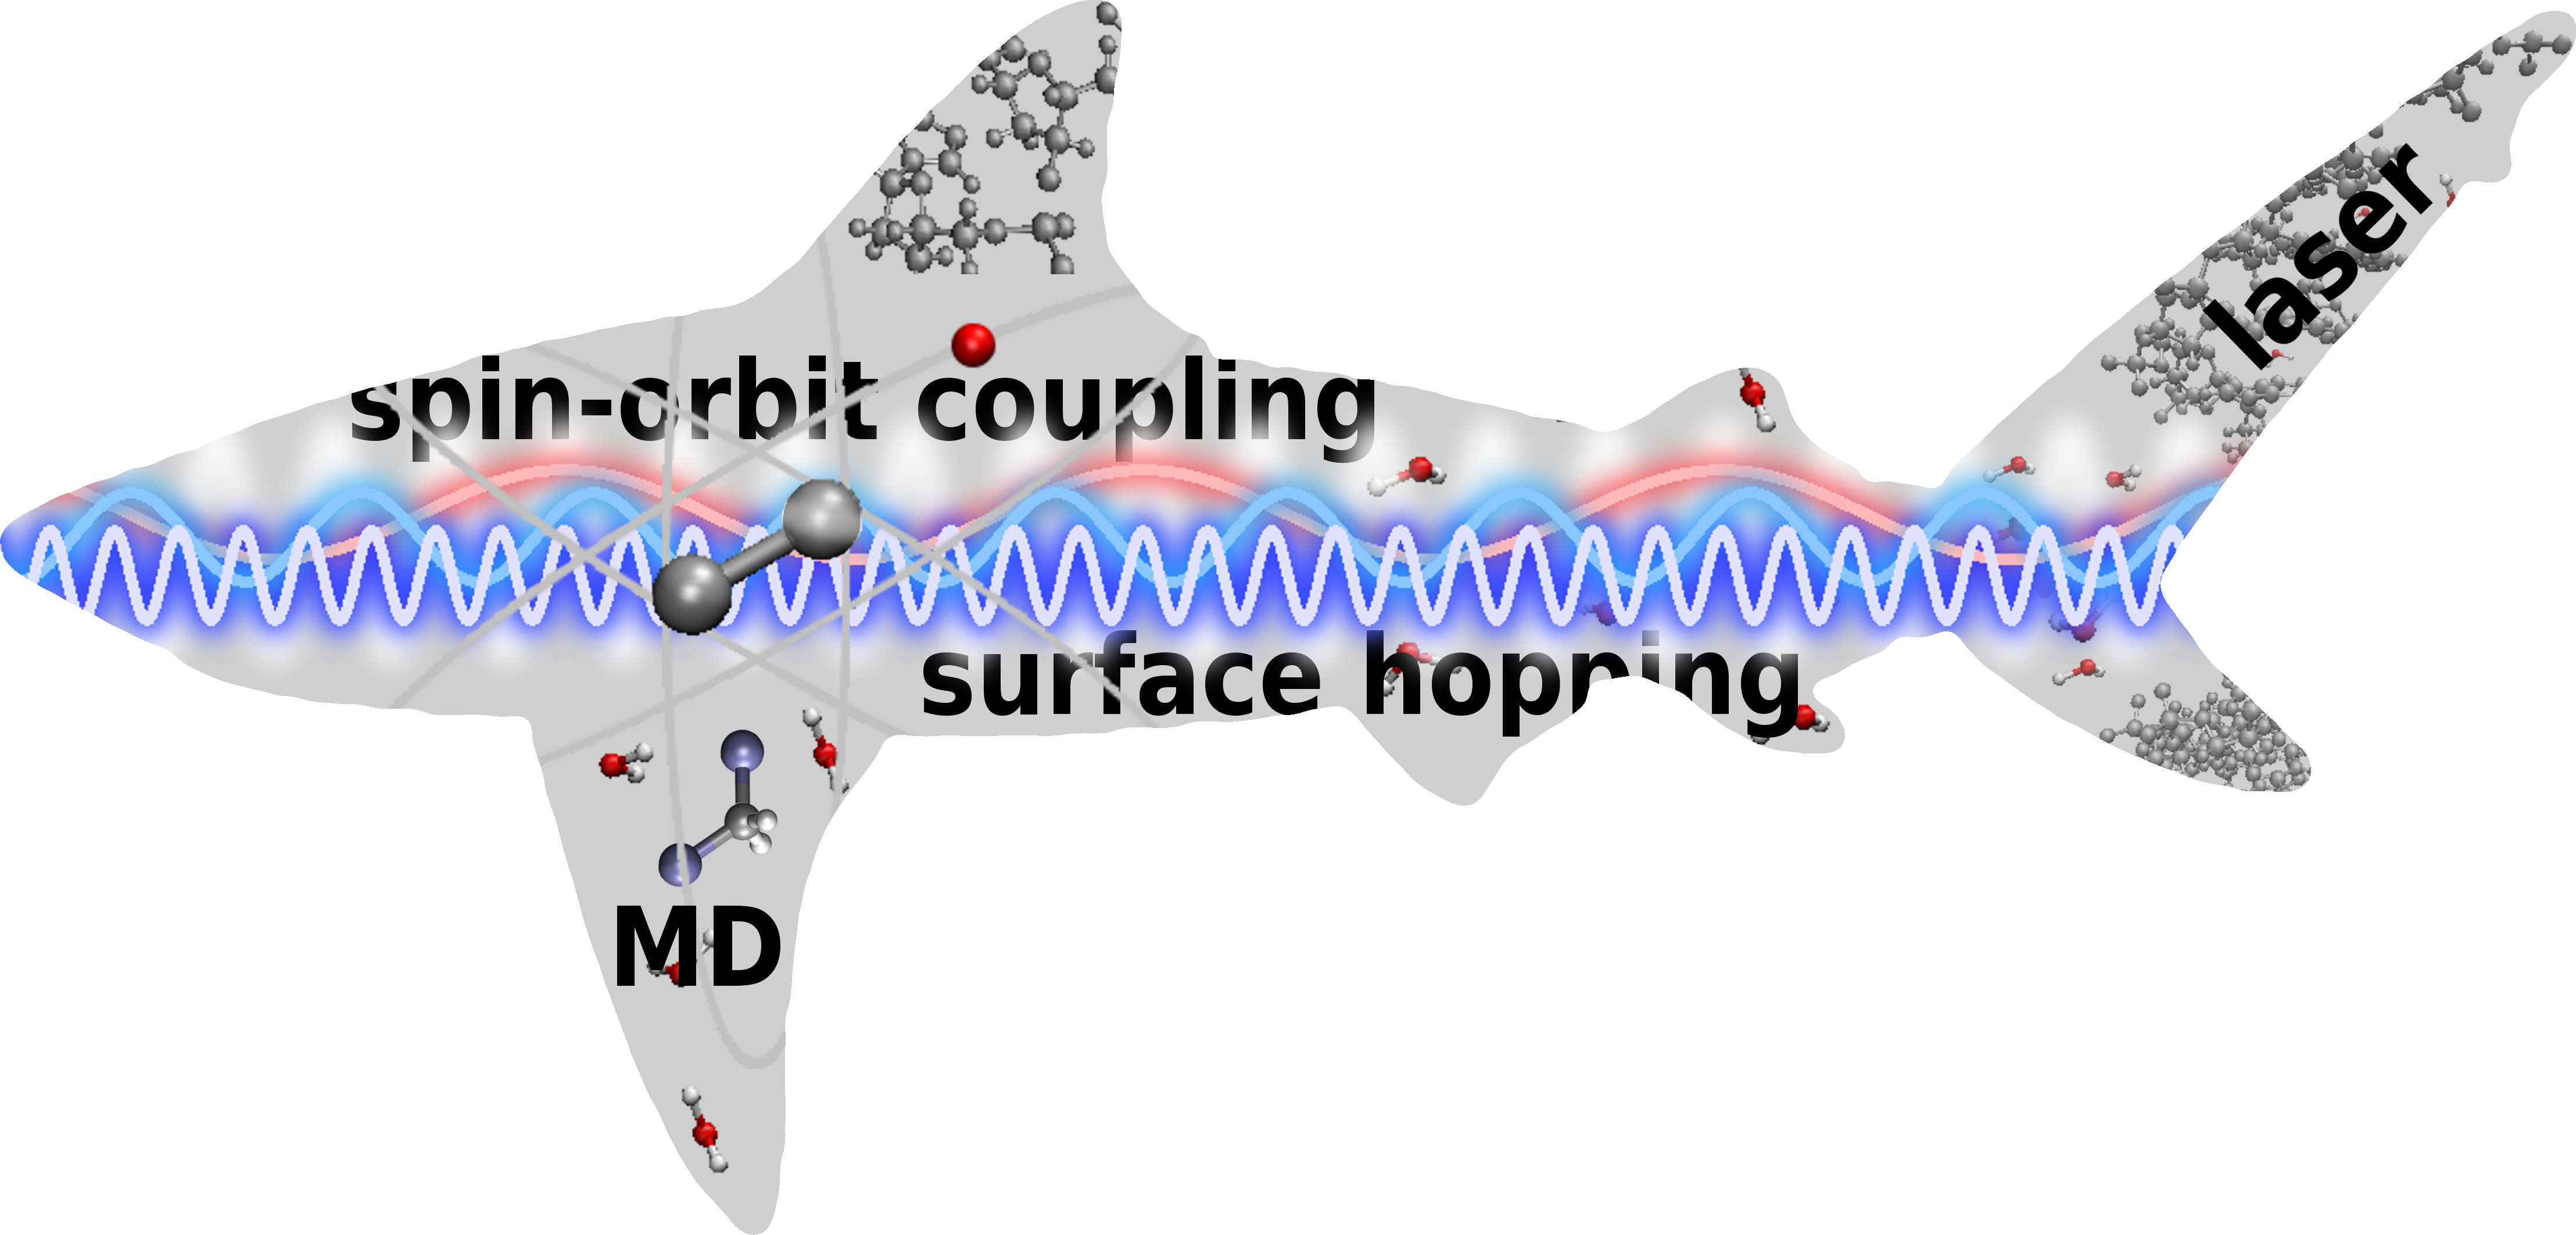
\includegraphics[width=0.8\textwidth,keepaspectratio=true]{img/sharc.png}\vspace{1.5cm}\\
    SHARC: Surface Hopping in the Adiabatic Representation Including Arbitrary Couplings}
    \subtitle{Manual}
    \date{Vienna, \today}
    \author{AG Gonz\'alez\\
Institute of Theoretical Chemistry\\
University of Vienna, Austria
\vspace{1cm}
\\

\includegraphics[width=0.4\textwidth,keepaspectratio=true]{img/univie.pdf}}

    \maketitle
  \end{titlepage}
}{}



% =============================== HEADER AND FOOT ==========================
\tthdump{
  \usepackage[automark]{scrpage2}
  \pagestyle{scrheadings}
  \clearscrheadfoot
}

% \lstset{        numbers=left, 
%                 numberstyle=\tiny, 
%                 numbersep=5pt, 
%                 showstringspaces=true, 
%                 showspaces=false, 
%                 basicstyle=\ttfamily\small, 
%                 commentstyle=\color{black!50},
%                 keywordstyle=\color{B},
%                 stringstyle=\color{red},
%                 fontadjust=false, 
%                 breaklines=true, 
%                 breakatwhitespace=true, 
%                 breakautoindent=true, 
%                 flexiblecolumns=true, 
%                 language=fortran,
%                 morekeywords={dconjg},
%                 morekeywords={=},
%                 morekeywords={*}
%                 }


% =============================== KEYWORDS ==========================

\newcommand{\sharc}{\textsc{Sharc}}

\newcommand{\todo}[1]{\textcolor{RL}{#1}}

\newcommand{\ttt}[1]{\texttt{#1}}

\newcommand{\E}{\ensuremath{\mathrm{e}}}
\newcommand{\I}{\ensuremath{\mathrm{i}}}
\newcommand{\D}{\ensuremath{\mathrm{d}}}
%%tth: \def\vec#1{\ensuremath{\mathbf{#1}}}
\tthdump{
  \renewcommand{\vec}[1]{\ensuremath{\mathbf{#1}}}
}
%%tth: \def\l{l}
%%tth: \def\middle{}
%%tth: \def\mathfrak#1{\mathcal{#1}}
%%tth: \def\ce#1{#1}

% unnumbered things
\newenvironment{unnumbered}%
{\setcounter{secnumdepth}{-1}}
{\setcounter{secnumdepth}{2}}

% shaded boxes
\newenvironment{example}{
  \vspace{0mm}
  \definecolor{shadecolor}{HTML}{BBDDFF}
  \begin{shaded}
  \begin{minipage}{0.9\textwidth}
}{
  \end{minipage}
  \end{shaded}
}
\newcommand\hc[2][black]{\setbox0=\hbox{$#2$}\rlap{\raisebox{.45\ht0}{\textcolor{#1}{\rule{\wd0}{1pt}}}}#2}

% ========================================================================================================= %
% ========================================================================================================= %
% ========================================================================================================= %

\begin{document}

\tpage

%%tth: \Large \textcolor{red}{Due to the limited capabilities of HTML to render complex equations, the reader should consult the \href{http://sharc-md.org}{Manual in PDF format} for correctly displayed equations.}
%%tth: \normalsize

\begin{example}
  \textbf{Contact:}

  \begin{tabular}{ll}
    \\
    \multicolumn{2}{l}{AG Gonz\'alez}\\
    \multicolumn{2}{l}{Institute of Theoretical Chemistry, University of Vienna}\\
    \multicolumn{2}{l}{W\"ahringer Stra\ss{}e 17}\\
    \multicolumn{2}{l}{1090 Vienna, Austria}\\
    \\
    Website: &\href{http://sharc-md.org}{sharc-md.org}\\
    Email: &\href{mailto:philipp.marquetand@univie.ac.at}{philipp.marquetand@univie.ac.at}\\
    Email: &\href{mailto:office@univie.ac.at}{office@univie.ac.at}\\
  \end{tabular}
\end{example}

\newpage
\ihead{\textsc{Sharc} Manual}
\ohead{\rightmark}
\ofoot[\pagemark]{\pagemark}

% ========================================================================================================= %
% ========================================================================================================= %
% ========================================================================================================= %

\tableofcontents
% \layout

% ========================================================================================================= %
% ========================================================================================================= %
% ========================================================================================================= %

\chapter{Introduction}

% what is non-adiabatic dynamics
Dynamics involving radiationless processes in the excited-state manifold of molecules are responsible for many photophysical and photochemical processes. For example, the explanation for Kasha's rule \cite{Kasha1950DFS} is that radiationless transfer from higher excited singlet states to the $S_1$ is faster than fluorescence. This radiationless transfer is called internal conversion (IC). In figure~\ref{fig:jablonski}, radiative and radiationless processes are summarized in a so-called Jab{\l}onski diagram.

\begin{figure}[h]
  \centering
  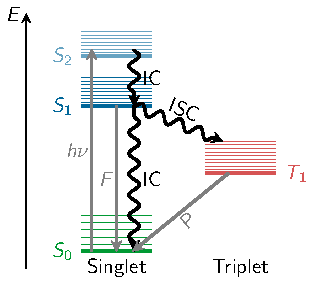
\includegraphics[scale=1.6]{img/jablonski/jablonski.pdf}
  \caption{Jab{\l}onski diagram showing the conceptual photophysical processes. Straight arrows show radiative processes (absorption $h\nu$, fluorescence F, phosphorescence P), wavy arrows show radiationless processes (internal conversion IC and intersystem crossing ISC). }
  \label{fig:jablonski}
\end{figure}

IC also plays a crucial role in the first step of the biological process of visual perception, where the retinal moiety of rhodopsin is hit by a photon and non-radiatively performs a torsion around one of the double bonds, changing the conformation of the protein and inducing a neural signal.
Similarly, protection of the human body from the influence of UV light is achieved through very efficient IC of DNA, proteins and melanins. In these molecules, via ultrafast IC to the electronic ground state, the excitation energy of the UV photons is quickly converted to nuclear kinetic energy, which is spread harmlessly as heat to the environment.
Besides biologically relevant cases, IC processes also occur in the excited-state dynamics of many small molecules, for example \ce{O2} and \ce{O3}, \ce{SO2}, \ce{NO2} and other nitrous oxides, as well as many organic molecules. Hence, these processes are of very high relevance for atmospheric chemistry.

Besides IC, where the system changes between electronic states of the same multiplicity, another important radiationless process is intersystem crossing (ISC), where a change of the electronic spin accompanies the electronic transition. These processes are completely forbidden in the non-relativistic Schr\"odinger equation, but they become allowed when including spin-orbit couplings (SOC), a relativistic effect.
SOC depends on the nuclear charge and becomes stronger for heavy atoms. However, even for molecules with only first- and second-row atoms, ISC might be relevant, for example in \ce{SO2} \cite{Wilkinson2014JCP,Mai2014JCP_SO2,Leveque2014JCP_ISC}, benzene \cite{Penfold2012JCP}, aromatic nitrocompounds \cite{Vogt2013JPC} and DNA nucleobases and derivatives 
\cite{Crespo-Hernandez2004CR, Richter2012JPCL, Mai2013C, Reichardt2010CC}. 

% dynamics simulations
In order to understand those radiationless processes, one of the most important kind of studies employs numeric simulations to follow the nuclear motion on the excited-state potential energy surfaces (PES). These simulations are called excited-state dynamics simulations. Since the Born-Oppenheimer approximation is not applicable for this kind of dynamics, non-adiabatic effects need to be incorporated into the simulations. 

The principal methodology to tackle excited-state dynamics simulations is to numerically integrate the time-dependent Schr\"odinger equation, which is usually called full quantum dynamics simulations (QD). Given accurate PESs, QD is able to reach or surpass experimental accuracy. However, the full multi-dimensional PES is needed for these kinds of simulations, which quickly becomes unfeasible for more than about 6 degrees of freedom. There are several methodologies to overcome this restriction. One of the most popular schemes for non-adiabatic dynamics is the surface hopping methodology.

% surface hopping, advantages, history
Surface hopping was originally devised by Tully \cite{Tully1971JCP, Tully1990JCP}. Since in this manual we can only give a brief theoretical introduction to the topic, we refer to several interesting reviews \cite{Barbatti2011WCMS,Doltsinis2006,Doltsinis2002JTCC}.
In surface hopping, the motion of the excited-state wavepacket is approximated by the motion of an ensemble of many independent, classical trajectories. Each trajectory is at every instant of time tied to one particular PES, and the nuclear motion is integrated using the gradient of this PES. However, non-adiabatic population transfer can lead to the switching of a trajectory from one PES to another PES. This switching (also called ``hopping'', which is the origin of the name ``surface hopping'') is based on a stochastic algorithm, taking into account the change of the electronic population from one timestep to the next one.

The surface hopping methodology's popularity can be explained by a number of advantages \cite{Barbatti2011WCMS}:
\begin{itemize}
  \item The method is conceptually simple, since it is based on classical mechanics. The nuclear propagation is based on Newton's equations and can be performed in cartesian coordinates, avoiding any problems with curved coordinate systems as in QD.
  \item For the propagation of the trajectories only local information of the PESs are needed. This avoids to calculate the full, multi-dimensional PES before the dynamics simulation, which is the main restriction of QD methods. In surface hopping dynamics, all degrees of freedom can be included in the simulation. Additionally, all necessary quantities can be calculated on-demand, usually called ``on-the-fly'' in this context.
  \item The independent trajectories can be trivially parallelized.
\end{itemize}
The strongest of these points of course is the fact that all degrees of freedom can be included easily in the calculations, allowing to describe large systems, like DNA nucleobases, transition metal complexes and even large DNA strands and solvated molecules (by means of QM/MM schemes).
However, the classical nature of the trajectories does not allow to treat some purely quantum-mechanical effects like tunneling, (tunneling for selected degrees of freedom is possible \cite{Hammes-Schiffer1994JCP}). Additionally, quantum coherence between the electronic states is usually described poorly, because of the independent-trajectory ansatz. This can be treated with some ad-hoc corrections, e.g., in \cite{Granucci2007JCP}. 

% SHARC
However, in the original surface hopping method, only non-adiabatic couplings lead to population transfer between different electronic states, allowing only for the description of IC. ISC and radiative processes (absorption) cannot be described, since this necessitates the inclusion of spin-orbit couplings (for ISC) or interactions of dipole moments with electric fields (for absorption). 

The \sharc\ methodology is an extension to standard surface hopping which allows to include these kinds of couplings. The central idea of \sharc\ is to obtain a fully diagonal Hamiltonian, which is adiabatic with respect to all couplings. The diagonal Hamiltonian is obtained by unitary transformation of the Hamiltonian including all couplings. Surface hopping is conducted on the transformed electronic states. 
This has a number of advantages over the standard surface hopping methodology, where no diagonalization is performed:
\begin{itemize}
  \item Potential couplings (like spin-orbit couplings and laser-dipole couplings) are usually delocalized. Surface hopping, however, rests on the assumption that the couplings are localized and hence surface hops only occur in the small region where the couplings are large. Within \sharc\ by transforming the potential couplings away, additional terms of non-adiabatic (kinetic) couplings arise, which are localized. 
  \item The potential couplings have an influence on the gradients acting on the nuclei. To a good approximation, within \sharc\ it is possible to include this influence in the dynamics.
  \item When including spin-orbit couplings for states of higher multiplicity, diagonalization solves the problem of rotational invariance of the multiplet components (see~\cite{Granucci2012JCP}). 
\end{itemize}

A number of methodologies for surface-hopping including different types of potential couplings (similar to \sharc)
have been proposed in references \cite{Granucci2012JCP, Thachuk1996JCP, Maiti2004JPCA,Jones2008JPCA,Mitric2009PRA,Curchod2013C}.

The \sharc\ suite of programs is an implementation of the \sharc\ method. Besides the core dynamics code, it comes with a number of tools, aiding in the setup, maintainance and analysis of the trajectories. 

\section{Capabilities}

Those are the main features of the \sharc\ suite:
\begin{itemize}
  \item Non-adiabatic dynamics based on the surface hopping methodology for internal conversion and intersystem crossing with any number of singlets, doublets, triplets, and higher multiplicities.
  \item Stable propagation in the presence of very small as well as very large spin-orbit couplings.
  \item Inclusion of interactions with laser fields in the long-wavelength limit. The derivatives of the dipole moments can be included in strong-field applications.
  \item Propagation using either non-adiabatic couplings vectors $\langle\alpha|\frac{\partial}{\partial \mathbf{R}}|\beta\rangle$, time-derivative couplings $\langle\alpha|\frac{\partial}{\partial t}|\beta\rangle$ or wavefunction overlaps $\langle\alpha(t_0)|\beta(t)\rangle$ (via the local diabatization procedure \cite{Granucci2007JCP}).
  \item Gradients including the effects of spin-orbit couplings (with the approximation that the diabatic spin-orbit couplings are slowly varying).
  \item Energy-difference-based partial coupling approximation to speed up calculations \cite{Pittner2009CP}.
  \item Energy-based decoherence correction \cite{Granucci2007JCP}.
  \item Calculation of Dyson norms along the trajectories through the \textsc{Columbus} interface.
  \item Flexible interface to quantum chemistry programs. Existing interfaces to \textsc{Molpro}, \textsc{Molcas 7} and \textsc{Columbus 7.1} (only if interfaced to \textsc{Molcas}). An interface to implement dynamics based on analytical expressions is also available.
  \item Suite of auxilliary Python scripts for all steps of the setup procedure and for various analysis tasks.
  \item Comprehensive tutorial.
\end{itemize}

The following features are planned for future versions:
\begin{itemize}
  \item QM/MM calculations.
  \item Dynamics in the Floquet picture.
  \item Description of ionization processes by more advanced methods than Dyson norms.
\end{itemize}


\section{References}

Please cite the following references when using the \sharc\ suite:
{
\newcommand{\enquote}[1]{``#1''}
\begin{example}
  % \begin{itemize}
  %   \item \cite{Mai2014WCMS} \bibentry{Mai2014WCMS}
  % \end{itemize}
  \begin{itemize}
    \item \cite{Richter2011JCTC} \bibentry{Richter2011JCTC}.
    \item \cite{Mai2014SHARC} \bibentry{Mai2014SHARC}.
  \end{itemize}
\end{example}
}

The theoretical background of \sharc\ is described in Refs.~\cite{Richter2011JCTC, Richter2012JCTC_erratum, Bajo2011JPCA, Marquetand2011FD}.

Applications of the \sharc\ code can be found in Refs.~\cite{Richter2012JPCL, Mai2013C, Mai2014TCC, Mai2014JCP_SO2, Gonzalez2014}.

Some features of the \sharc\ suite are described in the following references:
\begin{itemize}
  \item Excited state selection for initial condition generation: \cite{Barbatti2011}.
  \item Energy-based decoherence correction: \cite{Granucci2007JCP}.
  \item Local diabatization and wavefunction overlap calculation: \cite{Granucci2001JCP, Pittner2009CP, Plasser2012JCP}.
  \item Sampling of initial conditions from a quantum-mechanical harmonic Wigner distribution: \cite{Dahl1988JCP, Schinke1995}.
  \item Calculation of ring puckering parameters and their classification: \cite{Cremer1975JACS, Boeyens1976JCMS}.
\end{itemize}

The quantum chemistry programs to which interfaces with \sharc\ exist are described in the following sources:
\begin{itemize}
  \item \textsc{Columbus}: \cite{Lischka2011WCMS, Lischka2012, Yabushita1999JPCA, Mai2014JCP_reindex}.
  \item \textsc{Molpro}: \cite{Werner2012WCMS, Werner2012}.
  \item \textsc{Molcas}: \cite{Karlstrom2003CMS, Aquilante2010JCC}.
\end{itemize}

\section{Authors}

The \sharc\ suite has been programmed by Sebastian Mai and Martin Richter of the AG Gonz\'alez of the Institute of Theoretical Chemistry of the University of Vienna with contributions by Matthias Ruckenbauer, Jes\'us Gonz\'alez-V\'azquez, Philipp Marquetand and Markus Oppel.

\section{Suggestions and Bug Reports}

\begin{example}
Bug reports and suggestions for possible features can be submitted to \href{mailto:philipp.marquetand@univie.ac.at}{philipp.marquetand@univie.ac.at}.
\end{example}

% ========================================================================================================= %
% ========================================================================================================= %
% ========================================================================================================= %

\chapter{Installation}

\section{How To Obtain}

\sharc\ can be obtained from the \sharc\ homepage \href{http://sharc-md.org}{sharc-md.org}. There, click on Download and register with your email adress and affiliation. You will receive a download link via email. Clicking on the link in the email will download the archive file containing the \sharc\ package. Note that the link is active only for 24 h and the number of downloads is limited.

\subsection{Prerequisites}

Note that \sharc\ is only compatible with Linux systems. Windows and OS X are currently not supported. 

In order to carry out ab-initio (CASSCF) on-the-fly dynamics, you will also need one of the following quantum chemistry programs:
\begin{itemize}
  \item \textsc{Molpro} (at least version 2010)
  \item \textsc{Molcas} (at least version 7.8)
\end{itemize}
If you have \textsc{Molcas}, you can also use \textsc{Columbus} (at least 7.1, needs the \textsc{Columbus}-\textsc{Molcas} interface) to carry out dynamics simulations on CASSCF and correlated multi-reference levels (MRCISD, LRT-MRAQCC) of theory.

\section{License}

\begin{example}
Copyright 2014 University of Vienna.

\medskip

Permission is hereby granted, free of charge, to any person obtaining a copy
of this software and associated documentation files (the "Software"), to deal
in the Software without restriction, including without limitation the rights
to use, copy, modify, merge, publish, distribute, sublicense, and/or sell
copies of the Software, and to permit persons to whom the Software is
furnished to do so, subject to the following conditions:

The above copyright notice and this permission notice shall be included in
all copies or substantial portions of the Software.

The Software is provided ``AS IS'', without warranty of any kind, express or
implied, including but not limited to the warranties of merchantability,
fitness for a particular purpose and noninfringement. In no event shall the
authors or copyright holders be liable for any claim, damages or other
liability, whether in an action of contract, tort or otherwise, arising from,
out of or in connection with the software or the use or other dealings in
the Software.
\end{example}

\section{Installation}

The source code of the  \sharc\ suite is distributed as a tar archive file. In order to install it, first extract the content of the archive to a suitable directory.

In order to install and run \sharc, you need the following:
\begin{itemize}
  \item A Fortran90 compiler (Optimally either the \href{https://gcc.gnu.org/fortran/}{GNU Fortran} or the \href{https://software.intel.com/en-us/fortran-compilers}{Intel Fortran} compiler).
  \item The \href{http://www.netlib.org/blas/}{BLAS} and \href{http://www.netlib.org/lapack/}{LAPACK} libraries.
  \item The \href{http://http://www.fftw.org/}{FFTW} package.
  \item \href{https://www.python.org/downloads/release/python-278/}{Python 2 (Version $\geq$2.6)}.
\end{itemize}

To compile the Fortran90 programs of the \sharc\ suite, go to the \ttt{source/} directory and execute \ttt{make}. By default, the \ttt{gfortran} compiler is used. However, by typing \ttt{make intel} instead the \ttt{ifort} compiler will be used. 
It might be necessary to alter the \ttt{LDFLAGS} string in the \ttt{Makefile}, depending on where the BLAS and LAPACK libraries are located on your system.

The FFTW package is only needed if laser fields need to be calculated with \ttt{laser.x}. Dynamics without inclusion of explicit laser fields can be performed without restrictions without the FFTW package.

In order to use the \sharc\ suite, set the environment variable \ttt{\$SHARC} to the \ttt{bin/} directory of the \sharc\ installation. This ensures that all programs of the \sharc\ suite find the other executables and all calls are successful.

Besides the Fortran90 codes, the \sharc\ suite contains a number of Python scripts, most importantly the quantum chemistry interfaces. All Python scripts are written for Python 2 (Version $\geq$2.6) and do not work with Python 3. 

In figure~\ref{fig:installation} the directory structure of the complete \sharc\ directory is shown.

\begin{figure}[h!]
  \centering
  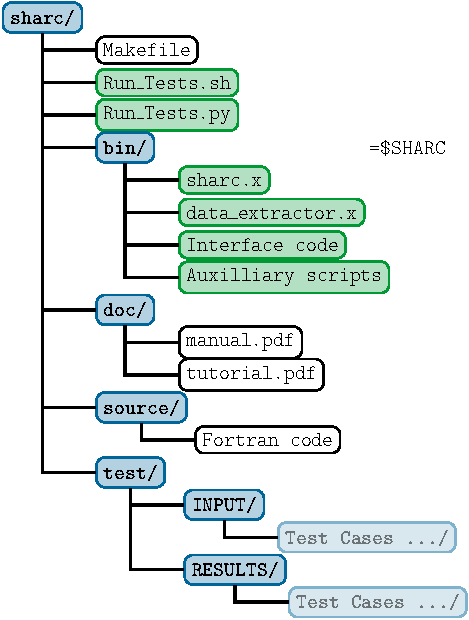
\includegraphics[scale=1]{img/dirs_SHARC/dirs_SHARC.pdf}
  \caption{Directory tree containing a complete \sharc\ installation.}
  \label{fig:installation}
\end{figure}

\subsection{Additional programs}

For full functionality, several additional programs are recommended:
\begin{itemize}
  \item The Python package \href{http://www.numpy.org/}{NumPy}.
  \item The \href{http://www.gnuplot.info/}{\textsc{Gnuplot}} plotting software.
  \item A program for molecular visualization, able to read files in the xyz file format (e.g.\ \href{http://www.cmbi.ru.nl/molden/molden.html}{Molden}, \href{http://gabedit.sourceforge.net/}{Gabedit}, \href{http://molekel.cscs.ch/wiki/pmwiki.php}{Molekel} or \href{http://www.ks.uiuc.edu/Research/vmd/}{VMD})
\end{itemize}

Optimally, within your Python installation the Numpy package should be available. If Numpy is not available, the scripts will fall back to use a small Fortran code (front-end for LAPACK) within the \sharc\ package. Since in the Python scripts no large-scale matrix calculations are carried out, there should be no significant performance loss if Numpy is not available.

\textsc{Gnuplot} is not strictly necessary, since all output files could be plotted using other plotting programs. However, a number of scripts from the \sharc\ suite automatically generate \textsc{Gnuplot} scripts together with the data files.

Even though \sharc\ comes with an interface for analytical potentials (and hence can be used without any quantum chemistry program), the main application of \sharc\ is certainly on-the-fly ab initio dynamics. Hence, one of the following interfaced quantum chemistry programs is necessary:
\begin{itemize}
  \item \href{http://www.molpro.net/}{\textsc{Molpro} 2010 or 2012} (older versions might also work, but this could not be tested).
  \item \href{http://http://molcas.org/}{\textsc{Molcas} 7.8 or 8.0} (older versions of \textsc{Molcas} 7 might also work, but this could not be tested).
  \begin{itemize}
    \item \href{http://www.univie.ac.at/columbus/docs_COL70/documentation_main.html}{\textsc{Columbus} 7}, interfaced to \href{http://http://molcas.org/}{\textsc{Molcas} 7.8} for correlated multi-reference wavefunctions. 
%     \item \href{http://dasher.wustl.edu/tinker/}{Tinker}, interfaced to \textsc{Molcas} 7.8 or 8.0 for QM/MM dynamics.
  \end{itemize}
\end{itemize}


\section{Test Runs}

After the installation is completed, it should be validated. Execute \ttt{\$SHARC/tests.py}, which will first check whether a valid Python version is installed. Afterwards, interactively the user can run the available test simulations. It is recommended to run all tests after the installation (except tests which need quantum chemistry programs the user does not have). 

After the test script has collected all necessary environment variables, the tests are executed. After all tests have been finished, the output files are compared to the reference output, which is part of the \sharc\ package. If any tests reported differing output files, please carefully check the mentioned files. The output files may simply differ in the last decimals for reasons of numerical precision. 

% ========================================================================================================= %
% ========================================================================================================= %
% ========================================================================================================= %

\chapter{Execution}

The \sharc\ suite consists of the main dynamics code \ttt{sharc.x} and a number of auxilliary programs, like setup scripts and analyse tools. Additionally, the suite comes with interfaces to suitable quantum chemistry software, e.g.\ \textsc{Molpro}, \textsc{Molcas} or \textsc{Columbus}. 

In the following, first it is explained how to run a single trajectory by setting up all necessary input for the dynamics code \ttt{sharc.x} manually. Afterwards, the usage of the auxilliary scripts is explained. Detailed infos on the \sharc\ input files is given in chapter~\ref{chap:input} and on the auxilliary scripts in chapter~\ref{chap:aux}. The interfaces are described in chapter~\ref{chap:interfaces}.

\section{Running a single trajectory}

\subsection{Input files}

\sharc\ requires a number of input files, which contain the settings for the dynamics simulation (\ttt{input}), the initial geometry (\ttt{geom}), the initial velocity (\ttt{veloc}), the initial coefficients (\ttt{coeff}) and the laser field (\ttt{laser}). Only the first two (\ttt{input}, \ttt{geom}) are mandatory, the others are optional. The necessary files are shown in figure~\ref{fig:dir_traj}. 
The content of the main input file is explained in detail in section~\ref{sec:inputfile}, the geometry file is specified in section~\ref{sec:geomfile}. The specifications of the velocity, coefficient and laser files are given in sections~\ref{sec:velocfile}, \ref{sec:coefffile} and \ref{sec:laserfile}, respectively.

\begin{figure}[h!]
  \centering
  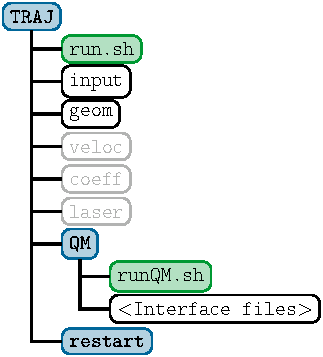
\includegraphics[scale=1]{img/dir_traj/dir_traj.pdf}
  \caption{Input files for a \sharc\ dynamics simulation. Directories are in blue, executable scripts in green, regular files in white and optional files in grey.}
  \label{fig:dir_traj}
\end{figure}

Additionally, the directory \ttt{QM/} and the script \ttt{QM/runQM.sh} need to be present, since the on-the-fly ab initio calculations are implemented through these files. The script \ttt{QM/runQM.sh} is called each time \sharc\ performs an on-the-fly calculation of electronic properties (usually by a quantum chemistry program). In order to do so, \sharc\ first writes the request for the calculation to \ttt{QM/QM.in}, then calls \ttt{QM/runQM.sh}, waits for the script to finish and then reads the requested quantities from \ttt{QM/QM.out}. The script \ttt{QM/runQM.sh} is fully responsible to generate the requested results from the provided input. 
In virtually all cases, this task is handled by the \sharc-quantum chemistry interfaces (see chapter~\ref{chap:interfaces}), so that the script \ttt{QM/runQM.sh} has a particularly simple form:
\begin{example}
  \begin{verbatim}
cd QM/
$SHARC/<INTERFACE> QM.in 
  \end{verbatim}
\end{example}
with the corresponding interface name given. Note that the interfaces in all cases need additional input files, which must be present in \ttt{QM/}. Those input files contain the specifications for the quantum chemistry information, e.g., basis set, active and reference space, memory settings, path to the quantum chemistry program, path to scratch directories; or for \ttt{SHARC\_Analytical.py}, the expressions for the analytical potentials. For each interface, the input files are slightly different. See sections~\ref{sec:int:molpro}, \ref{sec:int:molcas}, \ref{sec:int:columbus} or \ref{sec:int:analytical} for the necessary information.

\subsection{Running the dynamics code}

Given the necessary input files, \sharc\ can be started by executing
\begin{example}
\begin{verbatim}
user@host> $SHARC/sharc.x input
\end{verbatim}
\end{example}
Note that besides the input file, at least the geometry file needs to be present (see in the input section for details).

\subsection{Output files}

Figure~\ref{fig:dir_traj_after} shows the content of a trajectory directory after the execution of \sharc. There will be six new files. These files are \ttt{output.log}, \ttt{output.lis}, \ttt{output.dat} and \ttt{output.xyz}, as well as \ttt{restart.ctrl} and \ttt{restart.traj}.

The file \ttt{output.log} contains mainly a listing of the chosen options and the resulting dynamics settings. At higher print levels, the log file contains also information per timestep (useful for debugging). \ttt{output.lis} contains a table with one line per timestep, giving active states, energies and expectation values. \ttt{output.dat} contains a list of all important matrices and vectors at each timestep. This information can be extracted with \ttt{data\_extractor.x} to yield plottable table files. \ttt{output.xyz} contains the geometries of all timesteps (the comments to each geometry give the active state).
For details about the content of the output files, see chapter~\ref{chap:output}.

The restart files contain the full state of a trajectory and its control variables from the last successful timestep. These files are needed in order to restart a trajectory at this timestep (either because it crashed, or in order to extend the simulation time beyond the original maximum time). 

\begin{figure}[h!]
  \centering
  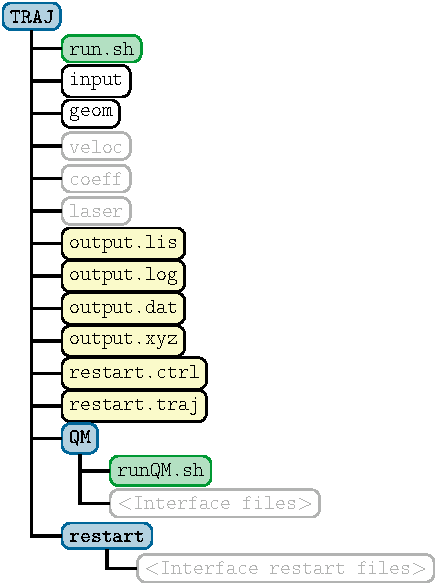
\includegraphics[scale=1]{img/dir_traj/dir_traj_after.pdf}
  \caption{Files of a \sharc\ dynamics simulation after running. Directories are in blue, executable scripts in green, regular files in white and optional files in grey. Output files are in yellow.}
  \label{fig:dir_traj_after}
\end{figure}

\section{Running an ensemble of trajectories}

Usually, one is not interested in running only a single trajectory, since a single trajectory cannot reproduce the branching of a wavepacket into different reaction channels. In order to do so, within surface hopping an ensemble of independent trajectories is employed. 

When dealing with a (possibly large) ensemble of trajectories, setup and analysis need to be automatized. Hence, the \sharc\ suite contains a number of scripts fulfilling different tasks in the usual workflow of setting up ensembles of trajectories.
The typical workflow is given schematically in figure~\ref{fig:workflow}.

\begin{figure}[h!]
  \centering
  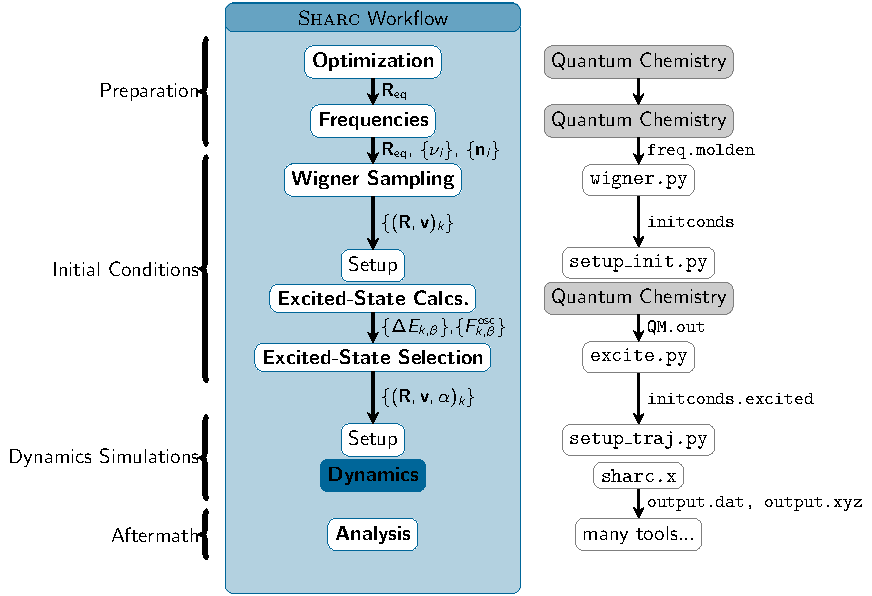
\includegraphics[scale=1]{img/workflow/prepare.pdf}
  \caption{Typical workflow for conducting excited-state dynamics simulations with \sharc.}
  \label{fig:workflow}
\end{figure}

\subsection{Initial condition generation}

In the typical workflow, the user will first create a set of suitable initial conditions. In the context of the \sharc\ package, an initial condition is a set of an initial geometry, initial velocities and initial wavefunction coefficients (together with an initial occupied state). 
A list of many of those sets is needed in order to setup the dynamics simulations.

\paragraph{Initial geometries and velocities}

Currently, within the \sharc\ suite, initial geometries and velocities can be generated based on a quantum harmonic oscillator Wigner distribution. The theoretical background is given in section~\ref{met:wigner}. The calculation is performed by \ttt{wigner.py}, which is explained in section~\ref{sec:wigner.py}. 

As given in figure~\ref{fig:workflow}, \ttt{wigner.py} needs as input the result of a frequency calculation in \textsc{Molden} format. The calculation can be performed by any quantum chemistry program and any method the user sees fit. 
\ttt{wigner.py} produces the file \ttt{initconds}, which contains a list of initial conditions ready for further processing.

\paragraph{Initial coefficients and states}

In the second preparation step, for each of the sampled initial geometries it has to be decided which excited state should be the initial one. This decision is based on a vertical excitation calculation at the same level of theory as in the subsequent dynamics. 

These calculations can be set up with \ttt{setup\_init.py} (see section~\ref{sec:setup_init.py}). This script prepares for each initial condition in the \ttt{initconds} file a directory with the necessary input to perform the calculation. The user should then execute the run script (\ttt{run.sh}) in each of the directories (either manually or through a batch queueing system).

After the vertical excitation calculations are completed, the vertical excitation energies and oscillator strengths of each calculation are collected by \ttt{excite.py} (see~\ref{sec:excite.py}). The same script then performs the selection of the initial electronic state for each initial geometry. The results are written to a new file, \ttt{initconds.excited}. This file contains all information needed to setup the ensemble. Additionally, \ttt{spectrum.py} (\ref{sec:spectrum.py}) can calculate absorption spectra based on the \ttt{initconds.excited} file.

\subsection{Running the dynamics simulations}

Based on the initial conditions given in \ttt{initconds.excited}, the input for all trajectories in the ensemble can be setup by \ttt{setup\_traj.py} (see section~\ref{sec:setup_traj.py}). The script produces one directory for each trajectory, containing the input files for \sharc\ and the selected interface.

In order to run a particular trajectory, the user should execute the run script (\ttt{run.sh}) in the directory of the trajectory. Since those calculations can run for several weeks (depending on the level of theory used and the number of timesteps), it is advisory to submit the run scripts to a batch queueing system. 

The progress of the simulations can be monitored most conveniently in the \ttt{output.lis} files. If the calculations are running in some temporary directory, the output files can be copied to the local directory (where they were setup) with the \ttt{scp} wrapper \ttt{retrieve} (see \ref{sec:retrieve}). This allows to perform ensemble analysis while the trajectories are still running.

If a trajectory crashes, the temporary directory, where the calculation is running, is not deleted. The file \ttt{README} will be created in the trajectory's directory, giving the time of the crash and the location of the temporary data, so that the crash can be investigated. 

\subsection{Analysis of the dynamics results}

Each trajectory can be analyzed independently by inspecting the output files (see chapter~\ref{chap:output}). Most importantly, calling \ttt{data\_extractor.x} (\ref{sec:data_extractor.x}) on the \ttt{output.dat} file of a trajectory creates a number of output files, which can be plotted with the help of \ttt{make\_gnuscript.py} (\ref{sec:make_gnuscript.py}.
The nuclear geometries in \ttt{output.xyz} file can be analyzed efficiently using \ttt{Geo.py} (\ref{sec:Geo.py}).

For the complete ensemble, the script \ttt{populations.py} (section~\ref{sec:populations.py} can calculate average excited-state populations. The script~\ttt{crossing.py} (\ref{sec:crossing.py}) can find and extract notable geometries, e.g., those geometries where a surface hop between two particular states occured.

\section{Auxilliary Programs and Scripts}

The following tables list the auxilliary programs in the \sharc\ suite. The rightmost column gives the section where the program is documented.

\subsection{Setup}

\begin{tabular}{>{\tt}lp{9.5cm}r}
  wigner.py             &Creates initial conditions from Wigner distribution.                   &\ref{sec:wigner.py}\\
  setup\_init.py        &Sets up vertical excitation calculations.                              &\ref{sec:setup_init.py}\\
  excite.py             &Selects initial conditions.                                            &\ref{sec:excite.py}\\
  setup\_traj.py        &Sets up the dynamics simulations based on the initial conditions.      &\ref{sec:setup_traj.py}\\
  molpro\_input.py      &Prepares \textsc{Molpro} input files for common jobs.                  &\ref{sec:molpro_input.py}\\
  molcas\_input.py      &Prepares template files for the \textsc{Molcas} interface.                  &\ref{sec:molcas_input.py}\\
  diagonalizer.x        &Helper program for \ttt{excite.py}. Normally not required.             &\ref{sec:diagonalizer.x}\\
\end{tabular}

\subsection{Analysis}

\begin{tabular}{>{\tt}lp{9.5cm}r}
  retrieve              &\ttt{scp} wrapper to retrieve dynamics output during the simulation.   &\ref{sec:retrieve}\\
  data\_extractor.x     &Extracts plottable results from the \sharc\ output data file.          &\ref{sec:data_extractor.x}\\
  make\_gnuscript.py    &Creates gnuplot scripts for a given number of states.                  &\ref{sec:make_gnuscript.py}\\
  Geo.py                &Calculates internal coordinates from the xyz output file.              &\ref{sec:Geo.py}\\
  populations.py        &Calculates ensemble populations.                                       &\ref{sec:populations.py}\\
  crossing.py           &Extracts specific geometries.                                    &\ref{sec:crossing.py}\\
  spectrum.py           &Generates absorption spectra from initial conditions files.            &\ref{sec:spectrum.py}\\
\end{tabular}

\subsection{Interfaces}

\begin{tabular}{>{\tt}lp{9.5cm}r}
  SHARC\_MOLPRO.py      &Allows for the calculation of SOC, gradients, non-adiabatic couplings, time derivatives, overlaps, dipole moments and angular momentum expectation values at the CASSCF level of theory. Symmetry or RASSCF are not supported. Only segmented basis sets are possible.   &\ref{sec:int:molpro}\\
  SHARC\_MOLCAS.py      &Allows for the calculation of SOC, gradients, overlaps and dipole moments at the CASSCF and RASSCF level of theory. Symmetry is not supported. QM/MM capabilities and trivial parallelization of gradient calculation will be available in the future.         &\ref{sec:int:molcas}\\
  SHARC\_COLUMBUS.py    &Allows for the calculation of SOC, gradients, (non-adiabatic couplings), overlaps, dipole moments and Dyson norms at the CASSCF, RASSCF, MRCISD and LRT-MRAQCC level of theory. Symmetry is not supported. More accurate ionization transition properties will be available in the future. Only works with the \textsc{Columbus}-\textsc{Molcas} interface.                  &\ref{sec:int:columbus}\\
  SHARC\_Analytical.py  &Allows to calculate a 2 singlets + 2 triplets system based on analytical expressions for the diabatic states. Supports up to three dimensions.         &\ref{sec:int:analytical}\\
\end{tabular}



% ========================================================================================================= %
% ========================================================================================================= %
% ========================================================================================================= %

\chapter{Input structure}\label{chap:input}

% \sharc\ is built in a modular way, with a clear separation between the dynamics code and the quantum chemistry software. The connection between these two parts is mediated by the interfaces, which are specific for each quantum chemistry software. The interfaces are described in chapter~\ref{chap:interfaces}. 

In this chapter, the format of all \sharc\ input files are presented. Those are the main input file (called \ttt{input}), the geometry file, the velocity file, the coefficients file and the laser file. Only the first two are necessary, the others are optional input files. All input files are ASCII text files.

% ========================================================================================================= %

\section{Main input file}\label{sec:inputfile}

This section presents the format and all input keywords for the main \sharc\ input. Note that when using \ttt{setup\_traj.py}, full knowledge of the \sharc\ input keywords is not required.

\subsection{General remarks}

The input file has a relatively flexible structure. With very few exceptions, each single line is independent. An input line starts with a keyword, followed optionally by a number of arguments to this keyword. Example:

\begin{example}
  \ttt{stepsize 0.5}
\end{example}

Here, \ttt{stepsize} is the keyword, referring to the size of the timesteps for the nuclear motion in the dynamics. \ttt{0.5} gives the size of this timestep, in this example 0.5~fs.

In each line a trailing comment can be added in the input file, by using the special character \ttt{\#}. Everything after \ttt{\#} is ignored by the input parser of \sharc. The input file also can contain arbitrary blank lines and lines containing only comments. Also, the order of the keywords is completely arbitray. Note however, that if a keyword is repeated in the input only the \textit{first} instance affects the program. Furthermore, note that all input is case-insensitive.

\subsection{Input keywords}

In Table~\ref{tab:input}, all input keywords for the \sharc\ input file are listed.

\clearpage
{
%%tth: \newcommand{\DEFAULT}[1]{\textbf{\textcolor{PineGreen}{#1}}}
\tthdump{
  \newcommand{\DEFAULT}[1]{\textbf{\textcolor{G}{#1}}}
}
\begin{longtable}{|>{\tt}l|l|p{7cm}|}
  \caption{Input keywords. The first column gives the name of the keyword, the second lists possible arguments and the third line provides an explanation. Defaults are marked like \DEFAULT{this}. \$$n$ denotes the $n$-th argument to the keyword.}  \label{tab:input}\\

% ========================================

    \hline
    \rmfamily Keyword     &Arguments    &Explanation\\
    \hline
  \endfirsthead

% ========================================

\tthdump{
    \multicolumn{3}{c}{{\bfseries \tablename\ \thetable{} \mdseries-- Continued from previous page}} \\
    \hline
    \rmfamily Keyword     &Arguments    &Explanation\\
    \hline
  \endhead
}

% ========================================

\tthdump{
    \hline 
    \multicolumn{3}{r}{{Continued on next page}} \\ 
%     \hline
  \endfoot
}
  
% =======================================

\tthdump{
    \hline
  \endlastfoot
}

% ========================================

  printlevel            &\textbf{integer}                    &Controls the verbosity of the log file.\\
                        &\$1=0                               &\footnotesize Log file is empty\\
                        &\$1=1                               &\footnotesize + List of internal steps\\
                        &\$1\DEFAULT{=2}                      &\footnotesize + Input parsing information\\
                        &\$1=3                               &\footnotesize + Some information per timestep\\
                        &\$1=4                               &\footnotesize + More information per timestep\\
                        &\$1=5                               &\footnotesize + Much information per timestep\\
  \hline
  restart               &                                    &Dynamics is resumed from restart files.\\
  \DEFAULT{norestart}    &                                    &Dynamics is initialized from input files.\\
                        &                                    &\footnotesize \ttt{norestart} takes precedence.\\
  \hline
  nstates               &list of \textbf{integer}s           &Number of states per multiplicity.\\
                        &\$1 (\DEFAULT{1})              &\footnotesize Number of singlet states\\
                        &\$2 (\DEFAULT{0})              &\footnotesize Number of doublet states\\
                        &\$3 (\DEFAULT{0})              &\footnotesize Number of triplet states\\
                        &\$\dots (\DEFAULT{0})          &\footnotesize Number of states of higher multiplicities\\
  \hline
  actstates             &list of \textbf{integer}s           &Number of active states per multiplicity.\\
                        &\DEFAULT{same as \ttt{nstates}}     &\footnotesize By default, all states are active.\\
  \hline
  state                 &\textbf{integer}, \textbf{string}   &Specifies the initial state (no default; \sharc\ exits if \ttt{state} is missing).\\
                        &\$1                                 &\footnotesize Initial state.\\
                        &\$2=MCH                             &\footnotesize Initial state and coefficients are given in MCH representation.\\
                        &\$2=diag                            &\footnotesize Initial state and coefficients are given in diagonal representation.\\
  \hline
  coeff                 &\textbf{string}                     &Sets the wavefunction coefficients.\\
                        &\$1\DEFAULT{=auto}                  &\footnotesize Initial coefficient are determined automatically from initial state.\\
                        &\$1=external                        &\footnotesize Initial coefficients are read from file.\\
  \hline
  coefffile             &\textbf{quoted string}              &File containing the initial wavefunction coefficients.\\
                        &\DEFAULT{"coeff"}                   &\\
  \hline
  geomfile              &\textbf{quoted string}              &File name containing the initial geometry.\\
                        &\DEFAULT{"geom"}                    &\\
  \hline
  veloc                 &\textbf{string}                     &Sets the initial velocities.\\
                        &\$1\DEFAULT{=zero}                  &\footnotesize Initial velocities are zero.\\
                        &\$1=random \$2 \textbf{float}       &\footnotesize Initial velocities are determined randomly with \$2 eV kinetic energy per atom.\\
                        &\$1=external                        &\footnotesize Initial velocities are read from file.\\
  \hline
  velocfile             &\textbf{quoted string}              &File containing the initial velocities.\\
                        &\DEFAULT{"veloc"}                   &\\
  \hline
  laser                 &\textbf{string}                     &Sets the laser field.\\
                        &\$1\DEFAULT{=none}                  &\footnotesize No laser field is applied.\\
                        &\$1=internal                        &\footnotesize Laser field is calculated at each timestep from internal function.\\
                        &\$1=external                        &\footnotesize Laser field for each timestep is read during initialization.\\
  \hline
  laserfile             &\textbf{quoted string}              &File containing the laser field.\\
                        &\DEFAULT{"laser"}                   &\\
  \hline
  stepsize              &\textbf{float}                      &Length of the nuclear dynamics timesteps in fs.\\
                        &\DEFAULT{0.5 fs}                    &\\
  \hline
  nsubsteps             &\textbf{integer}                    &Number of substeps for the electronic dynamics.\\
                        &\DEFAULT{25}                        &\\
  \hline
  nsteps                &\textbf{integer}                    &Number of simulation steps.\\
                        &\DEFAULT{3}                         &\\
  \hline
  tmax                  &\textbf{float}                      &Total length of the simulation in fs.\\
                        &                                    &\footnotesize No effect if \ttt{nsteps} is present.\\
  \hline
  killafter             &\textbf{float}                      &Terminates the trajectory after \$1 fs in the lowest state.\\
                        &\DEFAULT{$\infty$}                  &\footnotesize Trajectories are never killed by default.\\
  \hline
  surf                  &\textbf{string}                     &Chooses the potential energy surfaces used in surface hopping.\\
                        &\$1\DEFAULT{=sharc}                 &\footnotesize Uses the diagonal potentials.\\
                        &\$1=fish                            &\footnotesize Uses the MCH potentials.\\
  \hline
  coupling              &\textbf{string}                     &Chooses the quantities describing the non-adiabatic couplings.\\
                        &\$1\DEFAULT{=ddr}                   &\footnotesize Uses vectorial non-adiabatic couplings $\langle\psi_\alpha|\partial/\partial R|\psi_\beta\rangle$.\\
                        &\$1=ddt                             &\footnotesize Uses temporal non-adiabatic couplings $\langle\psi_\alpha|\partial/\partial t|\psi_\beta\rangle$.\\
                        &\$1=overlap                         &\footnotesize Uses the overlaps $\langle\psi_\alpha(t_0)|\psi_\beta(t)\rangle$ (Local Diabatization).\\
  \hline
  gradcorrect           &                                    &Includes $(E_\alpha-E_\beta)\langle\psi_\alpha|\partial/\partial R|\psi_\beta\rangle$ in the gradient transformation.\\
  \DEFAULT{nogradcorrect}&                                    &Transforms only the gradients itself.\\
  \hline
  ekincorrect           &\textbf{string}                     &Adjustment of the kinetic energy after a surface hop.\\
                        &\$1=none                            &\footnotesize Kinetic energy is not adjusted. Jumps are never frustrated.\\
                        &\$1\DEFAULT{=parallel\_vel}         &\footnotesize Velocity is rescaled to adjust kinetic energy.\\
                        &\$1=parallel\_nac                   &\footnotesize Only the velocity component in the direction of $\langle\psi_\alpha|\partial/\partial R|\psi_\beta\rangle$ is rescaled.\\
  \hline
  grad\_select          &                                    &Only some gradients are calculated at every timestep.\\
  \DEFAULT{grad\_all}    &                                    &All gradients are calculated at every timestep.\\
                        &                                    &\footnotesize \ttt{grad\_all} takes precedence.\\
  \hline
  nac\_select           &                                    &Only some $\langle\psi_\alpha|\partial/\partial R|\psi_\beta\rangle$ are calculated at every timestep.\\
  \DEFAULT{nac\_all}     &                                    &All $\langle\psi_\alpha|\partial/\partial R|\psi_\beta\rangle$ are calculated at every timestep.\\
                        &                                    &\footnotesize \ttt{nac\_all} takes precedence.\\
  \hline
  eselect               &\textbf{float}                      &Parameter for selection of gradients and non-adiabatic couplings (in eV).\\
                        &\DEFAULT{0.5 eV}                    &\\
  \hline
  select\_directly      &                                    &Selection of gradients and NACs in one call.\\
  \hline
  ezero                 &\textbf{float}                      &Energy shift for the diagonal elements of the Hamiltonian (in hartree).\\
                        &\DEFAULT{0.0}                       &\footnotesize Is not determined automatically.\\
  \hline
  scaling               &\textbf{float}                      &Scaling factor for the Hamiltonian matrix and the gradients.\\
                        &\DEFAULT{1.0}                       &\footnotesize $0.<$\$1\\
  \hline
  dampeddyn             &\textbf{float}                      &Scaling factor for the kinetic energy at each timestep.\\
                        &\DEFAULT{1.0}                       &\footnotesize $0.\le$\$1$\le1.$\\
  \hline
  rngseed               &\textbf{integer}                    &Seed for the random number generator.\\
                        &\DEFAULT{10997279}                  &\\
  \hline
  decoherence           &                                    &Applies decoherence correction.\\
  \DEFAULT{nodecoherence}&                                    &No decoherence correction.\\
                        &                                    &\footnotesize \ttt{nodecoherence} takes precedence.\\
  \hline
  decoherence\_param    &\textbf{float}                      &The value $\alpha$ in the decoherence correction (in Hartree).\\
                        &\DEFAULT{0.1}                       &\footnotesize $0.<$\$1\\
  \hline
  ionization            &                                    &Calculates ionization probabilities on-the-fly.\\
  \DEFAULT{noionization}&                                    &No ionization probabilities.\\
  \hline
  ionization\_step      &\textbf{integer}                    &Calculates ionization probabilities every \$1 timestep.\\
                        &\DEFAULT{1}                          &By default calculated every timestep (if at all).\\
  \hline
  \DEFAULT{track\_phase}&                                    &Follows the phase of the transformation matrix $\mathbf{U}$.\\
  no\_track\_phase      &                                    &No phase following of $\mathbf{U}$ (not recommended, only for debugging).\\
  \hline
  laserwidth            &\textbf{float}                      &Laser bandwidth used to detect induced hops.\\
                        &\DEFAULT{1.0 eV}                    &\\
  \hline
  dipole\_gradient              &                            &Include the derivatives of the dipole moments in the gradients.\\
  \DEFAULT{nodipole\_gradient}   &                            &Neglect the derivatives of the dipole moments.
\end{longtable}
}

\subsection{Detailed Description of the Keywords}\label{ssec:input:keywords}

\paragraph{Printlevel}

The \ttt{printlevel} keyword controls the verbosity of the log file. The data output file (\ttt{output.dat}) and the listing file (\ttt{output.lis}) are not affected by the printlevel. The printlevels are described in section~\ref{sec:logfile}.

\paragraph{Restart}

There are two keywords controlling trajectory restarting. The keyword \ttt{restart} enables restarting, while \ttt{norestart} disables restart. If both keywords are present, \ttt{norestart} takes precedence. The default is no restart.

When restarting, all control variables are read from the restart file instead of the input file. The only exceptions are \ttt{nsteps} and \ttt{tmax}. In this way, a trajectory which ran for the full simulation time can easily be restarted to extend the simulation time.

\paragraph{Number of States and Active States}

The keyword \ttt{nstates} controls how many states are taken into account in the dynamics. The keyword arguments specify the number of singlet, doublet, triplet, etc.\ states. There is no hard-coded maximum multiplicity in the \sharc\ code, however, some interfaces may restrict the maximum multiplicity. 

Using the \ttt{actstates} keyword, the dynamics can be restricted to some lowest states in each multiplicity. For each multiplicity, the number of active states must not be larger than the number of states. All couplings between the active states and the frozen states are deleted. These couplings include off-diagonal elements in the $H^{\text{MCH}}$ matrix, in the overlap matrix and in the DDT matrix. Freezing states can be useful if transient absorption spectra are to be calculated without increasing computational cost due to the large number of states.

Note that the initial state must not be frozen.

\paragraph{Initial State}

The initial state can be given either in MCH or diagonal representation. The keyword \ttt{state} is followed by an integer specifying the initial state and either the string \ttt{mch} or \ttt{diag}. For the MCH representations, states are enumerated according to the canonical state ordering, see~\ref{met:ordering}. The diagonal states are ordered according to energy. Note that the initial state must be active. 

If the initial state is given in the MCH basis, determination of the initial diagonal state is carried out after the initial QM calculation.

\paragraph{Initial Coefficients}

The initial coefficients can be read from a file. The default filename is \ttt{coeff}, but the filename can be given with the keyword \ttt{coefffile}. Note that the filename has to be enclosed in single or double quotes. The file must contain the real and imaginary part of the initial coefficients, one line per state with no blank lines inbetween. These coefficients are interpreted to be in the same representation as the initial state, i.e.\ the \ttt{state} keyword influences the initial coefficients. For details on the file format, see section~\ref{sec:coefffile}.

Alternatively, the initial coefficients can be determined automatically from the initial state, using \ttt{coeff auto} in the input file. If the initial state is given in the diagonal representation as $i$, the initial coefficients are $c^{\text{diag}}_j=\delta_{ij}$. If the initial state is, however, given in the MCH representation, then $c^{\text{MCH}}_j=\delta_{ij}$ and the determination of $\vec{c}^{\text{diag}}=\vec{U}^\dagger\vec{c}^{\text{MCH}}$ is carried out after the initial QM calculation. 

\paragraph{Geometry Input}

The initial geometry must be given in a second file in the same input format which is also used in the \href{http://www.univie.ac.at/columbus/docs_COL70/documentation_main.html}{\textsc{Columbus} geometry file format}. The default name for this file is \ttt{geom}. The geometry filename can be given in the input file with the \ttt{geomfile} keyword. Note that the filename has to be enclosed in single or double quotes. See section~\ref{sec:geomfile} for more details.

\paragraph{Velocity Input}

Using the \ttt{veloc} keyword, the initial velocities can be either set to zero, determined randomly or read from a file. Random determination of the velocities is such that each atom has the same kinetic energy, which must be specified after \ttt{veloc random} in units of eV. Determination of the random velocities is detailed in~\ref{met:veloc}.

Alternatively, the initial velocities can be read from a file. 
The default velocity filename is \ttt{veloc}, but the filename can be specified with the \ttt{velocfile} keyword. Note that the filename has to be enclosed in single or double quotes. The file must contain the cartesian components of the velocity for each atom on a new line, in the same order as in the geomety file. The velocity is interpreted in terms of atomic units (bohr/atu). See section~\ref{sec:velocfile} for more details.

\paragraph{Laser Input}

The keyword \ttt{laser} controls whether a laser field is included in the dynamics (influencing the coefficient propagation and the energies/gradients by means of the Stark effect). 

The input of an external laser field uses the file \ttt{laser}. This file is specified in \ref{sec:laserfile}.

\paragraph{Laser Width}

In order to detect laser-induced hops, \sharc\ compares the instantaneous central laser energy with the energy gap between the old and new states. If the difference between the laser energy and the energy gap is smaller than the laser bandwidth, the hop is classified as laser-induced. Those hops are never frustrated and the kinetic energy is not scaled to preserve total energy (instead, the kinetic energy is preserved).

\paragraph{Simulation Timestep}

The keyword \ttt{stepsize} controls the length of a timestep (in fs) for the dynamics. The nuclear motion is integrated using the Velocity-Verlet algorithm with this timestep. Surface hopping is performed once per timestep and 1--3 quantum chemistry calculations are performed per timestep (depending on the selection schedule). Each timestep is divided in \ttt{nsubsteps} substeps for the integration of the electronic equation-of-motion. Since integration is performed in the MCH representation, the default of 25 substeps is usually sufficient, even if very small potential couplings are encountered.

\paragraph{Simulation Time}

The keyword \ttt{nsteps} controls the total length of the simulation. The total simulation time is \ttt{nsteps} times \ttt{stepsize}. \ttt{nsteps} does not include the initial quantum chemistry calculation. Instead of the number of steps the total simulation time can be given directly (in fs) using the keyword \ttt{tmax}. In this case, \ttt{nsteps} is calculated as \ttt{tmax} divided by \ttt{stepsize}. If both keywords (\ttt{nsteps} and \ttt{tmax}) are present, \ttt{nsteps} is used.

Using the keyword \ttt{killafter}, the dynamics can be terminated before the full simulation time. \ttt{killafter} specifies (in fs) the time the trajectory can move in the lowest-energy state before the simulation is terminated. By default, simulations always run to the full simulation time and are not terminated prematurely.

\paragraph{Surface Treatment}

The keyword \ttt{surf} controls whether the dynamics runs on diagonal potential energy surfaces (which makes it a \sharc\ simulation) or on the MCH PESs (which corresponds to a \textsc{Fish} simulation). Internally, a \textsc{Fish} simulation is conducted by setting the $U$ matrix equal to the unity matrix at each timestep. 

\paragraph{Description of Non-adiabatic Coupling}

The code allows to propagate the electronic wavefunction using three different quantities describing non-adiabatic effects, see~\ref{met:propagate}. The keyword \ttt{coupling} controls which of these quantities is requested from the QM interfaces and used in the propagation. The default is \ttt{ddr}, which requests the non-adiabatic coupling vectors $\langle\psi_\alpha|\partial/\partial \vec{R}|\psi_\beta\rangle$. For the wavefunction propagation, the scalar product of these vectors and the nuclear velocity is calculated to obtain the matrix $\langle\psi_\alpha|\partial/\partial t|\psi_\beta\rangle$. During the propagation, this matrix is interpolated linearly.

Alternatively, some interfaces can directly calculate the matrix elements $\langle\psi_\alpha|\partial/\partial t|\psi_\beta\rangle$, which can be used for the propagation. The corresponding argument to \ttt{coupling} is \ttt{ddt}. In this case, the matrix is taken as constant during the integration.

The third possibility is the use of the overlap matrix, requested with \ttt{coupling overlaps}. The overlap matrix is used subsequently in the Local Diabatization algorithm for the wavefunction propagation.

\paragraph{Decoherence}

Decoherence according to Granucci et al.\cite{Granucci2010JCP} can be applied to the diagonal coefficients by using the keyword \ttt{decoherence}. By default, decoherence is off. The keyword \ttt{nodecoherence} turns decoherence off. 

The keyword \ttt{decoherence\_param} can be used to change the parameter $\alpha$ (see~\ref{met:decoherence}). The default is 0.1~Hartree, which is the value recommended by Granucci et al.

\paragraph{Correction to the Gradients}

As detailed in~\ref{met:gradtra}, the correct transformation of the gradients to the diagonal representation includes contributions from the non-adiabatic coupling vectors. Using \ttt{gradcorrect true}, these contributions are included. In this case \sharc\ will request the calculation of the non-adiabatic coupling vectors, even if they are not used in the wavefunction propagation. 

\paragraph{Dipole Moment Gradients}

As explained in~\ref{met:dipolegrad}, the derivatives of the dipole moments can be included in the gradients. This can be activated with the keyword \ttt{dipole\_gradient}. Currently, only the analytical interface can deliver these quantities.

\paragraph{Frustrated Hops and Adjustment of the Kinetic Energy}

The keyword \ttt{ekincorrect} controls how the kinetic energy is adjusted after a surface hop to preserve total energy. \ttt{ekincorrect none} deactivates the adjustment, so that the total energy is not preserved after a hop. Using this option, jumps can never be frustrated and are always performed according to the hopping probabilities. 
Using \ttt{ekincorrect parallel\_vel}, the kinetic energy is adjusted by simply rescaling the nuclear velocities so that the new kinetic energy is $E_{\text{tot}}-E_{\text{pot}}$. Jumps are frustrated if the new potential energy would exceed the total energy.
Finally, using \ttt{ekincorrect parallel\_nac}, the kinetic energy is adjusted by rescaling the component of the nuclear velocities parallel to the non-adiabatic coupling vector between the old and new state. The hop is frustrated if there is not enough kinetic energy in this direction to conserve total energy. Note that \ttt{ekincorrect parallel\_nac} implies the calculation of the non-adiabatic coupling vector, even if they are not used for the wavefunction propagation.

\paragraph{Selection of Gradients and Non-Adiabatic Couplings}

\sharc\ allows to selectively calculate only certain gradients and non-adiabatic coupling vectors at each timestep. Those gradients and non-adiabatic coupling vectors not selected are not requested from the interfaces, thus decreasing the computational cost. The selection procedure is detailed in~\ref{met:selection}.
Selection of gradients is activated by \ttt{grad\_select}, selection for non-adiabatic couplings by \ttt{nac\_select}. Selection is turned off by default. 

The selection procedure picks only states which are closer in energy to the classically occupied state than a given threshold. The threshold is 0.5~eV by default and can be adjusted using the \ttt{eselect} keyword.

By default, if \sharc\ performs such selection it will do two quantum chemistry calls per timestep. In the first call, all quantities are requested except for the ones to be selected. The energies are used to determine which gradients and NACs to calculate. The keyword \ttt{select\_directly} tells \sharc\ instead to use the energies of the last timestep, so that only one call per timestep is necessary.

\paragraph{Ionization}

The keyword \ttt{ionization} activates the on-the-fly calculation of ionization transition properties. If the keyword is given, by default these properties are calculated every timestep. The keyword \ttt{ionization\_step} can be used to calculate these properties only every $n$-th timestep. 
If the keyword is given, \sharc\ will request the calculation of the ionization properties from the interface, which needs to be able to calculate them (currently only the \textsc{Columbus} interface can perform these calculations).

\paragraph{Phase Tracking}

Using the keywords \ttt{track\_phase} and \ttt{no\_track\_phase}, the tracking of the eigenvector phases of the transformation matrix $\mathbf{U}$ (see \ref{met:phase_track}) can be switched on or off. However, it is usually not a good idea to deactivate the phase tracking, since this might lead to spurious behaviour in the wavefunction propagation and the surface hopping.


\subsection{Example}

The following input sample shows a typical input for excited-state dynamics including IC within a singlet manifold plus intersystem crossing to triplet states. It includes a large number of excited singlet states in order to calculate transient absorption spectra. Only the lowest three singlet states actually participate in the dynamics. 

\begin{example}
  \begin{verbatim}
  nstates   8 0 3       # many singlet states for transient absorption
  actstates 3 0 3       # only few states to reduce cost

  stepsize 0.5          # typical timestep for a molecule containing H
  tmax 1000.0           # one ps

  surf sharc
  state 3 mch                  # start on the S2 singlet state
  coeff auto                   # coefficient of S2 will be set to one
  coupling ddr                 # \
  decoherence                  # | typical settings
  ekincorrect parallel_vel     # /
  grad_select           # \
  nac_select            # | improve performance
  eselect 0.3           # /

  veloc external        # velocity comes from file "veloc"
  velocfile "veloc"     #

  RNGseed 65435
  ezero -399.41494751   # ground state energy of molecule
  \end{verbatim}
\end{example}



\section{Geometry file}\label{sec:geomfile}

The geometry file (default file name is \ttt{geom}) contains the initial coordinates of all atoms. This file must be present when starting a new trajectory.

It uses the \href{http://www.univie.ac.at/columbus/docs_COL70/documentation_main.html}{\textsc{Columbus} geometry file format}. For each atom, the file contains one line, giving the chemical symbol (a string), the atomic number (a real number), the $x$, $y$ and $z$ coordinates of the atom in Bohrs (three real numbers), and the relative atomic weight of the atom (a real number). The six items must be separated by spaces. The real numbers are read in using Fortran list-directed I/O, and hence are free format (can have any numbers of decimals, exponential notation, etc.). Element symbols can have at most 2 characters.

The following is an example of a \ttt{geom} file for \ce{CH2}:
\begin{example}
  \begin{verbatim}
C 6.0  0.0 0.0  0.0 12.000
H 1.0  1.7 0.0 -1.2  1.008
H 1.0  1.7 0.0  3.7  1.008
  \end{verbatim}
\end{example}

\section{Velocity file}\label{sec:velocfile}

The velocity file (default \ttt{veloc}) contains the initial nuclear velocities (e.g., from a Wigner distribution sampling). This file is optional (the velocities can be initialized with the \ttt{veloc} input keyword). 

The file contains one line of input for each atom, where the order of atoms must be the same as in the \ttt{geom} file. Each line consists of three items, separated by spaces, where the first is the $x$ component of the nuclear velocity, followed by the $y$ and $z$ components (three real numbers). The input is interpreted in atomic units (Bohr/atu).

The following is an example of a \ttt{veloc} file:
\begin{example}
  \begin{verbatim}
 0.0001  0.0000  0.0002
-0.0002  0.0000  0.0012
-0.0003  0.0000 -0.0007
  \end{verbatim}
\end{example}

\section{Coefficient file}\label{sec:coefffile}

The coefficient file contains the initial wavefunction coefficients. The file contains one line per state (total number of states, i.e., multiplets count multiple times). Each line specifies the initial coefficient of one state. If the initial state is specified in the MCH representation (input keyword \ttt{state}), then the order of the initial coefficients must be as given by the canonical ordering (see section~\ref{met:ordering}). If the initial state is given in diagonal representation, then the initial coefficients correspond to the states given in energetic ordering, starting with the lowest state.
Each line contains two real numbers, giving first the real and then the imaginary part of the initial coefficient of the respective state.

Example:
\begin{example}
  \begin{verbatim}
0.0 0.0
1.0 0.0
0.0 0.0
  \end{verbatim}
\end{example}

\section{Laser file}\label{sec:laserfile}

The laser file contains a table with the amplitude of the laser field $\boldsymbol{\epsilon}(t)$ at each timestep of the \textit{electronic} propagation. Given a laser field of the general form:
%%tth: \newline\includegraphics{equations/equation_1.gif}\newline
\tthdump{
  \begin{equation}
    \boldsymbol{\epsilon}(t)=
    \begin{pmatrix}
      \Re(\epsilon_x(t))+\I \Im(\epsilon_x(t))\\
      \Re(\epsilon_y(t))+\I \Im(\epsilon_y(t))\\
      \Re(\epsilon_z(t))+\I \Im(\epsilon_z(t))
    \end{pmatrix}
  \end{equation}
}
each line consists of 8 elements: $t$ (in fs), $\Re(\epsilon_x(t))$, $\Im(\epsilon_x(t))$, $\Re(\epsilon_y(t))$, $\Im(\epsilon_y(t))$, $\Re(\epsilon_z(t))$, $\Im(\epsilon_z(t))$, (all in atomic units), and finally the instantaneous central frequency (also atomic units).

The timestep in the laser file must exactly match the timestep used for the electronic propagation, which is the timestep used for the nuclear propagation (keyword \ttt{stepsize}) divided by the number of substeps (keyword \ttt{nsubsteps}). The first line of the laser file must correspond to $t$=0 fs.

\chapter{Output files}\label{chap:output}

This chapter documents the content of the output files of \sharc. Those output files are \ttt{output.log}, \ttt{output.lis}, \ttt{output.dat} and \ttt{output.xyz}.

\section{Log file}\label{sec:logfile}

The log file \ttt{output.log} contains general information about all steps of the \sharc\ simulation, e.g., information about the parsing of the input files, results of quantum chemistry calls, internal matrices and vectors, etc. The content of the log file can be controlled with the keyword \ttt{printlevel} in the \sharc\ main input file.

In the following, all printlevels are explained.

\paragraph{Printlevel 0}

At printlevel 0, only the execution infos (date, host and working directory at execution start) and build infos (compiler, date, building host and working directory) are given.

\paragraph{Printlevel 1}

At printlevel 1, also the content of the input file (cleaned of comments and blank lines) is echoed in the log file. Also, the start of each timestep is given.

\paragraph{Printlevel 2}

At printlevel 2, the log file also contains information about the parsing of the input files (echoing all enabled options, initial geometry, velocity and coefficients, etc.) and about the initialization of the coefficients after the first quantum chemistry calculation. This printlevel is recommended, since it is the highest printlevel where no output per timestep is written to the log file.

\paragraph{Printlevel 3}

This and higher printlevels add output per timestep to the log file. At printlevel 3, the log file contains at each timestep the data from the velocity-Verlet algorithm (old and new acceleration, velocity and geometry), the old and new coefficients, the surface hopping probabilities and random number, the occupancies before and after decoherence correction as well as the kinetic, potential and total energies.

\paragraph{Printlevel 4}

At printlevel 4, additionally the log file contains information on the quantum chemistry calls (file names, which quantities were read, gradient and non-adiabatic coupling vector selection) and the propagator matrix.

\paragraph{Printlevel 5}

At printlevel 5, additionally the log file contains the results of each quantum chemistry calls (all matrices and vectors), all matrices involved in the propagation as well as the matrices involved in the gradient transformation. This is the highest printlevel currently implemented.

\section{Listing file}\label{sec:lisfile}

The listing file \ttt{output.lis} is a tabular summary of the progress of the dynamics simulation. At the end of each timestep (including the initial calculations), one line with 11 elements is printed. These are, from left to right, the current step (counting starts at zero for the initial step), the current simulation time (fs), the current state in the diagonal representation, the approximate corresponding MCH state (see subsection~\ref{ssec:state_transform}, the kinetic, potential and total energy (in eV), the current gradient (in eV/\AA), the current expectation values of the state dipole moment and spin, as well as the wallclock time needed for the timestep.

The listing file also contains one extra line for each surface hopping event. The accepted hops, the old and new states (in diagonal representation) and the random number are given. Frustrated hops and resonant hops are also mentioned. Note that the extra line for surface hopping occurs before the regular line for the timestep. 

The listing file can be plotted with standard tools like \textsc{Gnuplot}. 

\paragraph{Energies}

The kinetic energy is calculated after any surface hopping events and the corresponding adjustment of the kinetic energy. The potential energy is the energy of the currently active diagonal state. The total energy is the sum of those two.

\paragraph{Expectation values}

The gradient given in the listing file is calculated as follows:
\begin{equation}
  g_\text{list}=\sqrt{\frac{1}{3N_\text{atom}}\sum\limits_a^{N_\text{atom}}\sum_{d=x,y,z} g_{ad}^2}
\end{equation}
which is then transformed to eV/\AA.

The expectation values of the dipole moment for the active state $\beta$ is calculated from:
\begin{equation}
  \mu=\sqrt{\sum\limits_{p=x,y,z} 
  \left(
    \sum\limits_\sigma\sum\limits_\tau
    \Re\left[
      U_{\beta\sigma}^\dagger \mu_{\sigma\tau}^p U_{\tau\beta}
    \right]
  \right)^2}
\end{equation}

The expectation value of the total spin of the active state $\beta$ is calculated as follows:
\begin{equation}
  S=\sum_\alpha |U_{\alpha\beta}|^2 S_\alpha
\end{equation}
where $S_\alpha$ is the total spin of the MCH state with index $\alpha$.

\section{Data file}\label{sec:datfile}

The data file \ttt{output.dat} contains all relevant data from the simulation for all timesteps, in ASCII format. Accordingly, this file can become quite large for long trajectories or if many states are included, but for most computer architectures it is easier to deal with a single large file than with many small files.

Usually, after the simulation is finished the data file is processed by \ttt{data\_extractor.x} to obtain a number of tabular files which can be plotted. For this, see sections~\ref{sec:diagonalizer.x} for the data extractor and~\ref{sec:make_gnuscript.py} for plotting.

\subsection{Specification of the data file}

The data file contains a short header followed by the data per timestep. All quantities are commented in the data file.

The header contains the maximum multiplicity, the number of states per multiplicity, the number of atoms, the timestep and energy shift. It also contains flags telling whether overlap matrices are calculated or a laser field is included, the number of steps and number of substeps.

The entry for each timestep contains the step index, the Hamiltonian in MCH representation, the transformation matrix $\vec{U}$, the MCH dipole moment matrices ($x$, $y$, $z$), the overlap matrix in MCH representation (only if used, e.g., for trajectories using local diabatization, see~\ref{met:propagate}), the diagonal coefficients, the diagonal hopping probablities, the kinetic energy, the currently active state in diagonal representation and the approximate state in MCH representation, the random number for surface hopping, as well as geometry (Bohrs) and velocities (atomic units). Additionally, the property matrix is given for each timestep.

\section{XYZ file}\label{sec:xyzfile}

The file \ttt{output.xyz} contains the geometries of all timesteps in standard xyz file format. It can be used with visualization programs like \textsc{Molden}, \textsc{Gabedit} or \textsc{Molekel} to create movies of the molecular motion, or with \ttt{Geo.py} (see~\ref{sec:Geo.py}) to calculate internal coordinates for each timestep.

The comments of the geometries (given in the second line of each geometry block) contain information about the simulation time and the active state (first in diagonal basis, then in MCH basis).


% ========================================================================================================= %
% ========================================================================================================= %
% ========================================================================================================= %

\chapter{Interfaces}\label{chap:interfaces}

% ========================================================================================================= %

\section{Interface Specifications}

The main \sharc\ code is written to work together with any quantum chemistry program, via external interfaces. 

From the \sharc\ side, quantum chemical calculation proceeds as follows in the \ttt{QM} directory:
\begin{enumerate}
  \item write a file called \ttt{QM/QM.in}
  \item call a script called \ttt{QM/runQM.sh}
  \item read the output from a file called \ttt{QM/QM.out}
\end{enumerate}
For specifications of the formats of these two files (\ttt{QM.in} and \ttt{QM.out}) see below. The executable script \ttt{QM/runQM.sh} must accomplish that all necessary quantum chemical output is available in \ttt{QM/QM.out}.

\subsection{\ttt{QM.in} Specification}\label{intf:qmin}

The \ttt{QM.in} file is written by \sharc\ every time a quantum chemistry calculation is necessary. It contains all information available to \sharc. This information includes the current geometry (and velocity), the timestep, the number of states, the timestep and the unit used to specify the atomic coordinates. The file also contains control keywords and request keywords. 

The file format is consistent with a standard xyz file. The first line contains the number of atoms, the second line is a comment. \sharc\ writes the trajectory ID to this line. The following lines specify the atom positions. As a fourth, fifth and sixth column, these lines may contain the atomic velocities.
All following lines contain keywords, one per line and possibly with arguments. Comments can be inserted with '\#', and empty lines are permissible. Comments and empty lines are only permissible below the xyz file part.
An examplary \ttt{QM.in} file is given in the following:
\begin{example}
  \begin{verbatim}
    3
    Jobname
    S     0.0     0.0     0.0    0.000  -0.020   0.002
    H     0.0     0.9     1.2    0.000  -0.030   0.000
    H     0.0    -0.9     1.2    0.000   0.010  -0.000
    # This is a comment
    Init
    States 3 0 2
    Unit Angstrom
    SOC
    DM
    GRAD 1 2
    OVERLAP
    NACDR select
      1 2
      end
  \end{verbatim}
\end{example}

It is distinguished between two types of keywords, control keywords and request keywords. Control keywords pass some information to the interface. Request keywords tell the interface to provide a quantity in the \ttt{QM.out} file.

\paragraph{Control Keywords}

Control keywords tell the interface how to perform the calculations.

\begin{tabular}{lp{9cm}}
init            &Specifies that this is the first calculation. The interface should create a save directory to save all information necessary for a restart. \\
% restart         &\\
samestep        &Specifies that this is an additional calculation at the same geometry/timestep. \\
cleanup         &Specifies that all output files of the interface (except \ttt{QM.out}) should be deleted (including the save directory).\\
unit            &Specifies in which unit the atomic coordinates are to be interpreted. Possible arguments are ``angstrom'' and ``bohr''.\\
states          &Gives the number of excited states per multiplicity (singlets, doublet, triplets, ...).\\
dt              &Gives the time between the last calculation and the current calculation in atomic units.\\
savedir         &Gives a path to the directory where the interface should save files needed for restart and between timesteps. If the interface-specific input files also have this keyword, the path in \ttt{QM.in} must take precedence.\\
\end{tabular}


\paragraph{Request Keywords}

Request keywords tell the interface which calculations to conduct.

\begin{tabular}{lp{9cm}}
H               &Calculate the molecular Hamiltonian (diagonal matrix with the energies of the states of the model space).\\
SOC             &Calculate the molecular Hamiltonian including the SOCs (not diagonal anymore within the model space).\\
DM              &Calculate the state dipole moments and transition dipole moments between all states.\\
ION             &Calculate transition properties between neutral and ionic wavefunctions.\\
GRAD            &Calculate gradients for all states. If followed by a list of states, calculate only gradients for the specified states.\\
NACDT           &Calculate the time-derivatives $\left\langle\Psi_1|\partial/\partial t|\Psi_2\right\rangle$ by finite differences between the last timestep and the current timestep\\
NACDR           &Calculate non-adiabatic coupling vectors $\left\langle\Psi_1|\partial/\partial \mathbf{R}|\Psi_2\right\rangle$ between all pairs of states. If followed by ``select'', read the list of pairs on the following lines until ``end'' and calculate non-adiabatic coupling vectors between the specified pairs of states.\\
OVERLAP         &Calculate overlaps $\left\langle\Psi_1(t_0)|\Psi_2(t)\right\rangle$ between all pairs of states (between the last and current timestep). If followed by ``select'', read the list of pairs on the following lines until ``end'' and calculate overlaps between the specified pairs of states.\\
DMDR            &Calculate the cartesian gradients of the dipole moments and transition dipole moments of all states.\\
\end{tabular}

\subsection{\ttt{QM.out} Specification}\label{intf:qmout}

The \ttt{QM.out} file communicates back the results of the quantum chemistry calculation to the dynamics code. After \sharc\ called \ttt{QM/runQM.sh}, it expects that the file \ttt{QM/QM.out} exists and contains the relevant data.

The following quantities are expected in the file (depending whether the corresponding keyword is in the \ttt{QM.in} file): Hamiltonian matrix, dipole matrices, gradients, non-adiabatic couplings (either NACDR or NACDT), overlaps, wavefunction phases, property matrices. The format of \ttt{QM.out} is described in the following. 

Each quantity is given as a data block, which has a fixed format. The order of the blocks is arbitrary, and between blocks arbitrary lines can be written. However, within a block no extraneous lines are allowed. Each data block starts with a exclamation mark \ttt{!}, followed by whitespace and an integer flag which specifies the type of data:

\begin{tabular}{ll}
1       &Hamiltonian matrix\\
2       &Dipole matrices\\
3       &Gradients\\
4       &Non-adiabatic couplings (NACDT)\\
5       &Non-adiabatic couplings (NACDR)\\
6       &Overlap matrix\\
7       &Wavefunction phases(optional)\\
8       &Wallclock time for QM calculation (optional)\\
11      &Property matrix (e.g. ionization probabilities)\\
12      &Dipole moment gradients\\
\end{tabular}

On the next line, two integers are expected giving the dimensions of the following matrix. Note that all these matrices are square matrices. On the following lines, the matrix or vector follows. Matrices are in general complex, and real and imaginary part directly follow each other. 

The following shows an example of a $4\times 4$ Hamiltonian matrix. Note that the imaginary parts directly follow the real parts (in this example, the Hamiltonian is real).
\begin{example}
  \begin{verbatim}
  ! 1
  4 4
 -548.6488 0.0000    0.0000 0.0000    0.0003 0.0000    0.0003 0.0000
    0.0000 0.0000 -548.6170 0.0000    0.0003 0.0000    0.0003 0.0000
    0.0003 0.0000    0.0003 0.0000 -548.5986 0.0000    0.0000 0.0000
    0.0003 0.0000    0.0003 0.0000    0.0000 0.0000 -548.5912 0.0000
  \end{verbatim}
\end{example}

The three dipole moment matrices must follow directly after each other, where the dimension specifier must be present for each matrix. The dipole matrices are also expected to be complex-valued.
\begin{example}
  \begin{verbatim}
  ! 2
  2 2
  0.1320 0.0000 -0.0020 0.0000
 -0.0020 0.0000 -1.1412 0.0000
  2 2
  0.0000 0.0000  0.0000 0.0000
  0.0000 0.0000  0.0000 0.0000
  2 2
  2.1828 0.0000  0.0000 0.0000
  0.0000 0.0000  0.6422 0.0000
  \end{verbatim}
\end{example}

Gradient and non-adiabatic couplings vectors are written as $3\times n_\text{atom}$ matrices, with the $x$, $y$ and $z$ components of one atom per line. These vectors are expected to be real valued. Each vector is preceeded by its dimensions.
\begin{example}
  \begin{verbatim}
3 3 
 0.0000 -6.5429 -8.1187
 0.0000  5.8586  8.0160
 0.0000  6.8428  1.0265
  \end{verbatim}
\end{example}
If gradients are requested, \sharc\ expects every gradient to be present, even if only some gradients are requested. The gradients are expected in the canonical ordering, which implies that for higher multiplets the same gradient has to be present several times. For example, with 3 singlets and 3 triplets, \sharc\ expects 12 gradients in the \ttt{QM.out} file.

Similarly, for non-adiabatic coupling vectors, \sharc\ expects all pairs, even between states of different multiplicity. The vectors are also in canonical ordering, where the inner loop goes over the ket states. For example, with 3 singlets and 3 triplets (12 states), \sharc\ expects 144 ($12^2$) non-adiabatic coupling vectors in the \ttt{QM.out} file.

The non-adiabatic coupling matrix (NACDT keyword), the overlap matrix and the property matrix are single $n\times n$ matrices ($n$ is the total number of states), respectively, like the Hamiltonian. The wavefunction phases is a vector of complex numbers. The wallclock time is a single real number. The dipole moment gradients are a list of $3\times n_\text{atom}$ vectors, each specifying the gradient of one polarization of one dipole moment matrix element. In the outmost loop, the bra index is counted, then the ket index, then the polarization. Hence, the respective entry in \ttt{QM.out} would look like (for 2 states and 1 atom):
\begin{example}
  \begin{verbatim}
! 12 Dipole moment derivatives (2x2x3x1x3, real)
1 3 ! m1 1 s1 1 ms1 0   m2 1 s2 1 ms2 0   pol 0
 0.000000000000E+000  0.000000000000E+000  0.000000000000E+000 
1 3 ! m1 1 s1 1 ms1 0   m2 1 s2 1 ms2 0   pol 1
 0.000000000000E+000  0.000000000000E+000  0.000000000000E+000 
1 3 ! m1 1 s1 1 ms1 0   m2 1 s2 1 ms2 0   pol 2
 0.000000000000E+000  0.000000000000E+000  0.000000000000E+000 
1 3 ! m1 1 s1 1 ms1 0   m2 1 s2 2 ms2 0   pol 0
 1.000000000000E+000  0.000000000000E+000  0.000000000000E+000 
1 3 ! m1 1 s1 1 ms1 0   m2 1 s2 2 ms2 0   pol 1
 0.000000000000E+000  0.000000000000E+000  0.000000000000E+000 
1 3 ! m1 1 s1 1 ms1 0   m2 1 s2 2 ms2 0   pol 2
 0.000000000000E+000  0.000000000000E+000  0.000000000000E+000 
1 3 ! m1 1 s1 2 ms1 0   m2 1 s2 1 ms2 0   pol 0
 1.000000000000E+000  0.000000000000E+000  0.000000000000E+000 
1 3 ! m1 1 s1 2 ms1 0   m2 1 s2 1 ms2 0   pol 1
 0.000000000000E+000  0.000000000000E+000  0.000000000000E+000 
1 3 ! m1 1 s1 2 ms1 0   m2 1 s2 1 ms2 0   pol 2
 0.000000000000E+000  0.000000000000E+000  0.000000000000E+000 
1 3 ! m1 1 s1 2 ms1 0   m2 1 s2 2 ms2 0   pol 0
 0.000000000000E+000  0.000000000000E+000  0.000000000000E+000 
1 3 ! m1 1 s1 2 ms1 0   m2 1 s2 2 ms2 0   pol 1
 0.000000000000E+000  0.000000000000E+000  0.000000000000E+000 
1 3 ! m1 1 s1 2 ms1 0   m2 1 s2 2 ms2 0   pol 2
 0.000000000000E+000  0.000000000000E+000  0.000000000000E+000 
  \end{verbatim}
\end{example}

\subsection{Further Specifications}

The interfaces may require additional input files beyond \ttt{QM.in}, which contain static information. This may include paths to the executable quantum chemistry program, paths to scratch directories or input templates for the quantum chemistry calculation (e.g.\ active space specifications, basis sets, etc.).
The dynamics code does not depend on these additional files.

\subsection{Save Directory Specification}

The interfaces must be able to save all information necessary for restart to a given directory. The path is given in \ttt{QM.in}. 

% ========================================================================================================= %

\clearpage
\section{MOLPRO Interface}\label{sec:int:molpro}

The \sharc-\textsc{Molpro} interface allows to run \sharc\ dynamics with \textsc{Molpro}'s CASSCF wavefunctions. RASSCF is not supported, since on RASSCF level state-averaging over different multiplicities is not possible. The interface uses \textsc{Molpro}'s CI procgram in order to calculate transition dipole moments and spin-orbit couplings. Gradients and non-adiabatic coupling vectors are calculated using \textsc{Molpro}'s CADPACK code (hence no generally contracted basis sets are possible). Time derivatives and overlaps are obtained with the DDR prodecure. Hence, all types of couplings usable by \sharc\ are available through this interface. The interface also allows to calculate the expectation value of the angular momentum operators.

The \sharc-\textsc{Molpro} interface needs two additional input files, which should be present in \ttt{QM/}. Those input files are \ttt{SH2PRO.inp}, which contains the paths to \textsc{Molpro} and the scratch directory, and \ttt{MOLPRO.template}, which is a minimal input from which the full input can be built. If \ttt{QM/wf.init} is present, it will be used as a \textsc{Molpro} wavefunction file containing the initial MOs.

\subsection{Interface specific input file: \ttt{SH2PRO.inp}}

The interface requires some additional information beyond the content of \ttt{QM.in}. This information is given in the file \ttt{SH2PRO.inp}, which must reside in the directory where the interface is started. This file uses a simple ``\ttt{keyword argument}'' syntax. Comments using \# and blank lines are possible, the order of keywords is arbitrary. Lines with unknown keywords are ignored, since the interface just searches the file for certain keywords.

The following keywords exist:

\begin{tabular}{lp{9cm}}
molpro          &Is followed by a string giving the path to the \textsc{Molpro} executable.\\
scratchdir      &Is a path to the temporary directory. If it does not exist, the interface will create it. In any case, the interface will delete this directory after the calculation.\\
gradaccudefault &(float) Default accuracy for CP-MCSCF.\\
gradaccumax     &(float) Worst acceptable accuracy for CP-MCSCF (see below).\\
checknacs       &(boolean) Use the MRCI overlaps to check whether the time derivatives and overlap matrices are correct.\\
correctnacs     &(boolean) Replace bad time derivatives with the scalar product of non-adiabatic coupling vectors and velocities.\\
checknacs\_mrcio &(float) Threshold for the MRCI overlaps to be considered bad.\\
checknacs\_ediff &(float, eV) If MRCI overlaps indicate inaccurate couplings, set to zero couplings between states which are farther apart than this value.
\end{tabular}

Note that only the first two keywords are needed. The last five keywords are only used for calculations with time derivatives or overlaps. The checking and correction of these couplings has to be considered experimental. Normally, \ttt{checknacs} should be ``False'' (in this case the other four keywords are not necessary).

\subsection{Template file}

The template file is a \textsc{Molpro} input file specifying a state-averaged CASSCF calculation. There must not be any \ttt{file} specifications and no geometry input in this file. It should contain memory specifications, basis set, and optionally settings like Douglas-Kroll.

Most importantly, it has to contain a CASSCF input block with the number of frozen (usually zero), closed-shell and occupied orbitals. Additionally, all wavefunctions for the state-averaging have to be defined. For each multiplicity, the \ttt{wf}, \ttt{state} and \ttt{weight} keywords must be present. The following shows an example input for CASSCF(12,9) with 4 singlets and 3 triplets in the state-averaging.
\begin{example}
  \begin{verbatim}
***,Example
memory,100,M

dkroll=1
dkho=2
basis=6-31G*

{casscf
frozen,0
closed,23
occ,32
wf,58,1,0
state,4
weight,1,1,1,1
wf,58,1,2
state,3
weight,1,1,1
};
  \end{verbatim}
\end{example}

\subsection{Error checking}

The interface is written such that the output of \textsc{Molpro} is checked for commonly occuring errors, mostly bad convergence in the MCSCF or CP-MCSCF parts. In these cases, the input is adjusted and \textsc{Molpro} restarted. This will be done until all calculations are finished or an unrecoverable error is detected.
The interface will try to solve the following error messages:

\paragraph{EXCESSIVE GRADIENT IN CI} This error message can occur in the MCSCF part. The calculation is restarted with a P-space threshold (see \textsc{Molpro} manual) of 1. If the error remains, the threshold is quadrupled until the calculation converges or the threshold is above 100.

\paragraph{NO CONVERGENCE IN REFERENCE CI} The error occurs in the CI part. The calculation is restarted with a P-space threshold (see \textsc{Molpro} manual) of 1. If the error remains, the threshold is quadrupled until the calculation converges or the threshold is above 100.

\paragraph{NO CONVERGENCE OF CP-MCSCF} This error occurs when solving the linear equations needed for the calculation of MCSCF gradients or non-adiabatic coupling vectors. In this case, the interface finds in the output the value of closest convergence and restarts the calculation with the value found as the new convergence criterion. This ensures that the CP-MCSCF calculation converges, albeit with lower accuracy for this gradient for this timestep.

This error check is controlled by two keywords in the \ttt{SH2PRO.inp} file. The interface first tries to converge the CP-MCSCF calculation to \ttt{gradaccudefault}. If this fails, it tries to converge to the best value possible within 900 iterations. \ttt{gradaccumax} defines the worst accuracy accepted by the interface. If a CP-MCSCF calculation cannot be converged below \ttt{gradaccumax} then the interface exits with an error, leading to the abortion of the trajectory.

\subsection{Things to keep in mind}

\paragraph{Initial orbital guess}

For CASSCF calculations it is always a good idea to start from converged MOs from a nearby geometry. For the first timestep, if a file \ttt{QM/wf.init} is present, the \sharc-\textsc{Molpro} interface will take this file for the starting orbitals. In subsequent calculations, the files \ttt{wf.last} and \ttt{wf.current} will be employed.

\paragraph{CP-MCSCF calculations vs.\ DDR calculations}

In the current version of the interface, the keywords \ttt{grad} and \ttt{nacdr} cannot be combined with the keywords \ttt{nacdt} and \ttt{overlap}. This is related to the way the interface allocates the records for gradients in the wavefunction file of \ttt{Molpro}. This issue might be resolved in future releases.

This has the consequence that for trajectories using time derivatives or overlaps the gradient selection \textit{must} be activated (though the selection criterion can be chosen arbitrarily high). Also, the \ttt{select\_directly} keyword is not compatible with time derivatives and overlaps. \ttt{setup\_traj.py} automatically takes care of this constraints.

\paragraph{Basis sets}

Note that \ttt{Molpro} cannot calculation SA-CASSCF gradients for generally contracted basis sets (like Dunning's ``cc'' basis sets or Roos' ``ANO'' basis sets). Only segmented basis sets are allowed, like the Pople basis sets and the ``def'' family from \textsc{Turbomole}.

\subsection{Molpro input generator: \ttt{molpro\_input.py}}\label{sec:molpro_input.py}

In order to quickly setup simple calculations using \textsc{Molpro}, the \sharc\ suite contains a small script called \ttt{molpro\_input.py}. It can be used to setup singlepoint calculations, optimizations and frequency calculations on the HF, DFT, MP2 and CASSCF level of theory. Of course, \textsc{Molpro} has far more capabilities, but these are not covered by \ttt{molpro\_input.py}. However, \ttt{molpro\_input.py} can also prepare template files which are compatible with the \sharc-\text{Molpro} interface.

The script interactively asks the user to specify the calculation and afterwards writes an input file and optionally a run script.

\subsubsection{Input}

\paragraph{Type of calculation}

Choose to either perform a single-point calculation or an optimization (including optionally frequency calculation), or to generate a template file. In the latter case, no geometry file is needed. The script looks for a \ttt{MOLPRO.input} in the same directory and allows to copy the settings. 

For single-point calculations, optimizations and frequency calculations, files in \textsc{Molden} format called \ttt{geom.molden}, \ttt{opt.molden} or \ttt{freq.molden}, respectively, are created (containing the orbitals, optimization steps and normal modes, respectively). The file \ttt{freq.molden} can be used to generate initial conditions with \ttt{wigner.py}.

\paragraph{Geometry}

Specify the geometry file in xyz format. Number of atoms and total nuclear charge is detected automatically. After the user inputs the total charge, the number of electrons is calculated automatically.

In the case of the generation of a template file, instead only the number of electrons is required.

\paragraph{Non-default atomic masses}

If a frequency calculation is requested, the user may modify the mass of specific atoms (e.g.\ to investigate isotopic effects). In the following menu, the user can add or remove atoms with their mass to a list containing all atoms with non-default masses. Each atom is referred to by its number as in the geometry file. Using the command \ttt{show} the user can display the list of atoms with non-default masses. Typing \ttt{end} confirms the list.

Note that when using the produced \textsc{Molden} file later with \ttt{wigner.py}, the user has to enter the same non-default masses again, since the \textsc{Molden} file does not contain the masses and \ttt{wigner.py} has no way to retrieve these numbers.

\paragraph{Level of theory}

Supported are Hartree-Fock (HF), Density Functional Theory (DFT), M{\o}ller-Plesset perturbation theory (MP2) and CASSCF (either single-state or state-averaged). All methods are compatible with odd-electron wavefunctions (\ttt{molpro\_input.py} will use the corresponding UHF, UMP2 and UKS keywords in the input file, if necessary).

For template generation state-average CASSCF is automatically chosen. All methods can be combined with optimizations and frequency calculations, however, the frequency calculation is much more efficient with HF or SS-CASSCF. 

\paragraph{DFT functional}

For DFT calculations, enter a functional and choose whether dispersion correction should be applied. Note that the functional is just a string which is not checked by \ttt{molpro\_input.py}. 

\paragraph{Basis set}

The basis set is just a string which is not checked by \ttt{molpro\_input.py}. 

\paragraph{CASSCF settings}

For CASSCF calculations, enter the number of active electrons and orbitals. 

For SS-CASSCF, only the multiplicity needs to be specified. For SA-CASSCF, specify the number of states per multiplicity to be included. Note that \textsc{Molpro} allows to average over states with different numbers of electrons. This feature is not supported in \ttt{molpro\_input.py}. However, the user can generate a closely-matching input and simply add the missing states to the CASSCF block manually. 

For optimizations at SA-CASSCF level, the state to be optimized has to be given.

\paragraph{Memory}

Enter the amount of memory for \textsc{Molpro}. Note that values smaller than 50 MB are ignored, and 50 MB are used in this case.

\paragraph{Run script}

If requested, the script also generates a simple Bash script (\ttt{run\_molpro.sh}) to directly execute \textsc{Molpro}. The user has to enter the path to \textsc{Molpro} and the path to a suitable (fast) scratch directory. 

Note that the scratch directory will be deleted after the calculation, only the wavefunction file \ttt{wf} will be copied back to the main directory.

% ========================================================================================================= %

\section{MOLCAS Interface}\label{sec:int:molcas}

The \sharc-\textsc{Molcas} interface can be used to conduct excited-state dynamics based on \textsc{Molcas}' CASSCF wavefunctions. RASSCF wavefunctions are not supported currently. The interface employs the modules GATEWAY, SEWARD (integrals), RASSCF (wavefunction, energies), RASSI (transition dipole moments, spin-orbit couplings, overlaps), MCLR and ALASKA (gradients). Since \textsc{Molcas} is not able to calculate the full non-adiabatic coupling vectors, only wavefunction overlaps are currently implemented in the interface.

% The \sharc-\textsc{Molcas} interface furthermore allows to perform QM/MM dynamics (CASSCF plus force fields), through the \textsc{Molcas}-\textsc{Tinker} interface. 

The interface needs two additional input files, a template file for the quantum chemistry (file name is \ttt{MOLCAS.template}) and a general input file (\ttt{SH2CAS.inp}). If \ttt{QM/MOLCAS.<i>.JobIph.old} files are present, they are used as initial wavefunction files, where \ttt{<i>} is the multiplicity. %In the case of QM/MM calculations, two more input files are needed: \ttt{MOLCAS.qmmm.key}, which contains the path to the force field parameters and the partitioning into QM and MM regions, and \ttt{MOLCAS.qmmm.template}, which contains the connectivity and force field parameters per atom.

\subsection{Interface specific input file: \ttt{SH2CAS.inp}}

The file \ttt{SH2CAS.inp} contains mainly paths (to the \textsc{Molcas} executables, to the scratch directory, etc.). This file must reside in the same directory where the interface is started. It uses a simple ``\ttt{keyword argument}'' syntax. Comments using \# and blank lines are possible, the order of keywords is arbitrary. Lines with unknown keywords are ignored, since the interface just searches the file for certain keywords.

The following keywords exist:

\begin{tabular}{lp{12cm}}
molcas          &Is the path to the \textsc{Molcas} installation. The interface will set \ttt{\$MOLCAS} to this path. If this keyword is not present in \ttt{SH2CAS.inp}, the interface will use the environment variable \ttt{\$MOLCAS}, if it is set.\\
% tinker          &The path to the \textsc{Tinker} installation, usable with \textsc{Molcas}.\\
scratchdir      &Is a path to the temporary directory. If it does not exist, the interface will create it. In any case, the interface will delete this directory after the calculation.\\
memory          &The memory usable by \textsc{Molcas}. The interface will set \ttt{\$MOLCASMEM} to this value. The default is 10~MB.\\
project         &Can be used to set a \textsc{Molcas} project name (\ttt{\$Project}). If not used, the interface will generate a default project name.
\end{tabular}

Note that with the paths to \textsc{Molcas} and the scratch directory, all environment variables necessary to run \textsc{Molcas} (e.g., \ttt{\$MOLCAS}, \ttt{\$MOLCASMEM}, \ttt{\$WorkDir} ,\ttt{\$Project}) are automatically set by the interface. 

\subsection{Template file: \ttt{MOLCAS.template}}

This file contains the specifications for the wavefunction. A number of keywords can be used:

\begin{tabular}{lp{12cm}}
basis           &The basis set used. Note that some basis sets (e.g., Pople basis sets) do not work, since the spin-orbit integrals cannot be calculated.\\
ras2            &Number of active orbitals for CASSCF.\\
nactel          &Number of active electrons for CASSCF.\\
inactive        &Number of inactive orbitals.\\
spin            &The full line reads as \ttt{spin s roots r} and specifies the number of roots for the given multiplicity. This influences only the number of states in the state-averaging procedure. The number of states in the dynamics must not be larger than the number of states given here.\\
% qmmm            &Activates the QM/MM mode. In this case, two more input files need to be present (see below).
\end{tabular}

The template file can be setup with the tool \ttt{molcas\_input.py}.

\subsection{Template file generator: \ttt{molcas\_input.py}}\label{sec:molcas_input.py}

This is a small interactive script to generate template files for the \sharc-\textsc{Molcas} interface. It simply queries the user for some input parameters and then writes the file \ttt{SH2CAS.inp}, which can be used to run \sharc\ simulations with the \sharc-\textsc{Molcas} interface.

\paragraph{Geometry file}

The geometry file is only used to calculate the nuclear charge.

\paragraph{Charge}

This is the overall charge of the molecule. This number is used with the nuclear charge to calculate the number of electrons.

\paragraph{Basis set}

This is simply a string, which is not checked by the script to be a valid basis set of the \textsc{Molcas} library.

\paragraph{Number of active electrons and orbitals}

These settings are necessary for the definition of the CASSCF wavefunction. The number of inactive orbitals is automatically calculated from the total number of electrons and the number of active electrons.

\paragraph{States for state-averaging}

For each multiplicity, the number of states for the state-averaging procedure must be equal or larger than the number of states used in the dynamics.

% \subsection{QM/MM key file: \ttt{MOLCAS.qmmm.key}}
% 
% This file defines some aspects of the QM/MM calculation. An example is given below:
% 
% \begin{example}
% \begin{verbatim}
% parameters $MOLCAS/tinker/params/amber99sb.prm
% 
% QMMM 18
% QM    -1 15
% MM   -16 18
% 
% QMMM-ELECTROSTATICS ESPF
% \end{verbatim}
% \end{example}
% 
% The first line defines the force field parameters, which are read from \textsc{Tinker}'s library here. The next three lines define the QM and MM regions of the system, where in this case atoms 1--15 are in the QM region and atoms 16--18 are in the MM region. The last line defines how to treat electrostatics in the calculation (currently, only ESPF is implemented for \textsc{Molcas}, so this line has to be present here).
% 
% \subsection{QM/MM template file: \ttt{MOLCAS.qmmm.template}}
% 
% This is the template to generate the \textsc{Tinker} xyz file, which besides the geometry contains the force field atom type number and the connectivity information. A sample looks like:
% 
% \begin{example}
% \begin{verbatim}
% 8
% 1 N*   1.6  3.3 -2.0  1132  2
% 2 CK   0.3  3.1 -2.6  1136  1  3  4
% 3 H5  -0.4  2.9 -1.9  1145  2
% 4 NB   0.3  3.2 -3.9  1135  2  5
% 5 CB   1.6  3.5 -4.2  1134  4  6
% 6 CA   2.2  3.8 -5.4  1140  5  7
% 7 N2   1.6  3.8 -6.6  1142  6  8
% 8 H    2.1  3.9 -7.5  1143  7
% \end{verbatim}
% \end{example}
% 
% The first line contains the number of atoms. In each following line, the atom index, the atomic symbol (or name), the coordinates of the atom, the force field atom type number and the index of atoms bonded to the current atom. The coordinates in this file are not used and are replaced by the \sharc-\textsc{Molcas} interface by the actual coordinates of the atoms. The atom type number can be looked up in the \ttt{.prm} files of the \textsc{Tinker} parameter directory. 






% ========================================================================================================= %

\section{COLUMBUS Interface}\label{sec:int:columbus}

The \sharc-\textsc{Columbus} interface allows to run \sharc\ dynamics based on \textsc{Columbus}' CASSCF, RASSCF, MRCI and LRT-MRAQCC wavefunctions. The interface is only compatible to \textsc{Columbus} calculations utilizing the \textsc{Columbus}-\textsc{Molcas} interface (\textsc{Seward} integrals and \textsc{Alaska} gradients). Unfortunately, time derivatives and non-adiabatic coupling vectors cannot be calculated currently, only wavefunction overlaps can be obtained. The interface utilizes the \ttt{cioverlap} program by Jiri Pittner \cite{Pittner2009CP} to calculate the overlap matrices needed for local diabatization propagation. It can also calculate Dyson norms between neutral and ionic wavefunctions using Matthias Ruckenbauer's Dyson code. 

The interface needs as additional input the file \ttt{QM/SH2COL.inp} and a template directory containing all input files needed for the \textsc{Columbus} calculations. Additionally, initial MOs can be given in the file \ttt{QM/mocoef\_mc.init}.

\subsection{Template input}

The interface does not generate the full \textsc{Columbus} input on-the-fly. Instead, the interface uses an existing set of input files and performs only necessary modifications (e.g., to calculate the specified number of states). The set of input files must be provided by the user. Please see the \href{http://www.univie.ac.at/columbus/docs_COL70/documentation_main.html}{\textsc{Columbus} online documentation} and the 
\href{http://www.univie.ac.at/columbus/docs_COL70/tutorial-SO.pdf}{\textsc{Columbus} SOCI tutorial} for a documentation of the necessary input.

Generally, the input consists of a directory with one subdirectory with input for each multiplicity (singlets, doublets, triplets, \dots). However, even-electron wavefunctions of different multiplicities can be computed together in the same job if spin-orbit couplings are desired. Otherwise independent multiple-DRT inputs (ISC keyword) are also acceptable. Note that symmetry is not allowed when using the interface.

The path to the template directory must be given in \ttt{SH2COL.inp}.

\paragraph{Integral input}

The interface is only able to use input for calculations using \textsc{Molpro/Seward} integrals. Also make sure that you include scalar-relativistic (Douglas-Kroll-Hess) and spin-orbit (AMFI) effects in the integral input.

It is important to make sure that \textbf{the order of atoms} in the template input files and in the \sharc\ input \textbf{is consistent}.

\paragraph{MCSCF input}

The MCSCF section can use any desired state-averaging scheme. However, frozen core orbitals in the MCSCF step are not possible (since otherwise gradients cannot be computed). Prepare the MCSCF input for CI gradients. It is advisory to use very tight MCSCF convergence criteria.

\paragraph{MRCI input}

Either prepare a single-DRT input without SOCI (to cover a single multiplicity), a single-DRT input with SOCI and a sufficient maximum multiplicity for spin-orbit couplings or a independent multiple-DRT input (ISC case). Make sure that all multiplicities are covered with all input directories.

In the MRCI input, make sure to use sequential \ttt{ciudg}. Also take care to setup gradient input on MRCI level.

\paragraph{Job control}

Setup a single-point calculation with the following steps:
\begin{itemize}
  \item SCF
  \item MCSCF
  \item MR-CISD (serial operation) or SO-CI coupled to non-rel CI (for SOCI DRT inputs)
  \item one-electron properties for all methods
  \item transition moments for MR-CISD
  \item nonadiabatic couplings (and/or gradients)
\end{itemize}

Request first transition moments and interstate couplings in the following dialogues. Analysis in internal coordinates and intersection slope analysis are not required.

\subsection{Interface specific input file: \ttt{SH2COL.inp}}

Beyond the information from \ttt{QM.in} the interface needs additional input, which is read from the file \ttt{SH2COL.inp}. The following keywords can be given in this file:

\begin{tabular}{lp{9cm}}
columbus        &Is followed by a string giving the path to the \textsc{Columbus} main directory.\\
molcas          &Is followed by a string giving the path to the \textsc{Molcas} main directory. Is only necessary for overlap calculations (since the interface calls \textsc{Molcas} explicitly). Otherwise \textsc{Columbus} will use its hard-coded path to \textsc{Molcas}.\\
scratchdir      &Is a path to the temporary directory. If it does not exist, the interface will create it. In any case, the interface will delete this directory after the calculation.\\
savedir         &Is a path to another temporary directory. The interface will store files needed for restart there.\\
dyson           &Path to the dyson code. Only necessary if Dyson norms are calculated.\\
civecconsolidate&Path the the civecconsolidate code. Only used if Dyson norms are calculated. If not present, the civecconsolidate code in the \ttt{\$COLUMBUS} directory is used.\\
memory          &(integer, MB) Memory for \textsc{Columbus}. Note that the maximum amount of memory used by cioverlaps cannot be controlled with this keyword.\\
ciothres        &(float) Threshold for including a pair of determinants in the cioverlaps program.\\
dysonthres      &(float) Threshold for including a pair of determinants in the calculation of Dyson norms.\\
nooverlap       &(no argument) Do not keep the binary files necessary to calculate wavefunction overlaps in the next timestep.\\
template        &Is followed by the path to the directory containing the template subdirectories.\\
DIR             &See \ref{int:col:template}.\\
MOCOEF          &See \ref{int:col:template}.\\
\end{tabular}

\subsection{Template setup}\label{int:col:template}

The template directory contains several subdirectories with input for different multiplicities. An example is given in figure~\ref{fig:dirs_COLtemp}. In \ttt{SH2COL.inp}, the user has to associate each multiplicity to a subdirectory. The line ``\ttt{DIR 1 Sing\_Trip}'' would make the interface use the input files from the subdirectory \ttt{Sing\_Trip} when calculating singlet states (the \ttt{1} refers to singlet calculations). All calculations using a particular input subdirectory are called a job.

Additionally, the user must specify which job(s) provide the MO coefficients (e.g., the calculation for doublet states could be based on the same MOs as the singlet and triplet calculation). The line ``\ttt{MOCOEF Doub\_Quar Sing\_Trip}'' would tell the interface to do a MCSCF calculation in the \ttt{Sing\_Trip} job, and reuse the MOs when doing the \ttt{Doub\_Quar} job without reoptimizing the MOs.

\begin{figure}[h!]
  \centering
  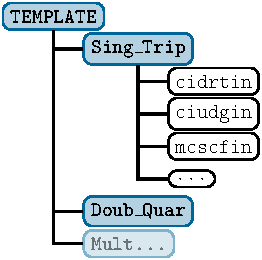
\includegraphics[scale=1]{img/dirs_COLtemp/dirs_COLtemp.pdf}
  \caption{Example directory structure of the \textsc{Columbus} template directory}
  \label{fig:dirs_COLtemp}
\end{figure}






% ========================================================================================================= %

\section{Analytical PESs Interface}\label{sec:int:analytical}

The \sharc\ suite also contains an interface which allows to run dynamics simulations on PESs expressed with analytical functions for diabatic states.
In order to allow dynamics simulations including IC and ISC, the interface allows to enter two kinds of potential couplings: one which is diagonalized away already in the interface (the equivalent of diagonalizing the CI matrix in the quantum chemistry program), and another kind which is left to \sharc\ for diagonalization (as the SOCs are).

The interface needs one additional input file, called \ttt{SH2Ana.inp}, which contains the definitions of all analytical expressions.

\subsection{Parametrization}

The interface has to be provided with analytical expressions for all matrix elements of the following matrices in the diabatic basis:
\begin{itemize}
  \item Hamiltonian: $\mathbf{H}$
  \item Derivative of the Hamiltonian with respect to each atomic coordinate: $\mathbf{H}_{x_i}$
  \item (Transition) dipole matrices for each polarization direction: $\mathbf{M}_i$
  \item Real and imaginary part of the SOC matrix: $\boldsymbol{\Sigma}$
  \item (Optionally) the derivatives of the transition dipole matrices: $\mathbf{D}_{i,x_j}$
\end{itemize}

Then the following calculations lead to the MCH matrices which are passed to \sharc:
%%tth: \begin{equation}
%%tth:   \mathbf{H}^{\text{d}}=\mathbf{U}^\dagger\mathbf{H}\mathbf{U}
%%tth: \end{equation}
%%tth: \begin{equation}
%%tth:   \mathbf{H}^{\text{MCH}}=\mathbf{H}^{\text{d}}+\mathbf{U}^\dagger\boldsymbol{\Sigma}\mathbf{U}
%%tth: \end{equation}
%%tth: \begin{equation}
%%tth:   \left(\mathbf{g}^{\text{MCH}}_\alpha\right)_{x_i}=\left(\mathbf{U}^\dagger\mathbf{H}_{x_i}\mathbf{U}\right)_{\alpha\alpha}
%%tth: \end{equation}
%%tth: \begin{equation}
%%tth:   \mathbf{M}^{\text{MCH}}_i=\mathbf{U}^\dagger\mathbf{M}_i\mathbf{U}
%%tth: \end{equation}
%%tth: \begin{equation}
%%tth:   \mathbf{S}^{\text{MCH}}(t_0,t)=\mathbf{U}^\dagger(t_0)\mathbf{U}(t)
%%tth: \end{equation}
%%tth: \begin{equation}
%%tth:   \mathbf{D}^{\text{MCH}}_{i,x_j}=\mathbf{U}^\dagger\mathbf{D}_{i,x_j}\mathbf{U}
%%tth: \end{equation}
\tthdump{
  \begin{align}
    \mathbf{H}^{\text{d}}&=\mathbf{U}^\dagger\mathbf{H}\mathbf{U}\\
    \mathbf{H}^{\text{MCH}}&=\mathbf{H}^{\text{d}}+\mathbf{U}^\dagger\boldsymbol{\Sigma}\mathbf{U}\\
    \left(\mathbf{g}^{\text{MCH}}_\alpha\right)_{x_i}&=\left(\mathbf{U}^\dagger\mathbf{H}_{x_i}\mathbf{U}\right)_{\alpha\alpha}\\
    \mathbf{M}^{\text{MCH}}_i&=\mathbf{U}^\dagger\mathbf{M}_i\mathbf{U}\\
    \mathbf{S}^{\text{MCH}}(t_0,t)&=\mathbf{U}^\dagger(t_0)\mathbf{U}(t)\\
    \mathbf{D}^{\text{MCH}}_{i,x_j}&=\mathbf{U}^\dagger\mathbf{D}_{i,x_j}\mathbf{U}
  \end{align}
}
The MCH Hamiltonian is the diagonalized diabatic Hamiltonian plus the SO matrix transformed into the MCH basis. The gradients in the MCH basis are obtained by transforming the derivative matrices into the MCH basis. The dipole matrices are also simply transformed into the MCH basis. The overlap matrix is the overlap of old and new transformation matrix.

\subsection{Interface-specific input file}

The interface-specific input file is called \ttt{SH2Ana.inp}. It contains the analytical expressions for all matrix elements mentioned above. All analytical expressions in this file are evaluated considering the atomic coordinates read from \ttt{QM.in}.

The file consists of a file header and the file body. The file body consists of variable definition blocks and matrix blocks.

\paragraph{Header} 

The header looks similar to an xyz file:
\begin{example}
  \begin{verbatim}
2
2
I       xI       0       0
Br      xBr      0       0
  \end{verbatim}
\end{example}
Here, the first line gives the number of atoms and the second line the number of states. The remaining lines tell the interface which variable name it should associate with which atomic coordinate. In the above example, the variable name \ttt{xI} is associated with the $x$ coordinate of the first atom given in \ttt{QM.in}. The variable name \ttt{xI} can then be used in the expressions in the file body. 

All variable names must be \href{https://docs.python.org/2/reference/lexical_analysis.html#identifiers}{valid Python identifiers} and must not start with an underscore. Hence, all strings starting with a letter, followed by an arbitrary number of letters, digits and underscores, are valid. It is not allowed to use a variable name twice.

If a zero (\ttt{0}) is given instead of a variable name, then this coordinate will be ignored (even if the coordinate is actually not zero in \ttt{QM.in}). 

Note that the file header also contains the atom labels, which are just used for cross-checking against the atom labels in \ttt{QM.in}.

The file header must not contain comments, neither at the end of a line nor separate lines. Also, blank lines are not allowed in the header. After the last line of the header (where the variables for the $n_{\text{atom}}$-th atom are defined), blank lines and comments can be used freely (except in matrix blocks).

\paragraph{Variable definition blocks}

Variable definition blocks can be used to store additional numerical values (beyond the atomic coordinates) in variables, which can then be used in the equations in the matrix blocks. The most obvious use for this is of course to define values which will appear several times in the equations.

A variable definition block looks like:
\begin{example}
  \begin{verbatim}
Variables
A1      0.067
g1      0.996   # Trailing comment
# Blank line with comment only
R1      4.666
End
  \end{verbatim}
\end{example}
Each block starts with the keyword ``Variables'' and is terminated with ``End''. Inbetween, on each line a variable name and the corresponding numerical value (separated by blanks) can be given. Note that the naming conventions given above also apply to variables defined in these blocks. 

There can be any number of complete variable definitions blocks in the input file. All blocks are read first, before any matrix expressions are evaluated. Hence, the relative order of the variable blocks and the matrix blocks does not matter. Also, note that variable names must not appear twice, so variables cannot be redefined halfway through the file.

\paragraph{Matrix blocks}

The most important information in the input file are of course contained in the expressions in the matrix blocks. In general, a matrix block has the following format:
\begin{example}
  \begin{verbatim}
Matrix_Identifier
V11
V12,    V22
V13,    V23,    V33
...
  \end{verbatim}
\end{example}
The first line identifies the type of matrix. Those are valid identifiers:
\begin{itemize}
  \item \ttt{Hamiltonian}: Defines the Hamiltonian including the diabatic potential couplings.
  \item \ttt{Derivatives} followed by a variable name (only variables from the header): Derivative of the Hamiltonian with respect to the given variable.
  \item \ttt{Dipole} followed by 1, 2 or 3: (Transition) dipole moment matrix for cartesian direction $x$, $y$ or $z$, respectively.
  \item \ttt{Dipolederivatives} followed by 1, 2 or 3, followed by a variable name (only variables from the header): Derivative of the respective dipole moment matrix.
  \item \ttt{SpinOrbit} followed by \ttt{R} or \ttt{I}: Real or Imaginary (respectively) part of the spin-orbit coupling matrix $\boldsymbol{\Sigma}$.
\end{itemize}
Since the interface searches the file for these identifiers starting from the top until it is found, for each matrix only the first block takes effect. Note that the Hamiltonian and all relevant derivatives must be present. If dipole matrix, dipole derivative matrix or SO matrix definitions are missing, they will be assumed zero.

In the lines after the identifier, the expressions for each matrix element are given. Note the lower triangular format (all matrices are assumed symmetric, except the imaginary part of the SO matrix, which is assumed antisymmetric). Matrix elements must be separated by commas (so that whitespace can be used inside the expressions). There must be at least as many lines as the number of states (additional lines are neglected). If any line or matrix element is missing, the interface will abort.

An examplary block looks like:
\begin{example}
  \begin{verbatim}
Hamiltonian
A1*( (1.-math.exp(g1*(R1-xI+xBr)))**2-1.),
0.0006,                                         3e-5*(xI-xBr)**2
  \end{verbatim}
\end{example}
It is important to understand that the expressions are directly evaluated by the Python interpreter, hence all expressions must be valid Python expressions which evaluate to numeric (integer or float) values. Only the variables defined above can be used. 

Note that exponentiation in Python is \ttt{**}. In order to provide most usual mathematical functions, the \href{https://docs.python.org/2/library/math.html}{\ttt{math} module} is available. Among others, the \ttt{math} module provides the following functions:
\begin{itemize}
  \item \ttt{math.exp(x)}: Exponential function
  \item \ttt{math.log(x)}: Natural logarithm
  \item \ttt{math.pow(x,y)}: $x^y$
  \item \ttt{math.sqrt(x)}: $\sqrt{x}$
  \item \ttt{math.cos(x)}, \ttt{math.sin(x)}, \ttt{math.tan(x)}
  \item \ttt{math.acos(x)}, \ttt{math.asin(x)}, \ttt{math.atan(x)}
  \item \ttt{math.atan2(y,x)}: $\tan^{-1}\left(\frac{y}{x}\right)$, as in many programming languages (takes care of phases)
  \item \ttt{math.pi}, \ttt{math.e}: $\pi$ and Euler's number
  \item \ttt{math.cosh(x)}, \ttt{math.sinh(x)}: Hyperbolic functions (also tanh, acosh, asinh, atanh are available)
\end{itemize}



% ========================================================================================================= %
% ========================================================================================================= %
% ========================================================================================================= %

\chapter{Auxilliary Scripts}\label{chap:aux}

In this chapter, all auxilliary scripts and programs are documented. Input generators (\ttt{molpro\_input.py} and \ttt{molcas\_input.py}) are documented in the relevant interface sections.

All auxilliary scripts are either interactive---prompting user input from stdin in order to setup a certain task---or non-interactive, meaning they are controlled by command-line arguments and options, in the same way as many command-line tools work.

All interactive scripts sequentially ask a number of questions to the user. In many cases, a default value is presented, which is either preset or detected by the scripts based on the availability of certain files. Furthermore, the scripts feature auto-completion (use TAB). All interactive scripts write a file called \ttt{KEYSTROKES.<script\_name>} which contains the user input from the last completed session. These files can be piped to the scripts to perform the same task again, for example:
\begin{verbatim}
user@host> cat KEYSTROKES.excite - | $SHARC/excite.py
\end{verbatim}
Note the \ttt{-}, which tells \ttt{cat} to switch to stdin after the file ends, so that the user can proceed if the script asks for more input than contained in the \ttt{KEYSTROKES} file.

All non-interactive scripts can be called with the \ttt{-h} option to obtain a short description, usage information and a list of the command line options.

All scripts can be safely killed during a run by using \ttt{STRG+C}. In this case, usually a \ttt{KEYSTROKES.tmp} file remains, containing the user input made so far.

\section{Wigner Distribution Sampling: \ttt{wigner.py}}\label{sec:wigner.py}

The first step in preparing the dynamics calculation is to obtain a set of physically correct initial conditions. Each initial condition is a set of initial atomic coordinates, initial atomic velocities and initial electronic state. The initial geometry and velocities can be obtained in different ways. With \sharc, usually they are obtained from sampling a quantum-harmonic Wigner distribution. 

The sampling is carried out with the non-interactive Python script \ttt{wigner.py}. The theoretical background is summarized in section~\ref{met:wigner}.

\subsection{Usage}

The general usage is 
\begin{verbatim}
user@host> python $SHARC/wigner.py [options] filename.molden
\end{verbatim}
\ttt{wigner.py} takes exactly one command-line argument, plus some options. Usually, the \ttt{-n} option is necessary, since by default only 3 initial conditions are sampled.

The argument is the filename of the file containing the information about the vibrational frequencies and normal modes. The file is by default assumed to be in the \href{http://www.cmbi.ru.nl/molden/molden_format.html}{\textsc{Molden} format}. For usage with \ttt{wigner.py}, only the following blocks have to be present:
\begin{itemize}
  \item $[$FREQ$]$
  \item $[$FR-COORD$]$
  \item $[$FR-NORM-COORD$]$
\end{itemize}
Alternatively, the information about the vibrational frequencies and normal modes can be read directly from a \textsc{Molpro} output file of a frequency calculation. In this case, in addition to the filename, also the switch \ttt{-M} has to be given. 
\begin{verbatim}
user@host> python $SHARC/wigner.py -M MOLPRO.out
\end{verbatim}

The script accepts a number of command-line options, which are given in table~\ref{tab:wigner_opts}.
\begin{table}
  \centering
  \caption{Command-line options for script \ttt{wigner.py}.}
  \label{tab:wigner_opts}
  \begin{tabular}{>{\tt}lll}
    \toprule
    \rmfamily Option        &Description      &Default\\
    \midrule
    -h                  &Display help message and quit.             &---                            \\
    -m                  &Modify atom masses                         &Most common isotope.           \\
    -M                  &Assume a \textsc{Molpro} input file.       &Assume a \textsc{Molden} file. \\
    -n  INTEGER         &Number of initial conditions to generate.  &3                              \\
    -o  FILENAME        &Output filename.                           &\ttt{initconds}                \\
    -r  INTEGER         &Seed for random number generator.          &16661                          \\
    -s  FLOAT           &Scaling factor for the frequencies.        &1.0                            \\
    \bottomrule
  \end{tabular}
\end{table}

\subsection{Output}

The script \ttt{wigner.py} generates a single output file, by default called \ttt{initconds}. All information about the initial conditions is stored in this file. Later steps in the preparation of the initial conditions add information about the excited states to this file. The file is formatted in a human-readable form.

\subsection{Non-default Masses}

When the \ttt{-m} option is used, the script will ask the user to interactively modify the atom masses. For each atom (referred to by the atom index as in the \textsc{Molden} file), a mass can be given (relative atomic weights). Note that the frequency calculation which produces the \textsc{Molden} or \textsc{Molpro} file has to be done with the same atomic masses.

\subsection{Specification of the \ttt{initconds} file}

\todo{}

\section{Setup of Initial Conditions: \ttt{setup\_init.py}}\label{sec:setup_init.py}

In order to find the correct initial electronic state for a given initial geometry, an excited-state ab initio calculation is necessary. This calculation delivers excitation energies and oscillator strengths, which are necessary in order to decide whether an electronic state is acceptable as initial state.

The preparation of these ab initio calculations is carried out by \ttt{setup\_init.py}. This script is interactive.

\subsection{Usage}

The script is started by simply typing 
\begin{verbatim}
user@host> python $SHARC/setup_init.py
\end{verbatim}
Please be aware that the script will setup the calculations in the directory where it was started.

\subsection{Input}

In the following, all input sections are documented:

\paragraph{Initial Conditions File}

Enter the filename of the initial conditions file, which was generated beforehand with \ttt{wigner.py}. If the script finds a file called \ttt{initconds}, the user is asked whether to use this file. The script detects the number of initial conditions and number of atoms automatically from the initial conditions file.

\paragraph{Range of Initial Conditions}

The initial conditions in \ttt{initconds} are indexed, starting with the index 1. In order to prepare ab initio calculations for a subset of all initial conditions, enter a range of indices, e.g.\ $a$ and $b$. This will prepare all initial conditions with indices in the interval $[a,b]$. In any case, the script will additionally prepare a calculation for the equilibrium geometry (except if a finished calculation for the equilibrium geometry has already been performed).

\paragraph{Number of states}

Here the user can specify the number of excited states to be calculated. Note that the ground state has to be counted as well, e.g.\ if 4 singlet states are specified, the calculation will involve the $S_0$, $S_1$, $S_2$ and $S_3$. Also states of higher multiplicity can be given, e.g.\ triplet or quintett states. 
For even-electron molecules, including odd-electron states (e.g.\ doublets) is only useful if transition properties for ionization can be computed (e.g.\ Dyson norms with the \textsc{Columbus} interface). These transition properties can be used to calculate ionization spectra or to obtain initial conditions for dynamics of anions.

\paragraph{Spin-orbit calculation}

Usually it is sufficient to calculate the spin-free excitation energies and oscillator strengths in order to decide for the initial state. However, using this option, the effects of spin-orbit coupling on the excitation energies and oscillator strengths can be included. Note that the script will never calculate spin-orbit couplings if only singlet states are included in the calculation.

\paragraph{Interface}

In this point, choose any of the displayed interfaces to carry out the ab initio calculations. Enter the corresponding number. 

The following input section depends on the chosen interface.

\subsection{Input for \textsc{Molpro}}

\paragraph{Path to \textsc{Molpro}}

The script will first look for a shell variable \ttt{\$MOLPRO}. The user can either confirm that \ttt{\$MOLPRO/molpro} or \ttt{\$MOLPRO} is the correct executable, or enter the path and filename of the correct executable. Note that the script will not expand the user (\ttt{\textasciitilde}) and shell variables (since possibly the ab initio calculations are running on a different machine than the one used for setup).

\paragraph{Scratch directory}

The script takes the string without any checking. Each individual initial condition uses a subdirectory called \ttt{ICOND\_0XXXX} with the appropriate number. 

\paragraph{Template file}

Enter the filename for the \textsc{Molpro} template input. This file contains the details of the ab initio calculation, like basis set, active orbitals and electrons, number of electrons and number of states for state-averaging. For \textsc{Molpro}, it also contains the memory usage. For details, see the section about the \sharc-\textsc{Molpro} interface (\ref{sec:int:molpro}). The setup script will check whether the template file contains the necessary entries. 

\paragraph{Initial wavefunction file}

You can provide an initial wavefunction (with an appropriate MO guess) to \textsc{Molpro}. This usually provides a drastic speedup for the CASSCF calculations and helps in ensuring that all calculations are based on the same active space. In easy cases it might be acceptable to not provide an initial wavefunction.

\subsection{Input for \textsc{Columbus}}

\paragraph{Path to \textsc{Columbus}}

The script first will look for a shell variable \ttt{\$COLUMBUS}. The user can either confirm that the path is correct, or enter another path. Note that the script will not expand the user (\ttt{\textasciitilde}) and shell variables (since possibly the ab initio calculations are running on a different machine than the one used for setup).

\paragraph{Scratch directory}

The script takes the string without any checking. Each individual initial condition uses a subdirectory called \ttt{ICOND\_0XXXX} with the appropriate number. 

\paragraph{Template directory}

Enter the path to a directory containing subdirectories with \textsc{Columbus} input files necessary for the calculations. See the section on the \sharc-\textsc{Columbus} interface (\ref{sec:int:columbus}) for further details. The script will auto-detect (based on the \ttt{cidrtin} files) which subdirectory contains the input for each multiplicity. The user has to check in the following dialog whether the association of multiplicities with job directories is correct. Additionally, the association of MO coefficient files to the jobs has to be checked.

Note that the setup script does not check any content of the input files beyond the multiplicity. Note that \ttt{transmomin} and \ttt{control.run} do not need to be present, since these files are written on-the-fly by the interface. 

\paragraph{Initial orbital coefficient file}

You can provide initial MO coefficients for the \textsc{Columbus} calculation. This usually provides a drastic speedup for the CASSCF calculations and helps in ensuring that all calculations are based on the same active space. In easy cases it might be acceptable to not provide an initial wavefunction.

\paragraph{Memory}

For \textsc{Columbus}, the available memory must be given here. 

\subsection{Input for Run Scripts}

\paragraph{Run script mode}

The script \ttt{setup\_init.py} generates a run script (Bash) for each initial condition calculation. There are two options how to perform the calculations. With the first option, the ab initio calculations are performed in the same directory in which it is setup (the directory, where \ttt{setup\_init.py} was started). Note that the interfaces will still use their scratch directories to perform the actual quantum chemistry calculations.

With the second option, the input files for each ab initio calculation are transferred to a temporary directory, where the interface is started. After the interface finishes all calculations, the results files are transferred back to the primary directory and the temporary directory is deleted. Note that \ttt{setup\_init.py} in any case creates the directory structure in the directory where it was started.

\paragraph{Submission script}

The setup script can also create a Bash script for the submission of all ab initio calculations to a queueing system. The user has to provide a submission command for that, including any options which might be necessary.

\paragraph{Project name}

The user can enter a project name. This is used currently only for the job names of submitted jobs (\ttt{-N} option for queueing system).

\subsection{Output}

\ttt{setup\_init.py} will create for each initial condition in the given range a directory, named \ttt{ICOND\_\%05i}, where \ttt{\%05i} is the index of the initial condition padded with zeroes to 5 digits. Additionally, the directory \ttt{ICOND\_00000} is created for the calculation of the excitation energies at the equilibrium geometry.

To each directory, the following files will be added:
\begin{itemize}
  \item \ttt{QM.in}: Main input file for the interface, contains the geometry and the control keywords (to specify which quantities need to be calculated). 
  \item \ttt{run.sh}: Run script, which can be started interactively or sent to the queue in order to perform the ab initio calculation in this directory.
  \item Interface-specific files: Usually a template file, a file containing additional input for the interface, and an initial wavefunction.
\end{itemize}

The calculations in each directory can be simply executed by starting \ttt{run.sh} in each directory. In order to perform this task consecutively on a single machine, the script \ttt{all\_run.sh} can be executed. The file \ttt{DONE} contains the progress of this calculation.

Alternatively, each run script can be sent to a queueing system. If all run scripts should be submitted, \ttt{all\_qsub.sh} can be run. After all calculations are finished, \ttt{excite.py} can be used to collect the results.

In figure~\ref{fig:dirs_init}, the directory tree structure setup by \ttt{setup\_init.py} is given.

\begin{figure}
  \centering
  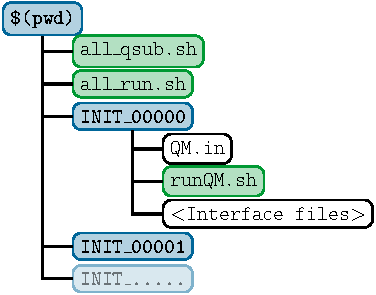
\includegraphics[scale=1]{img/dirs_init/dirs_init.pdf}
  \caption{Directory structure created by \ttt{setup\_init.py}. Directories are in blue, executable scripts in green and regular files in black and white. Interface files usually include initial MO coefficients, template files and interface input files.}
  \label{fig:dirs_init}
\end{figure}




\section{Excitation Selection: \ttt{excite.py}}\label{sec:excite.py}

\ttt{excite.py} collects the results of the ab initio calculations for the initial conditions. It calculates excitation energies, oscillator strengths and the probabilities which decide whether a state is selected for the dynamics. The script also carries out the stochastic excited-state selection (see~\ref{met:selection} for the theoretical background) and writes an initial condition file containing the excited-state information (see~\ref{sec:initcondsfile}). The script is interactive.

\ttt{excite.py} can also reread excited-state information from an initial condition file and redo the selection process, without reading the ab initio results.

\subsection{Input}

\paragraph{Initial condition file}

Enter the path to the initial conditions file. As the ab initio calculations do not contain all information previously generated by \ttt{wigner.py} (e.g.\ the atomic masses), the initial conditions file has to be provided in addition to the ab initio results. In effect, \ttt{excite.py} adds excited-state information to an existing initial conditions file.

\paragraph{Ab initio calculations}

If the initial conditions file does not contain excited-state information, those will be read from the \ttt{QM.out} files of all the excited-state ab initio calculations. If the initial conditions file already contains the information, the user can still read infos from the \ttt{QM.out} files.

\paragraph{Initial state selection}

\ttt{excite.py} performs two tasks, read-out of the ab initio calculations and the selection of the initial states for the dynamics. If only the read-out is necessary (e.g., in order to generate an absorption spectrum), the selection can be skipped.

\paragraph{Ground state as initial state}

If the user wants to perform ground state dynamics (or the excitation process is simulated with an actual laser field), then the ground state needs to be selected as a valid initial state. In this case, the ground state of \textit{all} initial conditions is selected.

\paragraph{Excitation window}

In the procedure of selecting initial excited states, only excited states within this energy range are considered (The interval borders are also included). The brightest state in the excitation window is used to normalize the excitation probabilities. For details on the selection procedure, see section~\ref{met:exc_selection}. 

\paragraph{Considered states}

The script also allows to exclude certain states completely from the initial excited-state selection procedure. The numbering scheme follows the canonical order, given in section~\ref{met:ordering}. The excluded states are also not considered for the normalization of the excitation probabilities (this allows to excite, e.g., to a dark $n\pi^*$ state next to a much brighter $\pi\pi^*$ state.

\paragraph{Random number generator seed}

The random number generator in \ttt{excite.py} is used in order to stochastically select initial excited states for dynamics. Instead of typing an integer, typing ``\ttt{!}'' will initialize the RNG from the system time. Note that this will not be reproducible, i.e.\ repeating the \ttt{excite.py} run with ``\ttt{!}'' as random seed will give a different selection.

\paragraph{Excited-state representation}

When reading from the \ttt{QM.out} files, the excited-state representation can be specified. The MCH representation is spin-free, meaning that transition dipole moments are only allowed between states of the same multiplicity. For molecules without heavy atoms, this option is sufficient. For heavier atoms, the diagonal representation can be used, which includes the effects of spin-orbit coupling on the excitation energies and oscillator strengths. 

Note that the representation can only be specified when reading from the \ttt{QM.out} files, since the initial condition file does not contain the spin-orbit Hamiltonian. If you intend to delete the directories containing the results of the ab initio calculations, you can run \ttt{excite.py} twice---once with MCH representation and once with diagonal representation---and save the results to two different files. Using these files, the initial state selection can be repeated.

\paragraph{Reference energy}

By default, the reference energy is obtained from \ttt{ICOND\_00000/QM.out} as the energy of the lowest singlet state (in MCH representation) or the lowest overall state (in diagonal representation). If \ttt{ICOND\_00000/QM.out} is not found, the user has to provide a reference energy (in hartree).

\subsection{Matrix diagonalization}

When using the diagonal representation, \ttt{excite.py} needs to diagonalize and multiply matrices. By default, the Python package Numpy is used, if available. If the script does not find a Numpy installation, it will use a small Fortran code which comes with the \sharc\ suite. In order for this to work, you need to set the environment variable \ttt{\$SHARC} to the \ttt{bin/} directory within your \sharc\ installation. 

\subsection{Output}

\ttt{excite.py} writes all output to a file \ttt{BASE.excited}, where \ttt{BASE} is the name of the initial conditions file used as input. The output file is also an initial conditions file, but contains additional information regarding the excited states, the reference energy and the representation of the excited states. An initial conditions file with excited-state information is needed for the final preparatory step: setting up the dynamics with \ttt{setup\_traj.py}.
Additionally, \ttt{spectrum.py} can calculate absorption spectra from excited-state initial condition files.

\subsection{Specification of the \ttt{initconds.excited} file format}\label{sec:initcondsfile}

The initial conditions files \ttt{initconds} and \ttt{initconds.excited} contain lists of initial conditions, which are needed for the setup of trajectories. An initial condition is a set of initial coordinates of all atoms and corresponding initial velocities of each atom, and optionally a list of excited state informations. In the following, the format of this file is specified.

The file contains of a header, followed by the body of the file containing a list of the initial conditions. 

\paragraph{File header}

An examplary header looks like:
\begin{example}
\footnotesize\begin{verbatim}
SHARC Initial conditions file, version 0.2   <Excited>
Ninit     100
Natom     2
Repr      MCH
Eref         -0.50
Eharm           0.04
States    2 0 1 

Equilibrium
 H   1.0  0.0  0.0  0.0   1.00782503   0.0  0.0  0.0
 H   1.0  1.5  0.0  0.0   1.00782503   0.0  0.0  0.0
\end{verbatim}
\end{example}
The first line must read \ttt{SHARC Initial conditions file, version <VERSION>}, with the correct version string followed. The string \ttt{Excited} is optional, and marks an initial conditions file as being an output file of \ttt{excite.py}. The following lines contain, in this order, the number of initial conditions, the number of atoms, the electronic state representation, the reference energy, the harmonic energy (zero point energy in the harmonic approximation), and optionally the number of states per multiplicity.

After the header, first the equilibrium geometry is expected. It is demarked with the keyword \ttt{Equilibrium}, followed by $n_\text{atom}$ lines, each specifying one atom.

\paragraph{File body}

The file body contains a list of initial conditions. Each initial condition is specified by a block starting with a line containing the string \ttt{Index} and the number of the initial condition. In the file, the initial conditions are expected to appear in order.

A block specifying an initial condition looks like:
\begin{example}
\footnotesize\begin{verbatim}
Index     1
Atoms
 H   1.0  -0.02  0.0  0.0   1.00782503  -0.001  0.0  0.0
 H   1.0   1.52  0.0  0.0   1.00782503   0.001  0.0  0.0
States
001    -0.49    -0.49  -0.16   0.0  -0.03   0.0   0.05   0.0   0.0   0.00 False
002    -0.25    -0.49   0.02   0.0   0.43   0.0  -1.77   0.0   6.5   0.53 True
003    -0.40    -0.49   0.00   0.0   0.00   0.0   0.00   0.0   2.5   0.00 False
004    -0.40    -0.49   0.00   0.0   0.00   0.0   0.00   0.0   2.5   0.00 False
005    -0.40    -0.49   0.00   0.0   0.00   0.0   0.00   0.0   2.5   0.00 False
Ekin        0.004 a.u.
Epot_harm   0.026 a.u.
Epot        0.013 a.u.
Etot_harm   0.030 a.u.
Etot        0.018 a.u.
\end{verbatim}
\end{example}
The formal structure of such a block is: After the line containing the keyword \ttt{Index}, the line \ttt{Atom} indicates the start of the list of atoms. Each atom is specified in one line (symbol, nuclear charge, $x$, $y$, $z$ coordinate in Bohrs, atomic mass, $x$, $y$ and $z$ component of nuclear velocity in atomic units). 

After the atom list, the keyword \ttt{States} indicates the list of electronic states. This list consists of one line per electronic state, but can be empty, if no information of the electronic states is available. Each line consists of: State number (starting with 1), energy in Hartree, reference energy in Hartree (usually the energy of the lowest state). The next six numbers define the transition dipole moment to the reference state (usually the lowest), in the order: real part of the $x$ component, imaginary part of the $x$ component, then the real and imaginary parts for the $y$ and finally the $z$ component (the transition dipole moments can be complex in the presence of spin-orbit couplings). After the transition dipole moments, the excitation energy in eV is given, then the oscillator strength, and finally a string which is either \ttt{True} or \ttt{False}, specifying whether the electronic state was selected by \ttt{excite.py} as initial electronic state. 

The electronic state list is terminated with the keyword \ttt{Ekin}, which at the same time gives the kinetic energy of all atoms. The remaining entries give the potential energy in the harmonic approximation and the actual potential energy, as well as the total energy.





\section{Setup of Trajectories: \ttt{setup\_traj.py}}\label{sec:setup_traj.py}

This interactive script prepares the input for the excited-state dynamics simulations with \sharc. It works similarly to \ttt{setup\_init.py}, reading an initial conditions file, asking a number of questions interactively to the user, and finally sets up one directory per trajectory. However, the \ttt{setup\_traj.py} input section is notably longer, because many options for the dynamics are covered.

\subsection{Input}

\paragraph{Initial conditions file}

Please be aware that \ttt{setup\_traj.py} needs an initial conditions file generated by \ttt{excite.py} (Files generated by \ttt{wigner.py} are not allowed). The script reads the number of initial states, the representation and the reference energy automatically from the file.

\paragraph{Number of states}

This is the total number of states per multiplicity included in the dynamics calculation. Affects the keyword \ttt{nstates} in the \sharc\ input file.

Only advanced users should use here a different number of states than given to \ttt{setup\_init.py}. In this case, the excited-state information in the initial conditions file might be inconsistent. For example, if 10 singlets and 10 triplets were included in the initial calculations, but only 5 singlets and 5 triplets in the dynamics, then the sixth entry in the initial conditions file corresponds to $S_5$, while \ttt{setup\_traj.py} assumes the sixth entry to correspond to $T_1$.

\paragraph{Active states}

Here, states can be frozen for the dynamics calculation. See section~\ref{met:activestates} for a general description of state freezing in \sharc. Only the highest states in each multiplicity can be frozen, it is not possible to, e.g., freeze the ground state in simulations where ground state relaxation is negligible. Affects the keyword \ttt{actstates}.

\paragraph{Contents of the initial conditions file}

Optionally, a map of the contents of the initial conditions file can be displayed during the execution of \ttt{setup\_traj.py}, showing for each state which initial conditions were selected (and which initial conditions do not have the necessary excited-state information). For each state, a table is given, where each symbol represents one initial condition. A dot ``\ttt{.}'' represents an initial condition where information about the current excited state is available, but which is not selected for dynamics. A hash mark ``\ttt{\#}'' represents an initial condition which is selected for dynamics. A question mark ``\ttt{?}'' represents initial conditions for which no information about the excited state is available (e.g.\ if the initial excited-state calculation crashed).

The content of the initial conditions file is also summarized in a table giving the number of initial conditions selected per state. 

\paragraph{Initial states for dynamics setup}

Here the user has to input all states from which trajectories should be launched. The numbers must be entered according to the above table giving the number of selected initial conditions per state. It is not allowed to specify inactive states as initial states. The script will give the number of trajectories which can be setup with the specified set of states. If no trajectories can be setup, the user has to specify again the set of possible initial states. The initial state will be written to the \sharc\ input, specified in the same representation as given in the initial conditions file. The initial coefficients will be determined automatically by \sharc, according to section~\ref{ssec:input:keywords}.

\paragraph{Starting index for dynamics setup}

Specifies the first initial condition within the initial condition file to be included in the setup. For example, the user might setup 50 trajectories starting with index 1. \ttt{setup\_traj.py} reports afterwards the last initial condition to be used for setup, e.g.\ index 90. Later, the user can setup additional trajectories, starting with index 91.

\paragraph{Random number generator seed}

The random number generator in \ttt{setup\_traj.py} is used to randomly generate RNG seeds for the \sharc\ input. Instead of typing an integer, typing ``\ttt{!}'' will initialize the RNG from the system time. Note that this will not be reproducible, i.e.\ repeating the \ttt{setup\_traj.py} run (with the same input) with ``\ttt{!}'' as random seed will give for the same trajectories different RNG seeds. Affects the keyword \ttt{RNGseed}.

\paragraph{Interface}

In this point, choose any of the displayed interfaces to carry out the ab initio calculations. Enter the corresponding number. The choice of the interface influences some dynamics options which can be set in the next section of the \ttt{setup\_traj.py} input.

\paragraph{Simulation Time}

This is the maximum time that \sharc\ will run the dynamics simulation. If trajectories need to be run for longer time, it is recommended to first let the simulation finish. Afterwards, increase the simulation time in the corresponding \sharc\ input file (keyword \ttt{tmax}) and add the restart keyword (also make sure that the \ttt{norestart} keyword is not present). Then the simulation can be restarted by running again the \ttt{run.sh} script. Affects the keyword \ttt{tmax}.

\paragraph{Simulation Timestep}

This gives the timestep for the dynamics. The on-the-fly ab initio calculations are performed with this timestep, as is the propagation of the nuclear coordinates. A shorter timestep gives more accurate results, especially if light atoms (hydrogen) are subjected to high kinetic energies or steep gradients. Of course a shorter timestep is computationally more expensive. A good compromise in many situations is 0.5~fs. Affects the keyword \ttt{stepsize}.

\paragraph{Number of substeps}

This gives the number of substeps for the interpolation of the Hamiltonian for the propagation of the electronic wavefunction. Usually, 25 substeps are sufficient. In cases where the diagonal elements of the Hamiltonian are very large (very large excitation energies or a badly chosen reference energy) more substeps are necessary. Affects the keyword \ttt{nsubsteps}.

\paragraph{Prematurely terminate trajectories}

Usually, trajectories which relaxed to the ground state do not recross to an excited state, but vibrate indefinitely in the ground state. Since one is rarely interested in these vibrations, such trajectories can be terminated prematurely in order to save computational ressources. In order to safely detect ground state relaxation, one should wait for 10--20~fs before terminating. Affects the keyword \ttt{killafter}.

\paragraph{Representation for the dynamics}

Either the diagonal representation can be chosen (by typing ``\ttt{yes}'') to perform dynamics with the \sharc\ methodology, or the dynamics can be performed on the MCH states, which would result in spin-diabatic dynamics. Affects the keyword \ttt{surf}.

\paragraph{Non-adiabatic couplings}

Electronic propagation can be performed with temporal derivatives, non-adiabatic coupling vectors or overlap matrices (Local diabatization). Enter the corresponding number. Note that depending on the chosen interface, some options might not be available, as displayed by \ttt{setup\_traj.py}. Affects the keyword \ttt{coupling}.

\paragraph{Gradient transformation}

The non-adiabatic coupling vectors can be used to correctly transform the gradients to the diagonal representation. If the dynamics uses the MCH representation, this question is not asked. If non-adiabatic coupling vectors are used anyways, this option is strongly recommended, since it gives more accurate gradients for no additional cost. Affects the keyword \ttt{gradcorrect}.

\paragraph{Surface hop treatment}

This option determines how the total energy is conserved after a surface hop. Affects the keyword \ttt{ekincorrect}.

\paragraph{Decoherence}

For most applications, decoherence should be enabled. Affects the keyword \ttt{decoherence}. Note that \ttt{setup\_traj.py} does not allow to modify the $\alpha$ value. In order to change the keyword \ttt{decoherence\_param}, the user has to manually edit the \sharc\ input files.

\paragraph{Scaling and Damping}

The keywords \ttt{scaling} and \ttt{damping} can be set here.

\paragraph{Gradient and non-adiabatic coupling selection}

The keywords \ttt{grad\_select} and \ttt{nac\_select} can be set here. For dynamics in the MCH representation, selection of gradients is not necessary, since always only one gradient is calculated. Selection for non-adiabatic couplings is only relevant, if they are used for propagation, gradient correction or rescaling of the velocities after a surface hop. For the selection threshold usually 0.5~eV are sufficient, except if spin-orbit coupling is very strong and hence the gradients mix strongly.

\subsection{Interface-specific input}

This input section is basically the same as for \ttt{setup\_init.py}. Note that for the dynamics simulations an initial wavefunction file is even more strongly recommended than for the initial calculations.

For MRCI dynamics using the \textsc{Columbus} interface, it is strongly advisory to obtain the \ttt{excitlistfiles} before starting the dynamics. 

\subsection{Run script setup}

Also this input section is similar to the one in \ttt{setup\_init.py}.

\subsection{Output}

\begin{figure}
  \centering
  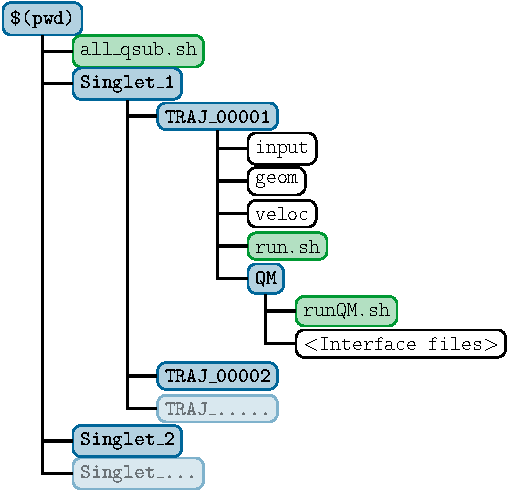
\includegraphics[scale=1]{img/dirs_traj/dirs_traj.pdf}
  \caption{Directory structure created by \ttt{setup\_traj.py}. Directories are in blue, executable scripts in green and regular files in black and white. Interface files usually include initial MO coefficients, template files and interface input files.}
  \label{fig:dirs_traj}
\end{figure}

\ttt{setup\_traj.py} will create for each initial state a directory, where all trajectories starting in this state will be put. If the initial conditions file specified that the initial conditions are in the MCH representation, then the initial states will be assumed to be in the MCH representation as well. In this case, the directories will be named \ttt{Singlet\_0}, \ttt{Singlet\_1}, ..., \ttt{Doublet\_0}, \ttt{Triplet\_1}, ... If the initial states are in the diagonal representation, then the directories are simply called \ttt{X\_1}, ... since they do not have a definite spin.

In each directory, subdirectories called \ttt{TRAJ\_\%05i} are created, where \ttt{\%05i} is the initial condition index, padded to 5 digits with zeroes. In each trajectory directory, an \sharc\ input file called \ttt{input} will be created, which contains all the dynamics options chosen during the \ttt{setup\_traj.py} run. Also, files \ttt{geom} and \ttt{veloc} will be created. For trajectories setup with \ttt{setup\_traj.py}, the determination of the initial wavefunction coefficients is done by \sharc.
For each trajectory, a \ttt{run.sh} script will be created, which can be executed to run the dynamics simulation. 
Furthermore, in each trajectory directory a subdirectory \ttt{QM} is created, where the \ttt{runQM.sh} script containing the call to the interface is put. In the directory \ttt{QM} also all interface-specific input files will be copied.

Optionally, \ttt{setup\_traj.py} also creates a script \ttt{all\_qsub.sh}, which can be executed to submit all trajectories to a queueing system.

The full directory structure created by \ttt{setup\_traj.py} is given in figure~\ref{fig:dirs_traj}.



\section{Laser field generation: \ttt{laser.x}}\label{sec:laser.x}

The Fortran code \ttt{laser.x} can generate files containing laser fields which can be used with \sharc. It is possible to superimpose several lasers, use different polarizations and apply a number of chirp parameters.

\subsection{Usage}

The program is simply called by 
\begin{verbatim}
user@host> python $SHARC/laser.x
\end{verbatim}
It will interactively ask for the laser parameters. After input is complete, it writes the laser field to the file \ttt{laser} in the format which \sharc\ expects (see~\ref{sec:laserfile}).

Similar to the interactive Python scripts, \ttt{laser.x} will also write the user input to \ttt{KEYSTROKES.laser}. After modifying this file, it can be used to directly execute \ttt{laser.x} without doing the interactive input again:
\begin{verbatim}
user@host> python $SHARC/laser.x < KEYSTROKES.laser
\end{verbatim}

\subsection{Input}

The first four options need to be entered only once, all remaining input options need to be present for every laser pulse. For the definition of laser field see section~\ref{sec:laser.x}.

\paragraph{Number of lasers}

Any number of lasers can be used. The output file will contain the sum of all laser pulses defined.

\paragraph{Real-valued field}

If this is true, the output file will only contain the real parts of the laser field, while the columns defining the imaginary part of the field will be zero. Note, however, that \sharc\ will anyways only use the real part of the field in the simulations.

\paragraph{Time interval and steps}

The definitions of the starting time, end time and time step of the laser field must exactly match the simulation time and time substeps of the \sharc\ simulation. Note that the laser field must always start at $t$=0 fs to be used with \sharc. The end time for the laser field must therefore coincide with the total simulation time given in the \sharc\ input. The number of time steps for the laser field is $t_\text{total}/\Delta t_\text{sub} +1$.

\paragraph{Files for debugging}

This option is normally not needed, and can be set to False.

\paragraph{Polarization vector}

The polarization vector $\vec{p}$ will be normalized.

\paragraph{Type of envelope}

There are two options possible for the envelope function $E(t)$, either a Gaussian envelope or a sinusoidal one (see~\ref{sec:laser.x}).

\paragraph{Field strength}

There are two input lines for the field strength $E_0$, the first defining the unit in which the field strength is defined, the second gives the corresponding number. Field strength can be read in in GV/m, TW/cm$^{-2}$ or atomic units.

\paragraph{FWHM and time intervals}

This option depends on the type of envelope chosen. While in both cases all 5 numbers need to be entered, for a Gaussian pulse only the first and third number have an effect. For a sinusoidal pulse only the first number has no effect.

For a Gaussian pulse, the first argument corresponds to FWHM in equation~\eqref{eq:laser_gauss_2} and the third argument to $t_c$ in ~\eqref{eq:laser_gauss_1}.

For a sinusoidal pulse ,the second, third, fourth and fifth argument correspond to $t_0$, $t_c$, $t_{c2}$ and $t_e$, respectively, in equation~\eqref{eq:laser_sinus}.

\paragraph{Central frequency}

There are two input lines for the central frequency $\omega_0$. The first defines the unit (wavelength in nm, energy in eV, or atomic units). The second line gives the value.

\paragraph{Phase}

The total phase $\phi$ is given in multiples of $\pi$, so that the input \ttt{1.5} gives a phase of $\frac{3\pi}{2}$.

\paragraph{Chirp parameters}

There are four lines giving the chirp parameters $b_1$, $b_2$, $b_3$ and $b_4$. See equation~\eqref{eq:laser_chirp} for the meaning of these parameters.




\section{File transfer: \ttt{retrieve}}\label{sec:retrieve}

Usually, \sharc\ will run on some temporary storage device, not in the home directory, where the trajectories have been submitted from. The shell script \ttt{retrieve} is a simple \ttt{scp} wrapper, which can be executed (in a directory where a trajectory has been sent from) in order to retrieve the output files of this trajectory.

It relies on the presence of the file \ttt{host\_infos}. All trajectories set up with \ttt{setup\_traj.py} create this file after the trajectory has been started with \ttt{run.sh}. \ttt{retrieve} reads \ttt{host\_infos} to determine the hostname and working directory of the trajectory and then uses \ttt{scp} to retrieve the output and restart files.

The script can be called with the option ``\ttt{-lis}'' in order to only retrieve the \ttt{output.lis} file, but not the other output files.

If the script is called with the option ``\ttt{-res}'' then also the restart files and the content of the restart directory are copied.

It is advisable to configure public-key authentification for the hosts running the trajectories, so that not for every execution of \ttt{retrieve} a password has to be entered.



\section{Calculation of Absorption Spectra: \ttt{spectrum.py}}\label{sec:spectrum.py}

Besides for setting up trajectories, the \ttt{initconds.excited} files can be used to generate absorption spectra based on the excitation energies and oscillator strengths in the file. The script \ttt{spectrum.py} calculates Gaussian or Lorentzian convolutions of these data in order to obtain spectra. See section~\ref{met:spectrum} for further details.

\ttt{spectrum.py} evaluates the absorption spectrum on a grid for all states it finds in an initial conditions file. Using command-line options, some initial conditions can be omitted in the convolution, see below.

\subsection{Input}

The script is executed with the initial conditions file as argument and with standard output (where the spectrum is written to) redirected to the desired output file:
\begin{verbatim}
user@host> python $SHARC/spectrum.py initconds.excited > spectrum.out
\end{verbatim}

The script accepts a number of command-line options, which are given in table~\ref{tab:spectrum_opts}.
\begin{table}
  \centering
  \caption{Command-line options for script \ttt{spectrum.py}.}
  \label{tab:spectrum_opts}
  \begin{tabular}{>{\tt}lll}
    \toprule
    \rmfamily Option        &Description      &Default\\
    \midrule
    -h                  &Display help message and quit.         &---       \\
    -o FILENAME         &Output filename (for the spectrum)     &\ttt{spectrum.out}\\
    -n INTEGER          &Number of grid points                  &500       \\
    -e FLOAT FLOAT      &Energy range (eV) for the spectrum     &1 to 10 eV\\
    -i INTEGER INTEGER  &Index range for the initial conditions &1 to 1000\\
    -f FLOAT            &FWHM (eV) for the spectrum             &0.1 eV\\
    -G                  &Gaussian convolution                   &Gaussian\\
    -L                  &Lorentzian convolution                 &Gaussian\\
    -s                  &Use only selected initial conditions   &Use all\\
    -l                  &Make a line spectrum                   &Convolution\\
    --gnuplot FILENAME  &Write a \textsc{Gnuplot} script        &No \textsc{Gnuplot} script\\
    \bottomrule
  \end{tabular}
\end{table}

\subsection{Output}

The script writes the absorption spectrum to a file (by default \ttt{spectrum.out}). Using the \ttt{-o} option, the user can redirect the output to a suitable file. The output is a table containing $n+2$ columns, where $n$ is the number of states found in the initial conditions file. The first column gives the energy in eV, which is within the given energy interval. In columns 2 to $n+1$ the state-wise absorption spectra are given. The last column contains the total absorption spectrum, the sum over all states. The table has $n_{\text{grid}}+1$ rows. For line spectra the output format is exactly the same, however, the file will contain one row for each excited state of each initial condition in the initial conditions file.

Additionally, the script writes some information about the calculation to standard error. Very helpful can be the reported maximum of the spectrum, which can be used in order to normalize the spectrum. The reported maximum is simply the largest value in the last column of the spectrum. 

If requested, the script generates a \textsc{Gnuplot} script, which can be used to directly plot the spectrum. 














\section{Internal Coordinates Analysis: \ttt{Geo.py}}\label{sec:Geo.py}

\sharc\ writes at every timestep the molecular geometry to the file \ttt{output.xyz}. The non-interactive script \ttt{Geo.py} can be used in order to extract internal coordinates from the xyz files. The usage is:
\begin{verbatim}
user@host> python $SHARC/Geo.py [options] < Geo.inp > Geo.out
\end{verbatim}
By default, the coordinates are read from \ttt{output.xyz}, but this can be changed with the \ttt{-g} option (see table~\ref{tab:Geo_options}). Note that the internal coordinate specifications are read from standard input and the result table is written to standard out. 

\subsection{Input}

The specifications for the desired internal coordinates are read from standard input. It follows a simple syntax, where each internal coordinate is specified by a single line of input. Each line starts with a one-letter key which specifies the type of internal coordinate (e.g.\ bond length, angle, dihedral, ...). The key is followed by a number of integers, specifying which atoms should be measured. As a simple example, \ttt{r 1 2} specifies the bond length (\ttt{r} is the key for bond lengths) between atoms 1 and 2. Note that the numbering starts with 1. Each line of input is checked for consistency (whether any atom index is larger than the number of atoms, repeated atom indices, misspelled keys, wrong number of atom indices, ...), and erroneous lines are ignored.

Table~\ref{tab:Geo_input} lists the available types of internal coordinates. The output is a table, where the first column is the time (Actually, the geometries are just enumerated starting with zero, and the number multiplied by the timestep from the \ttt{-t} option). The successive columns in the output table list the results of the internal coordinates calculations. Each request generates at least one column, see table~\ref{tab:Geo_input}. 

Note that for most internal coordinates, the order of the atoms is crucial, since e.g.\ $a_{123}\neq a_{213}$. This also holds for the Cremer-Pople parameter requests. For these input lines, the atoms should be listed in the order they appear in the ring (clockwise or counter-clockwise).

\begin{table}[h]
  \centering
  \caption{Possible types of internal coordinates in \ttt{Geo.py}. }
  \label{tab:Geo_input}
  \begin{tabular}{>{\tt}c>{\tt}lll}
    \toprule
    \rmfamily Key         &\rmfamily Atom      &Description    &Output columns\\
                          &\rmfamily Indices   &               &\\
    \midrule
    x   &a              &$x$ coordinate of atom \ttt{a}         &$x$\\
    y   &a              &$y$ coordinate of atom \ttt{a}         &$y$\\
    z   &a              &$z$ coordinate of atom \ttt{a}         &$z$\\
    r   &a b            &Bond length between \ttt{a} and \ttt{b}        &$r$\\
    a   &a b c          &Angle between \ttt{a}--\ttt{b} and \ttt{b}--\ttt{c}         &$a$\\
    d   &a b c d        &Dihedral (Angle between planes (\ttt{a,b,c})    &$d$\\
                       &&and (\ttt{b,c,d}))&\\
    p   &a b c d        &Pyramidalization angle (90$^\circ$ -- Angle between    &$p$\\
                       &&bond \ttt{a}--\ttt{b} and plane (\ttt{b,c,d}))&\\
    5   &a b c d e      &Cremer-Pople parameters for &$q_2$, $\phi_2$\\
                       &&5-membered rings&\\
    6   &a b c d e f    &Cremer-Pople parameters for &$Q$, $\phi$, $\theta$, Boeyens\\
                       &&6-membered rings and Boeyens classification&\\
    c   &               &Writes the comment (second line of the &Comment\\
                       &&xyz format) to the table.&\\
    \bottomrule
  \end{tabular}
\end{table}

As an advice, it is always a good idea to put the comment as the last request, if the comment needs to be included. Since the comment may contain blanks, having the comment not as the very last column might make it impossible to plot the resulting table.

The Boeyens classification symbols which are output for 6-membered rings are reported in \LaTeX\ math code. Note that in the Boeyens classification scheme a number of symbols are equivalent, and only one symbol is reported. For example, by definition the chair configuration $^1C_4$ is equivalent to $^5C_2$ and $^3C_6$.

\subsection{Options}

\ttt{Geo.py} accepts a number of command-line options, see table~\ref{tab:Geo_options}. All options have sensible defaults. However, especially if long comments should be written to the output file, it might be necessary to increase the field width. Note that the minimum column width is 20 so that the table header can be printed correctly.

\begin{table}[h]
  \centering
  \caption{Command-line options for \ttt{Geo.py}. }
  \label{tab:Geo_options}
  \begin{tabular}{>{\tt}lll}
    \toprule
    \rmfamily Option         &Description    &Default\\
    \midrule
    -h          &Display help message and quit.         &---       \\
    -b          &Report $x$, $y$, $z$, $r$, $q_2$ and $Q$ in Bohrs       &Angstrom\\
    -r          &Report $a$, $d$, $p$, $\phi_2$, $\phi$ and $\theta$ in Radians         &Degrees\\
    -g FILENAME &Read coordinates from the specified file       &\ttt{output.xyz}\\
    -t FLOAT    &Assumed timestep between successive geometries (fs)    &1.0 fs\\
    -p INTEGER  &Precision (Number of decimals, max.~width--3)         &4\\
    -f INTEGER  &Width of each column (min.~20)                   &20\\
    \bottomrule
  \end{tabular}
\end{table}








\section{Data Extractor: \ttt{data\_extractor.x}}\label{sec:data_extractor.x}

The output of \sharc\ is mainly written to \ttt{output.dat}. In order to obtain plottable files in tabular form, the Fortran program \ttt{data\_extractor.x} is used.

\subsection{Usage}

The \ttt{data\_extractor.x} is a command line tool, and is called with the \ttt{output.dat} file as an argument.
\begin{verbatim}
user@host> $SHARC/data_extractor.x output.dat
\end{verbatim}
The program will create a directory \ttt{output\_data} in the current working directory (not necessarily in the directory where \ttt{output.dat} resides). In this directory, several files are written, containing e.g.\ the potential energies depending on time, etc.

The program will extract the complete \ttt{output.dat} file until it reaches the EOF. No further input except for the data file can be given.

\subsection{Output}

After the program finishes, the directory \ttt{output\_data} contains a number of files. In each file, the number of columns is dependent in the total number $n$ of states $i\in\{1...n\}$. The content of the files is listed in Table~\ref{tab:outputdata}.

The file \ttt{expec.out} contains the information of \ttt{energy.out}, \ttt{spin.out} and \ttt{fosc.out} in one file. The content of \ttt{expec.out} can be conveniently plotted with a \textsc{Gnuplot} script generated by \ttt{make\_gnuscript.py}.

\begin{table}
  \centering
  \caption{Content of the files written by \ttt{data\_extractor.x}. $n$ is the total number of states, $i$ is a state index ($i\in\{1..n\}$).}
  \label{tab:outputdata}
  \begin{tabular}{>{\tt}lcll}
    \toprule
    File  &\# Columns     &\multicolumn{2}{l}{Columns}\\
    \midrule
    coeff\_diag.out       &$2+2n$
      &$1$ &Time $t$ (fs)\\
      &&$2$ &Norm of wavefunction $\sum_i |c_i^{\text{diag}}|^2$\\
      &&$1+2i$ &$\Re (c_i^{\text{diag}})$\\
      &&$2+2i$ &$\Im (c_i^{\text{diag}})$\\
    coeff\_MCH.out       &$2+2n$
      &$1$ &Time $t$ (fs)\\
      &&$2$ &Norm of wavefunction $\sum_i |c_i^{\text{MCH}}|^2$\\
      &&$1+2i$ &$\Re (c_i^{\text{MCH}})$\\
      &&$2+2i$ &$\Im (c_i^{\text{MCH}})$\\
    energy.out       &$4+n$
      &$1$ &Time $t$ (fs)\\
      &&$2$ &Kinetic energy (eV)\\
      &&$3$ &Potential energy (eV) of active state\\
      &&$4$ &Total energy (eV)\\
      &&$4+i$ &Potential energy (eV) of state $i$\\
    fosc.out       &$2+n$
      &$1$ &Time $t$ (fs)\\
      &&$2$ &Oscillator strength of active state\\
      &&$2+i$ &Oscillator strength of state $i$\\
    spin.out       &$2+n$
      &$1$ &Time $t$ (fs)\\
      &&$2$ &Total spin expectation value of active state\\
      &&$2+i$ &Total spin expectation value of state $i$\\
    prob.out       &$2+n$
      &$1$ &Time $t$ (fs)\\
      &&$2$ &Random number from surface hopping\\
      &&$2+i$ &Cumulated hopping probability $\sum_{j=1}^i P_j$\\
    expec.out      &$4+3n$
      &$1$ &Time $t$ (fs)\\
      &&$2$ &Kinetic energy (eV)\\
      &&$3$ &Potential energy (eV) of active state\\
      &&$4$ &Total energy (eV)\\
      &&$4+i$ &Potential energy (eV) of state $i$\\
      &&$4+n+i$ &Total spin expectation value of state $i$\\
      &&$4+2n+i$ &Oscillator strength of state $i$\\
    \bottomrule
  \end{tabular}
\end{table}

\section{Plotting the Extracted Data: \ttt{make\_gnuscript.py}}\label{sec:make_gnuscript.py}

The contents of the output files of \ttt{data\_extractor.x} can be plotted with \textsc{Gnuplot}. In order to quickly generate an appropriate \textsc{Gnuplot} script, \ttt{make\_gnuscript.py} can be used. The usage is:
\begin{verbatim}
user@host> python $SHARC/make_gnuscript.py <S> [<D> [<T> [<Q> ... ] ] ]
\end{verbatim}
\ttt{make\_gnuscript.py} takes between 1 and 8 integers as command-line arguments, specifying the number of singlet, doublet, triplet, etc.\ states. It writes an appropriate \textsc{Gnuplot} script to standard out, hence redirect the output to a file, e.g.:
\begin{verbatim}
user@host> python $SHARC/make_gnuscript.py 3 0 2 > gnuscript.gp
\end{verbatim}


Then, \textsc{Gnuplot} can be run in the \ttt{output\_data} directory of a trajectory:
\begin{verbatim}
user@host> gnuplot gnuscript.gp
\end{verbatim}
This can also be accomplished in one step using a pipe, e.g.:
\begin{verbatim}
user@host> python $SHARC/make_gnuscript.py 3 0 2 | gnuplot
\end{verbatim}

The created plot script generates four different plots (press ENTER in the command-line where you started \textsc{Gnuplot} to go to the next plot). The first plot shows the diagonal potential energy of all states in the dynamics over time. The currently occupied state is marked with black circles. A thin black line gives the total energy (sum of the kinetic energy and the potential energy of the currently occupied state). Each state is colored, with one color as contour and one color at the core of the line. The contour color represents the total spin expectation value of the state. The core color represents the oscillator strength of the state with the lowest state. See figure~\ref{fig:colors} for the relevant color code.
\begin{figure}
  \centering
  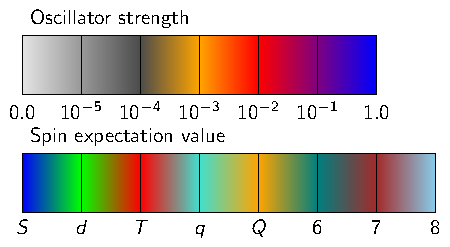
\includegraphics[scale=1]{img/colors/colors.pdf}
  \caption{Color code for plots generated with the use of \ttt{make\_gnuscript.py}.}
  \label{fig:colors}
\end{figure}
Note that by definition the ``oscillator strength'' of the lowest state with itself is exactly zero, hence the lowest state is also light grey. This dual coloring allows for a quick recognition of different types of states in the dynamics, e.g.\ singlets vs.\ triplets or $n\pi^*$ vs.\ $\pi\pi^*$ states.

The second plot shows the population $|c_i^{\text{MCH}}|^2$ of the MCH electronic states over time. The line colors are auto-generated in order to give a large spread of all colors over the excited states, but the colors might be sub-optimal, e.g.\ for printing. In this cases, the user should manually adjust the colors in the generated script.

The third plot shows the population $|c_i^{\text{diag}}|^2$ of the diagonal electronic states over time. These are the populations which are actually used for surface hopping. However, since these states are spin-mixed, it is usually difficult to interpret these populations.

The fourth plot shows the surface hopping probabilities over time. The plot is setup in such a way that the visible area corresponding to a certain state is proportional to the probability to hop into the state. Hence, if for a given timestep the random number (black circles) lies within a colored area, a surface hop to the corresponding state is performed.

\section{Calculation of Ensemble Populations: \ttt{populations.py}}\label{sec:populations.py}

For an ensemble of trajectories, usually one of the most relevant results are ensemble-averaged populations. The interactive script \ttt{populations.py} collects these populations from a set of trajectories. 

Different methods to obtain populations or quantities approximating populations can be collected, as described below.

\subsection{Usage}

The script is interactive, simply start it with no command-line arguments or options:
\begin{verbatim}
user@host> python $SHARC/populations.py
\end{verbatim}

Depending on the analysis mode (see below) it might be necessary to run \ttt{data\_extractor.x} for each trajectory prior to running \ttt{populations.py}. 

\paragraph{Paths to trajectories}

First the script asks the user to specify all directories for whose content the analysis should be performed. Enter one directory path at a time, and finish the directory input section by typing ``\ttt{end}''. Please do not specify each trajectory directory separately, but specify their parent directories, e.g.\ the directories \ttt{Singlet\_1} and \ttt{Singlet\_2}. \ttt{populations.py} will automatically include all trajectories contained in these directories.

If you want to exclude certain trajectories from the analysis, it is sufficient to create an empty file called \ttt{CRASHED} or \ttt{RUNNING} in the corresponding trajectory directory. \ttt{populations.py} will ignore all directories containing one of these files.

\paragraph{Analysis mode}

Using \ttt{populations.py}, there are two basic ways in obtaining the excited-state populations. The first way is to count the number of trajectories for which a certain condition holds. For example, the number of trajectories in each classical state can be obtained in this way. However, it is also possible to count the number of trajectories for which the total spin expectation value is within a certain interval. 
The second way to obtain populations is to obtain the sum of the absolute squares of the quantum amplitudes over all trajectories. Table~\ref{tab:Populations_modes} contains a list of all possible analysis modes.

\begin{table}
  \centering
  \caption{Analysis modes for \ttt{populations.py}. The last column indicates whether \ttt{data\_extractor.x} has to be run prior to the ensemble analysis.}
  \label{tab:Populations_modes}
  \begin{tabular}{lp{6cm}>{\tt}lc}
    \toprule
    Mode        &Description    &\rmfamily From which     &Extract?\\
                               &&\rmfamily file?          &\\
    \midrule
    1   &Counts how many trajectories are classically in each diagonal state. &output.lis  &No\\
    2   &Counts how many trajectories are classically in each MCH state. &output.lis  &No\\
    3   &Counts how many trajectories are classically in each MCH state. Multiplet components are summed up. &output.lis  &No\\
    4   &Counts how many trajectories have their total spin expectation value in certain intervals.   &output.lis &No\\
    5   &Counts how many trajectories have their permanent dipole moment expectation value in certain intervals.   &output.lis &No\\
    6   &Counts how many trajectories have their oscillator strength with the lowest state in certain intervals.        &output\_data/fosc.out  &Yes\\
    7   &Calculates the sum of the absolute squares of the diagonal coefficients.       &output\_data/coeff\_diag.out&Yes\\
    8   &Calculates the sum of the absolute squares of the MCH coefficients.       &output\_data/coeff\_MCH.out&Yes\\
    9   &Calculates the sum of the absolute squares of the MCH coefficients. Multiplet components are summed up.       &output\_data/coeff\_MCH.out&Yes\\
    \bottomrule
  \end{tabular}
\end{table}

\paragraph{Run data extractor}

For analysis modes 6, 7, 8 and 9 it is necessary to first run the data extractor (see section~\ref{sec:data_extractor.x}). This task can be accomplished by \ttt{populations.py}. However, for a large ensemble or for long trajectories this may take some time. Hence, it is not necessary to perform this step each time \ttt{populations.py} is run. 

\ttt{populations.py} will detect whether the file \ttt{output.dat} or the content of \ttt{output\_data/} is more recent. Only if \ttt{output.dat} is newer the \ttt{data\_extractor.x} will be run for this trajectory.

\paragraph{Number of states}

For analysis modes 1, 2, 3, 7, 8 and 9 it is necessary to specify the number of states in each multiplicity. The number is auto-detected from the input file of one of the trajectories.

\paragraph{Intervals}

For analysis modes 4, 5 and 6 the user must specify the intervals for the classification of the trajectories. The user has to input a list of interval borders, e.g.:
\begin{verbatim}
Please enter the interval limits, all on one line.
Interval limits: 1e-3 0.01 0.1 1
\end{verbatim}
Note that scientific notation can be used. Based on this input, for each timestep a histogram is created with the number of trajectories in each interval. The histogram bins are:

\begin{tabular}{ccccc}
  \toprule
  1&2&3&4&5\\
  \midrule
  $x\leq10^{-3}$     &$10^{-3}<x\leq10^{-2}$ &$10^{-2}<x\leq10^{-1}$ &$10^{-2}<x\leq10^{0}$ &$10^{0}<x$\\
  \bottomrule
\end{tabular}\\
Note that there is always one more bin that interval borders.

\paragraph{Normalization}

If desired, \ttt{populations.py} can normalize the populations by dividing the populations by the number of trajectories. 

\paragraph{Maximum simulation time}

This gives the maximum simulation time until which the populations are analyzed. For trajectories which are shorter than this value, the last population information is used to make the trajectory long enough. Trajectories which are longer are not analyzed to the end. \ttt{populations.py} prints the length of the shortest and longest trajectories after the analysis.

\paragraph{Gnuplot script}

\ttt{populations.py} can generate an appropriate \textsc{Gnuplot} script for the performed population analysis. 

\subsection{Output}

By default, \ttt{populations.py} writes the resulting populations to \ttt{pop.out}. If the file already exists, the user is ask whether it shall be overwritten, or to provide an alternative filename. Note that the output file is checked only after the analysis is completed, so the program might run for a considerable amount of time before asking for the output file.


\section{Obtaining special geometries: \ttt{crossing.py}}\label{sec:crossing.py}

In many cases, it is also important to obtain certain special geometries from the trajectories. The script \ttt{crossing.py} extracts geometries fulfilling special conditions from an ensemble of trajectories. Currently, \ttt{crossing.py} finds geometries where the approximate MCH state of the last timestep is different from the MCH state of the current timestep (i.e.\ \ttt{crossing.py} finds geometries where surface hops occured). 

\subsection{Usage}

The script is interactive, simply start it with no command-line arguments or options:
\begin{verbatim}
user@host> python $SHARC/crossing.py
\end{verbatim}

The input to the script is very similar to the one of \ttt{populations.py}. 

\paragraph{Paths to trajectories}

First the script asks the user to specify all directories for whose content the analysis should be performed. Enter one directory path at a time, and finish the directory input section by typing ``\ttt{end}''. Please do not specify each trajectory directory separately, but specify their parent directories, e.g.\ the directories \ttt{Singlet\_1} and \ttt{Singlet\_2}. \ttt{crossing.py} will automatically include all trajectories contained in these directories.

If you want to exclude certain trajectories from the analysis, it is sufficient to create an empty file called \ttt{CRASHED} or \ttt{RUNNING} in the corresponding trajectory directory. \ttt{crossing.py} will ignore all directories containing one of these files.

\paragraph{Analysis mode}

Currently, \ttt{crossing.py} only supports one analysis mode, where \ttt{crossing.py} is scanning for each trajectory the file \ttt{output.lis}. If the occupied MCH state (column 4 in output file \ttt{output.lis}) changes from one timestep to the next, it is checked whether the old and new MCH states are the ones specified by the user. If this is the case, the geometry corresponding to the new timestep ($t$) is retrieved from \ttt{output.xyz} (lines $t(n_{\text{atom}}+2)+1$ to $t(n_{\text{atom}}+2)+n_{\text{atom}}$). 

\paragraph{States involved in surface hop}

First, the user has to specify the permissible old MCH state. The state has to be specified with two integers, the first giving the multiplicity (\ttt{1}=singlet, ...), the second the state within the multiplicity (\ttt{1 1}=$S_0$, \ttt{1 2}=$S_1$, etc.). If a state of higher multiplicity is given, \ttt{crossing.py} will report all geometries where the old MCH state is any of the multiplet components. 

For the new MCH state, the same is valid.

Third, the direction of the surface hop has to be specified. Choosing ``Backwards'' has the same effect as exchanging the old and new MCH states. 

\subsection{Output}

All geometries are in the end written to an output file, by default \ttt{crossing.xyz}. The file is in standard xyz format. The comment of each geometry gives the path to the trajectory where this geometry was extracted, the simulation time and the diagonal and MCH states at this simulation time. 


\section{Diagonalization Helper: \ttt{diagonalizer.x}}\label{sec:diagonalizer.x}

The small program \ttt{diagonalizer.x} is used by the Python scripts to diagonalize matrices if the Numpy library is not available. Currently, only \ttt{excite.py} needs to diagonalize matrices (If the excitation energies and oscillator strengths are calculated in the diagonal representation). \ttt{diagonalizer.x} is implemented as a simple front-end to the LAPACK libary.

The program reads from stdin. The first line consists of the letter ``r'' or ``c'', followed by two integers giving the matrix dimensions. For ``r'', the program assumes a real symmetric matrix, for ``c'' a Hermitian matrix. The matrix must be square.
The second line is a comment and is ignored.
In the following lines, the matrix elements are given. On each line one row of the matrix has to be written. If the matrix is complex, each line contains the double number of entries, where real and imaginary part are always given subsequently.
The following is an example input:
\begin{example}
\footnotesize\begin{verbatim}
c 2 2
comment
1.0  0.0    2.0  0.1
2.0 -0.1    6.0  0.0
\end{verbatim}
\end{example}

\normalsize
for the matrix 
%%tth: \newline\includegraphics[scale=1]{equations/equation_65.gif}\newline
\tthdump{
  \begin{equation}
    A=\begin{pmatrix}
        1 &2+0.1i\\
        2-0.1i&6
      \end{pmatrix}.\nonumber
  \end{equation}
}
The diagonal matrix and the matrix of eigenvectors is written to stdout.



% ========================================================================================================= %
% ========================================================================================================= %
% ========================================================================================================= %

\chapter{Methodology}

In this chapter different aspects of \sharc\ simulations are discussed in detail. The topics are ordered alphabetically.


\section{Absorption Spectrum}\label{met:spectrum}

Using \ttt{spectrum.py}, an absorption spectrum can be calculated as the sum over the absorption spectra of each individual initial condition:
\begin{equation}
  \sigma(E)=\sum\limits_i^{n_\text{init}} \sigma_i(E),
\end{equation}
where $i$ runs over the initial conditions.

The spectrum of a single initial condition is the convolution of its line spectrum, defined through a set of tuples $(E^\alpha,f_\text{osc}^\alpha)$ for each electronic state $\alpha$, where $E^\alpha$ is the excitation energy and $f_\text{osc}^\alpha)$ is the oscillator strength.

The convolution of the line spectrum can be performed with \ttt{spectrum.py} using either Gaussian or Lorentzian functions. The contribution of a state $\alpha$ to the absorption spectrum $\sigma^\alpha(E)$ is given by:
%%tth: \begin{equation}
%%tth:   \sigma^\alpha_{\text{Gaussian}}(E)=\left(f_{\text{osc}}\right)_i^\alpha \E^{c\left(E-E_i^\alpha\right)^2},
%%tth: \end{equation}
%%tth: \begin{equation}
%%tth:   \text{with}\qquad c=-\frac{4\ln(2)}{\text{FWHM}^2},
%%tth: \end{equation}
\tthdump{
  \begin{align}
    \sigma_{\text{Gaussian}}^\alpha(E)&=
    \left(f_{\text{osc}}\right)_i^\alpha 
    \E^{c\left(E-E_i^\alpha\right)^2},\\
    \text{with}\qquad
    c&=-\frac{4\ln(2)}{\text{FWHM}^2},
  \end{align}
}
or
%%tth: \begin{equation}
%%tth:   \sigma_{\text{Lorentzian}}^\alpha(E)=\frac{\left(f_{\text{osc}}\right)_i^\alpha}{\frac{1}{c}\left(E-E_i^\alpha\right)^2+1},
%%tth: \end{equation}
%%tth: \begin{equation}
%%tth:   \text{with}\qquad c=\frac{1}{4}\text{FWHM}^2,
%%tth: \end{equation}
\tthdump{
  \begin{align}
    \sigma_{\text{Lorentzian}}^\alpha(E)&=
    \frac{\left(f_{\text{osc}}\right)_i^\alpha}{\frac{1}{c}\left(E-E_i^\alpha\right)^2+1},\\
    \text{with}\qquad
    c&=\frac{1}{4}\text{FWHM}^2,
  \end{align}
}
where FWHM is the full width at half maximum.


\section{Active and inactive states}\label{met:activestates}

\sharc\ allows to ``freeze'' certain states, which then do not participate in the dynamics. Only energies and dipole moments are calculated, but all couplings are disabled. In this way, these states are never visited (hence also no gradients and non-adiabatic couplings are calculated, making the inclusion of these states cheap). Example:

\newcommand{\R}{\cellcolor{RL!50}}
\begin{example}
  \verb|nstates 2 0 2|

  \verb|actstates 2 0 1|

  State $T_2$ is frozen. The Hamiltonian looks like:

  %%tth: \newline\includegraphics{equations/equation_9.gif}\newline
  \tthdump{
    \begin{equation}
      \vec{H}=
      \begin{pmatrix}
        E(S_0)    &             &   a^*_{01} &\R a^*_{02}   &   b^*_{01} &\R b^*_{02}   &a_{01}       &\R a_{02}\\
                  &   E(S_1)    &   a^*_{11} &\R a^*_{12}   &   b^*_{11} &\R b^*_{12}   &a_{11}       &\R a_{12}\\
        a_{01}    &   a_{11}    &   E(T_1)   &\R p^*_{12}   &            &\R{-q^*_{12}} &             &\R\\
    \R a_{02}    &\R a_{12}    &\R p_{12}   &   E(T_2)     &\R q^*_{12} &\R            &\R           &\R\\
        b_{01}    &   b_{11}    &            &\R -q_{12}    &   E(T_1)   &\R            &             &\R -q^*_{12}\\
    \R b_{02}    &\R b_{12}    &\R q_{12}   &\R            &\R          &   E(T_2)     &\R q^*_{12}  &\R\\
        a^*_{01}  &   a^*_{11}  &            &\R            &            &\R -q_{12}    &   E(T_1)    &\R p_{12}\\
    \R a^*_{02}  &\R a^*_{12}  &\R          &\R            &\R q_{12}   &\R            &\R p^*_{12}  &   E(T_2)\\
      \end{pmatrix}\nonumber
    \end{equation}
  }

  All matrix elements marked \begin{tabular}{c}\cellcolor{RL!50}red\end{tabular} are deleted, since $T_2$ is frozen. 
\end{example}


Similarly, the same matrix elements are deleted from the non-adiabatic coupling and overlap matrices. For propagation including laser fields, also the corresponding transition dipole moments are neglected, while the transition dipole moments still show up in the output (in order to characterize the frozen states).

Active and frozen states are defined with the \ttt{states} and \ttt{actstates} keywords in the input file. Note that only the highest states in each multiplicity can be frozen, i.e., it is not possible to freeze the $T_1$ while having $T_2$ active. However, it is possible to freeze all states of a certain multiplicity.


\section{Damping}

If damping is activated in \sharc\ (keyword \ttt{dampeddyn}), in each timestep the following modification to the velocity vector is made
\begin{equation}
  \vec{v}^\prime=\vec{v}\cdot\sqrt{C}
\end{equation}
where $C$ is the damping factor given in the input. Hence, in each timestep the kinetic energy is modified by
\begin{equation}
  E_{\text{kin}}^\prime=E_{\text{kin}}\cdot C
\end{equation}
The damping factor must be between 0 and 1.


\section{Decoherence}\label{met:decoherence}

In surface hopping without any corrections, usually the coherence between the states is too large \cite{Granucci2007JCP}. A trajectory in state $\beta$, but where state $\alpha$ has a large coefficient, will still travel according to the gradient of state $\beta$. However, the gradients of state $\alpha$ are almost certainly different to the ones of state $\beta$. As a consequence, too much population of state $\alpha$ is following the gradient of state $\beta$. Decoherence corrections damp in different ways the population of all states $\alpha\neq\beta$, so that only population of $\beta$ follows the gradient of state $\beta$.

The decoherence correction currently implemented in \sharc\ is based on the energies of the excited states (``energy-based decoherence'', or EDC, as given in \cite{Granucci2010JCP}). After the surface hopping procedure, when the system is in state $\beta$, the coefficients are updated by the following relation
%%tth: \begin{equation}
%%tth:   c_\alpha^\prime=c_\alpha\cdot\exp\left[-\Delta t\frac{|E_\alpha-E_\beta|}{\hbar}\left(1+\frac{C}{E_{\text{kin}}} \right)^{-1}\right],\qquad \alpha\neq\beta,
%%tth: \end{equation}
%%tth: \begin{equation}
%%tth:   c_\beta^\prime=\frac{c_\beta}{|c_\beta|}\cdot\left[1-\sum\limits_{\alpha\neq\beta}^{\vphantom{\alpha}} |c^\prime_\alpha|^2\right]^{\frac{1}{2}}
%%tth: \end{equation}
\tthdump{
  \begin{align}
    c_\alpha^\prime=&
    c_\alpha\cdot\exp
    \left[
      -\Delta t\frac{|E_\alpha-E_\beta|}{\hbar}
      \left(
        1+\frac{C}{E_{\text{kin}}}
      \right)^{-1}
    \right],\qquad \alpha\neq\beta,\\
    c_\beta^\prime=&
    \frac{c_\beta}{|c_\beta|}\cdot
    \left[
      1-\sum\limits_{\alpha\neq\beta}^{\vphantom{\alpha}} |c^\prime_\alpha|^2
    \right]^{\frac{1}{2}}
  \end{align}
}
where $C$ is the decoherence parameter. The decoherence correction can be activated with the keyword \ttt{decoherence} in the input file. The decoherence parameter $C$ can be set with the keyword \ttt{decoherence\_param} (the default is 0.1~hartree, as suggested in \cite{Granucci2010JCP}).


\section{Excitation Selection}\label{met:exc_selection}

After the initial ab initio calculations, for each initial condition $k$ the excitation energies $E_{k,\alpha}$ and the oscillator strengths $f^{\text{osc}}_{k,\alpha}$ are known for the excited states $\alpha$.

First, for all excited states of all initial conditions, the maximum value $p_{\text{max}}$ of 
\begin{equation}
  p_{k,\alpha}=\frac{f^{\text{osc}}_{k,\alpha}}{E_{k,\alpha}^2}
\end{equation}
is found. Then for each excited state, a random number $r_{k,\alpha}$ is picked from $[0,1]$. If
\begin{equation}
  r_{k,\alpha}<\frac{p_{k,\alpha}}{p_{\text{max}}}
\end{equation}
then the excited state is selected for performing the dynamics. This excited-state selection scheme is taken from \cite{Barbatti2011}.

Within \ttt{excite.py} it is possible to restrict the selection to a subset of all excited states. In this case, also $p_{\text{max}}$ is only determined based on this subset of excited states.


\section{Gradient transformation}\label{met:gradtra}

Since the actual dynamics is performed on the PESs of the diagonal states, also the gradients have to be transformed to the diagonal representation. To this end, first a generalized gradient matrix $\vec{G}^{\text{MCH}}$ is constructed from the gradients %
%%tth: $\vec{g}^{\text{MCH}}_\alpha=-\nabla_RH_{\alpha\alpha}^{\text{MCH}}$
\tthdump{%
$\vec{g}^{\text{MCH}}_\alpha=-\nabla_\vec{R}H_{\alpha\alpha}^{\text{MCH}}$%
}
and the non-adiabatic coupling vectors 
$\vec{K}_{\beta\alpha}^{\text{MCH}}$:
%%tth: \newline\includegraphics[scale=1]{equations/equation_40.gif}\newline
\tthdump{
  \begin{equation}
    \vec{G}^{\text{MCH}}=
    \begin{pmatrix}
      \vec{g}_1   &-(H_{11}-H_{22})\vec{K}_{12} &-(H_{11}-H_{33})\vec{K}_{13} &\cdots\\
      -(H_{22}-H_{11})\vec{K}_{21}      &\vec{g}_2      &-(H_{22}-H_{33})\vec{K}_{23}&\cdots\\
      -(H_{33}-H_{11})\vec{K}_{31}      &-(H_{33}-H_{22})\vec{K}_{32} &\vec{g}_3\\
      \vdots      &\vdots         &       &\ddots
    \end{pmatrix}
  \end{equation}
}
Note that all quantities in the matrix are in the MCH representation, the superscripts were omitted for brevity.

The matrix $\vec{G}^{\text{MCH}}$ is subsequently transformed into the diagonal representation, using the transformation matrix $\vec{U}$:
\begin{equation}
  \vec{G}^{\text{diag}}=\vec{U}^\dagger\vec{G}^{\text{MCH}}\vec{U}.
\end{equation}
The diagonal elements of $\vec{G}^{\text{diag}}$ now contain the gradients of the diagonal states, while the off-diagonal elements contain the scaled non-adiabatic couplings $-(H^{\text{diag}}_{\beta\beta}-H^{\text{diag}}_{\alpha\alpha})\vec{K}_{\beta\alpha}^{\text{diag}}$. The gradients are needed in the Velocity Verlet algorithm in order to propagate the nuclear coordinates. The non-adiabatic couplings are necessary if the velocity vector is to be rescaled along the non-adiabatic coupling vector.

Since the matrix $\vec{G}^{\text{MCH}}$ contains elements which are itself vectors with $3N$ components, the transformation is done component-wise (e.g.\ first a matrix $G_{x,\text{atom} 1}$ is constructed from the $x$ components of all gradients (and non-adiabatic couplings) for atom $1$, this matrix is transformed and written to the $x$, atom $1$ component of $\vec{G}^{\text{diag}}$, then this is repeated for all components).

Since the calculation of the non-adiabatic couplings $\vec{K}^{\text{MCH}}_{\beta\alpha}$ might add considerable computational cost, there is the input keyword \ttt{nogradcorrect} which tells \sharc\ to neglect the $\vec{K}^{\text{MCH}}_{\beta\alpha}$ in the gradient transformation.

\subsection{Dipole moment derivatives}\label{met:dipolegrad}

For strong laser fields, the derivative of the dipole moments might be a non-negligible contribution to the gradients. In this case, they should be included in the gradient transformation step:
\begin{equation}
  \vec{G}^{\text{diag}}=\vec{U}^\dagger
  \left[
    \vec{G}^{\text{MCH}}
    -\boldsymbol{\epsilon}(t)\cdot\frac{\partial}{\partial R}\boldsymbol{\mu}
  \right]\vec{U}.
\end{equation}
This can be activated with the keyword \ttt{dipole\_grad} in the \sharc\ input file.


\section{Kinetic energy adjustments}\label{met:ekinadj}

There are several options how to adjust the kinetic energy after a surface hop occured. The simplest option is to not adjust the kinetic energy at all (input: \ttt{ekincorrect none}), but this obviously leads to violation of the conservation of total energy.

Alternatively, the velocities of all atoms can be rescaled so that the new kinetic energy and the potential energy of the new state $\beta$ again sum up to the total energy.
%%tth: \begin{equation} 
%%tth:   f=\sqrt{\frac{E_{\text{total}}-E_\beta}{E_{\text{kin}}}}
%%tth: \end{equation}
%%tth: \begin{equation} 
%%tth:   \vec{v}^\prime=f\vec{v}
%%tth: \end{equation}
%%tth: \begin{equation} 
%%tth:   E_{\text{kin}}^\prime=f^2E_{\text{kin}}
%%tth: \end{equation}
\tthdump{
  \begin{align}
    f&=\sqrt{\frac{E_{\text{total}}-E_\beta}{E_{\text{kin}}}}\\
    \vec{v}^\prime&=f\vec{v}\\
    E_{\text{kin}}^\prime&=f^2E_{\text{kin}}
  \end{align}
}
Within this methodology, when the energy of the old state $\alpha$ was lower than the energy of the new state $\beta$ the kinetic energy is lowered. Since the kinetic energy must be positive, this implies that there might be states which cannot be reached (their potential energy is above the total energy). A hop to such a state is called ``frustrated hop'' and will be rejected by \sharc. Rescaling parallel to the nuclear velocity vector is requested with \ttt{ekincorrect parallel\_vel}.

Alternatively, according to Tully's original formulation of the surface hopping method \cite{Tully1990JCP}, after a hop from $\alpha$ to $\beta$ only the component of the velocity along the direction of the non-adiabatic coupling vector $\vec{K}_{\beta\alpha}$ should be rescaled. With
%%tth: \begin{equation} 
%%tth:   a=\sum\limits_i^{N_\mathrm{atom}} \frac{\vec{K}_{\beta\alpha, i}\cdot\vec{K}_{\beta\alpha, i}}{2M_i}
%%tth: \end{equation}
%%tth: \begin{equation} 
%%tth:   b=\sum\limits_i^{N_\mathrm{atom}} \vec{v}_{i}\cdot \vec{K}_{\beta\alpha, i}
%%tth: \end{equation}
\tthdump{
  \begin{align}
    a&=\sum\limits_i^{N_\mathrm{atom}} \frac{\vec{K}_{\beta\alpha, i}\cdot\vec{K}_{\beta\alpha, i}}{2M_i}\\
    b&=\sum\limits_i^{N_\mathrm{atom}} \vec{v}_{i}\cdot\vec{K}_{\beta\alpha, i}
  \end{align}
}
the available energy can be calculated:
\begin{equation}
  \Delta=
  4a
  \left(
    E_\alpha-E_\beta
  \right)+b^2.
\end{equation}
If $\Delta<0$, the hop is frustrated and will be rejected. Otherwise, the scaled velocities $\vec{v}^\prime$ can be calculated as
%%tth: \newline\includegraphics{equations/equation_38.gif}\newline
\tthdump{
  \begin{align}
    \vec{v}_i^\prime&=\vec{v}_i-f\frac{\vec{K}_{\beta\alpha, i}}{M_i}\\
    \mathrm{with}\quad f&=
    \begin{cases}
      \frac{b+\sqrt{\Delta}}{2a},\qquad b<0,\\
      \frac{b-\sqrt{\Delta}}{2a},\qquad b\geq 0.
    \end{cases}
  \end{align}
}
This procedure can be requested with \ttt{ekincorrect parallel\_nac}. Note that in this case \sharc\ will request the non-adiabatic coupling vectors, even if they are not used for the wavefunction propagation.


\section{Laser fields}\label{met:laser_field}

The program \ttt{laser.x} can calculate laser fields as superpositions of several analytical, possibly chirped, laser pulses. In the following, the laser parametrization is given (see \cite{Marquetand2007} for further details).

\subsection{Form of the laser field}

In general, the laser field $\boldsymbol{\epsilon}(t)$ is a linear superposition of a number of laser pulses $l_i(t)$:
\begin{equation}
  \boldsymbol{\epsilon}(t)=\sum\limits_i \vec{p}_il_i(t),
\end{equation}
where $\vec{p}_i$ is the normalized polarization vector of laser $i$.

A pulse $l(t)$ is formed as the product of an envelope function and a field function. 
\begin{equation}
  l(t)=\mathcal{E}(t)f(t)
\end{equation}

\subsection{Envelope functions}

There are two types of envelope function defined in \ttt{laser.x}, which are Gaussian and sinusoidal.

The Gaussian envelope is defined as:
%%tth: \begin{equation} 
%%tth:   \mathcal{E}(t)=\mathcal{E}_0 \E^{-\beta(t-t_c)^2}\label{eq:laser_gauss_1}
%%tth: \end{equation}
%%tth: \begin{equation} 
%%tth:   \beta=\frac{4\ln 2}{\mathrm{FWHM}^2}\label{eq:laser_gauss_2}
%%tth: \end{equation}
\tthdump{
  \begin{align}
    \mathcal{E}(t)&=\mathcal{E}_0 \E^{-\beta(t-t_c)^2}\label{eq:laser_gauss_1}\\
    \beta&=\frac{4\ln 2}{\mathrm{FWHM}^2}\label{eq:laser_gauss_2}
  \end{align}
}
where $\mathcal{E}_0$ is the peak field strength, FWHM is the full width at half maximum and $t_c$ is the temporal center of the pulse.

The sinusoidal envelope is defined as:
%%tth: \newline\includegraphics[scale=1]{equations/equation_30.gif}\newline
\tthdump{
  \begin{equation}
    \mathcal{E}(t)=\mathcal{E}_0
    \begin{cases}
      0                                                   &\text{if } t<t_0,\\
      \sin^2\left(\frac{\pi(t-t_0)}{2(t_c-t_0)}\right)      &\text{if } t_0<t<t_c,\\
      1                                                   &\text{if } t_c<t<t_{c2},\\
      \cos^2\left(\frac{\pi(t-t_{c2})}{2(t_e-t_{c2})}\right)      &\text{if } t_{c2}<t<t_e,\\
      0                                                   &\text{if } t_e<t,\label{eq:laser_sinus}
    \end{cases}
  \end{equation}
}
where again $\mathcal{E}_0$ is the peak field strength, $t_0$ and $t_c$ define the interval where the field strength increases, and $t_{c2}$ and $t_e$ define the interval where the field strength decreases. Figure~\ref{fig:laser_envelope} shows the general form of the envelope functions and the meaning of the temporal parameters $t_0$, $t_c$, $t_{2c}$ and $t_e$.

\begin{figure}[h!]
  \centering
  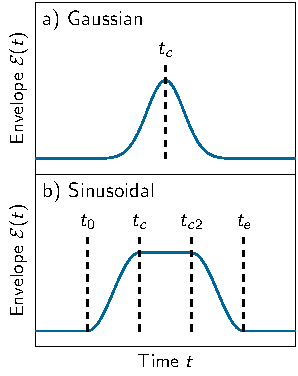
\includegraphics[scale=1]{img/laser_envelope/laser_envelope.pdf}
  \caption{Types of laser envelopes implemented in \ttt{laser.x}.}
  \label{fig:laser_envelope}
\end{figure}

\subsection{Field functions}

The field function $f(t)$ is defined as:
\begin{equation}
  f(t)=\E^{\I \left(\omega_0(t-t_c)+\phi\right)},
\end{equation}
where $\omega_0$ is the central frequency and $\phi$ is the phase of the pulse. Even though the laser field is complex in this expression, in the propagation of the electronic wavefunction in \sharc\ only the real part is used.

\subsection{Chirped pulses}

In order to apply a chirp to the laser pulse $l(t)$, it is first Fourier transformed to the frequency domain, giving the function $\tilde{l}(\omega)$. The chirp is applied by calculating:
\begin{equation}
  \tilde{l}^\prime(\omega)=
  \tilde{l}(\omega)
  \E^{-i\left[
  b_1|\omega-\omega_0|
  +\frac{b_2}{2}(\omega-\omega_0)^2
  +\frac{b_3}{6}(\omega-\omega_0)^3
  +\frac{b_4}{24}(\omega-\omega_0)^4
  \right]}\label{eq:laser_chirp}
\end{equation}
The chirped laser in the time domain $l^\prime(t)$ is then obtained by Fourier transform of the chirped pulse $\tilde{l}^\prime(\omega)$.


\subsection{Quadratic chirp without Fourier transform}

If the \ttt{fftw} package is not available, \ttt{laser.x} still can calculate analytical quadratic chirps for Gaussian pulses:
%%tth: \begin{equation} 
%%tth:   l(t)=\mathcal{E}_0^\prime\E^{-\I\left(\omega_0(t-t_c)+a_2(t-t_c)^2+\phi\right)}
%%tth: \end{equation}
%%tth: \begin{equation} 
%%tth:   \beta=\frac{4\ln 2}{\mathrm{FWHM}^2}
%%tth: \end{equation}
%%tth: \begin{equation} 
%%tth:   \beta^\prime=\frac{1}{\frac{1}{\beta}+4\beta b_2^2}
%%tth: \end{equation}
%%tth: \begin{equation} 
%%tth:   a_2=\frac{b_2}{\frac{1}{4\beta^2}+b^2_2}
%%tth: \end{equation}
%%tth: \begin{equation} 
%%tth:   \mathcal{E}_0^\prime=\mathcal{E}_0\sqrt{\frac{1}{2\I b_2\beta+1}}
%%tth: \end{equation}
\tthdump{
  \begin{align}
    l(t)=&
    \mathcal{E}_0^\prime
    \E^{-\beta^\prime(t-t_c)^2}
    \E^{-\I\left(
      \omega_0(t-t_c)+a_2(t-t_c)^2+\phi
    \right)}\\
    \beta=&\frac{4\ln 2}{\mathrm{FWHM}^2}\\
    \beta^\prime=&\frac{1}{\frac{1}{\beta}+4\beta b_2^2}\\
    a_2=&\frac{b_2}{\frac{1}{4\beta^2}+b^2_2}\\
    \mathcal{E}_0^\prime=&\mathcal{E}_0\sqrt{\frac{1}{2\I b_2\beta+1}}
  \end{align}
}
However, other chirps are only possible with the Fourier transformation.


\section{Laser interactions}\label{met:laser}

The laser field $\boldsymbol{\epsilon}$ is included in the propagation of the electronic wavefunction. In each substep of the propagation, the interaction of the laser field with the dipole moments is included in the Hamiltonian. The contribution $\vec{V}_i$ is in each timestep added to the Hamiltonian in equations~\eqref{eq:ham_propn} or \eqref{eq:ham_propl}, respectively:
%%tth: \begin{equation} 
%%tth:   \vec{V}_i=-\Re\left(\boldsymbol{\mu}_i\cdot\boldsymbol{\epsilon}_i\right),
%%tth: \end{equation}
%%tth: \begin{equation} 
%%tth:   \boldsymbol{\mu}_i=\boldsymbol{\mu}^{\text{MCH}}(t) + \frac{i}{n}\left(\boldsymbol{\mu}^{\text{MCH}}(t+\Delta t)-\boldsymbol{\mu}^{\text{MCH}}(t)\right),
%%tth: \end{equation}
%%tth: \begin{equation} 
%%tth:   \boldsymbol{\epsilon}_i=\boldsymbol{\epsilon}\left(t+\frac{i}{n}\Delta t\right)
%%tth: \end{equation}
\tthdump{
  \begin{align}
    \vec{V}_i=&
    -
    \Re\left(
      \boldsymbol{\mu}_i\cdot
      \boldsymbol{\epsilon}_i
    \right),\\
    \boldsymbol{\mu}_i=&
    \boldsymbol{\mu}^{\text{MCH}}(t) + \frac{i}{n}
    \left(
      \boldsymbol{\mu}^{\text{MCH}}(t+\Delta t)-\boldsymbol{\mu}^{\text{MCH}}(t)
    \right),\\
    \boldsymbol{\epsilon}_i=&\boldsymbol{\epsilon}\left(t+\frac{i}{n}\Delta t\right)
  \end{align}
}
where $i$, $n$ $t$ and $\Delta t$ are defined as in section \ref{met:propagate}.

\subsection{Surface Hopping with laser fields}

If laser fields are present, there can be two fundamentally different types of hops: laser-induced hops and non-adiabatic hops. The latter ones are the same hops as in the laser-free simulations, and demand that the total energy is conserved. The laser-induced hops on the other hand demand that the momentum (kinetic energy) is conserved. Hence, \sharc\ needs to decide for every hop whether it is laser-induced or not. 

Consider a previous state $\alpha$ and a new state $\beta$. Currently, the hop is classified based on the energy gap $\Delta E=|E_\beta^\text{diag}-E_\alpha^\text{diag}|$ and the instantaneous central energy of the laser pulse $\omega$. 
The hop is assumed to be laser-induced if
\begin{equation}
  |\Delta E-\omega| < W,
\end{equation}
where $W$ is a fixed parameter. $W$ can be set using the input keyword \ttt{laserwidth}.

If a hop has been classified as laser-free, the momentum is adjusted according to the equations given in section~\ref{met:ekinadj}.

\section{Phase tracking}

\subsection{Phase tracking of the transformation matrix}\label{met:phase_track}

A Hermitian matrix $\vec{H}^{\text{MCH}}$ can always be diagonalized. Its eigenvectors form the rows of a unitary matrix $\vec{U}$, which can be used to transform between the original basis and the basis of the eigenfunctions of $\vec{H}$. 
\begin{equation}
  \vec{H}^{\text{diag}}=\vec{U}^\dagger\vec{H}^{\text{MCH}}\vec{U}.
\end{equation}

However, the condition that $\vec{U}$ diagonalizes $\vec{H}^{\text{MCH}}$ is not sufficient to define $\vec{U}$ uniquely. Each normalized eigenvector $\vec{u}$ can be multiplied by a complex number on the unit circle and still remains a normalized eigenvector:
%%tth: \begin{equation} 
%%tth:   \vec{H}\vec{u}=h\vec{u}\qquad\text{and}\qquad\vec{u}^\dagger\vec{u}=1
%%tth: \end{equation}
%%tth: \begin{equation} 
%%tth:   \Rightarrow\nonumber
%%tth: \end{equation}
%%tth: \begin{equation} 
%%tth:   \vec{H}\left(\E^{\I\phi}\vec{u}\right)=\E^{\I\phi}\left(\vec{H}\vec{u}\right)=\E^{\I\phi}h\vec{u} =h\left(\E^{\I\phi}\vec{u}\right)
%%tth: \end{equation}
%%tth: \begin{equation} 
%%tth:   \text{and}
%%tth: \end{equation}
%%tth: \begin{equation} 
%%tth:   \left(\E^{\I\phi}\vec{u}\right)^\dagger\left(\E^{\I\phi}\vec{u}\right)=\vec{u}^\dagger\E^{-\I\phi}\E^{\I\phi}\vec{u}=\vec{u}^\dagger\vec{u}=1
%%tth: \end{equation}
\tthdump{
  \begin{align}
    \vec{H}\vec{u}=h\vec{u}
    \qquad&\text{and}\qquad
    \vec{u}^\dagger\vec{u}=1\\
    &\Rightarrow\nonumber\\
    \vec{H}\left(\E^{\I\phi}\vec{u}\right)
    =\E^{\I\phi}\left(\vec{H}\vec{u}\right)
    &=\E^{\I\phi}h\vec{u}
    =h\left(\E^{\I\phi}\vec{u}\right)\\
    &\text{and}\nonumber\\
    \left(\E^{\I\phi}\vec{u}\right)^\dagger\left(\E^{\I\phi}\vec{u}\right)
    =\vec{u}^\dagger\E^{-\I\phi}&\E^{\I\phi}\vec{u}
    =\vec{u}^\dagger\vec{u}=1
  \end{align}
}
Thus, for all diagonal matrices $\boldsymbol{\Phi}$ with elements $\delta_{\beta\alpha}\E^{\I\phi_\beta}$, also the matrix $\vec{U}^\prime=\vec{U}\boldsymbol{\Phi}$ diagonalizes $\vec{H}^{\text{MCH}}$ (if $\vec{U}$ diagonalizes it).

The propagation of the coefficients in the diagonal basis is written as (see section~\ref{met:propagate}):
\begin{equation}
  \vec{c}^{\text{diag}}(t+\Delta t)=\underbrace{\vec{U}^\dagger(t+\Delta t)\vec{R}^{\text{MCH}}(t+\Delta t,t)\vec{U}(t)}_{\vec{R}^{\text{diag}}(t+\Delta t,t)}\vec{c}^{\text{diag}}(t)
\end{equation}
where $\vec{U}(t)$ and $\vec{U}(t+\Delta t)$ are determined independently from diagonalizing the matrices $\vec{H}^{\text{MCH}}(t)$ and $\vec{H}^{\text{MCH}}(t+\Delta t)$, respectively. However, depending on the implementation of the diagonalization, $\vec{U}(t)$ and $\vec{U}(t+\Delta t)$ may carry unrelated, random phases. Even if $\vec{H}^{\text{MCH}}(t)$ and $\vec{H}^{\text{MCH}}(t+\Delta t)$ were identical, $\vec{U}(t)$ and $\vec{U}(t+\Delta t)$ might still differ, e.g.:
%%tth:\newline \includegraphics[scale=1]{equations/equation_51.gif}\newline
\tthdump{
  \begin{equation}
    \vec{U}(0)=
    \begin{pmatrix}1&0\\0&1\end{pmatrix}
    \qquad\text{and}\qquad 
    \vec{U}(t)=
    \begin{pmatrix}\I&0\\0&-\I\end{pmatrix}
  \end{equation}
}
The result is that the coefficients $\vec{c}$ pick up random phases during the propagation, leading to random changes in the direction of population transfer, invalidating the whole propagation.

In order to make the phases of $\vec{U}(t)$ and $\vec{U}(t+\Delta t)$ as similar as possible, \sharc\ employs a projection technique. First, we define the overlap matrix $\vec{V}$ between $\vec{U}(t)$ and $\vec{U}(t+\Delta t)$:
\begin{equation}
  \vec{V}=\vec{U}^\dagger(t+\Delta t)\vec{U}(t)
\end{equation}
For $\Delta t=0$, clearly
\begin{equation}
  \vec{U}(t+\Delta t)\vec{V}=\vec{U}(t)
\end{equation}
and $\vec{V}$ can be identified with the phase matrix $\boldsymbol{\Phi}$.

For $\Delta t\neq 0$, we must now find a matrix $\vec{P}$ so that
\begin{equation}
  \vec{U}(t+\Delta t)\vec{P}=\vec{U}^\prime(t+\Delta t)
\end{equation}
still diagonalizes $\vec{H}^{\text{MCH}}(t+\Delta t)$, but which minimizes the phase change with regard to $\vec{U}(t)$.
The matrix $\vec{P}$ has elements
\begin{equation}
  P_{\beta\alpha}=V_{\beta\alpha}
  \delta\left(
    E_\beta-E_\alpha
  \right).
\end{equation}
where $E_\beta$ is the $\beta$-th eigenvalue of $\vec{H}^{\text{MCH}}(t+\Delta t)$.

Within the \sharc\ algorithm, the phase of $\vec{U}(t+\Delta t)$ is adjusted to be most similar to $\vec{U}(t)$ by calculating first $\vec{V}$, generating $\vec{P}$ from $\vec{V}$ and the eigenvalues of $\vec{H}^{\text{MCH}}(t+\Delta t)$ and calculating the phase-corrected matrix $\vec{U}^\prime(t+\Delta t)$ as $\vec{U}(t+\Delta t)\vec{P}$.

\subsection{Tracking of the phase of the MCH wavefunctions}

Additionally, within the quantum chemistry programs, the phases of the electronic wavefunctions may change from one timestep to the next one. This will result in changes of the phase of all off-diagonal matrix elements (spin-orbit couplings, transition dipole moments, non-adiabatic couplings). \sharc\ has several possibilities to correct for that:
\begin{itemize}
  \item The interface can provide wavefunction phases through \ttt{QM.out}.
  \item If the overlap matrix is available, its diagonal contains the necessary phase information.
  \item Otherwise the scalar products of old and new non-adiabatic couplings and the relative phase of SOC matrix elements can be used to construct phase information.
\end{itemize}


\section{Random initial velocities}\label{met:veloc}

Random initial velocities are calculated with a given amount of kinetic energy $E$ per atom $a$. For each atom, the velocity is calculated as follows, with two uniform random numbers $\theta$ and $\phi$, from the interval $[0,1[$:
%%tth: \newline\includegraphics[scale=1]{equations/equation_47.gif}\newline
\tthdump{
  \begin{equation}
    \vec{v}=\sqrt{2E/m_a}
    \begin{pmatrix}
      \cos{\theta}\sin{\phi}\\
      \sin{\theta}\sin{\phi}\\
      \cos{\phi}
    \end{pmatrix}
  \end{equation}
}
This procedure gives a uniform probability distribution on a sphere with radius $\sqrt{2E/m_a}$.

Note that the translational and rotational components of random initial velocities are not projected out in the current implementation.

Random initial velocities can be requested in the input with \ttt{veloc random $E$}, where $E$ is a float defining the kinetic energy per atom (in eV).


\section{Representations}

Within \sharc, two different representations for the electronic states are used. The first is the so-called MCH basis, which is the basis of the eigenfunctions of the molecular Coulomb Hamiltonian. The molecular Coulomb Hamiltonian is the standard electronic Hamiltonian employed by the majority of quantum chemistry programs. It contains only the kinetic energy of the electrons and the potential energy arising from the Coulomb interaction between the electrons and nuclei.
\begin{equation}
  \hat{H}_{\text{el}}^{\text{MCH}}
  =\hat{K}_{\text{e}}
  +\hat{V}_{\text{ee}}
  +\hat{V}_{\text{ne}}
  +\hat{V}_{\text{nn}}.
\end{equation}
With this hamiltonian, states of the same multiplicity couple via the non-adiabatic couplings, while states of different multiplicity do not interact at all. 

The second representation used in \sharc\ is the so-called diagonal representation. It is the basis of the eigenfunctions of the total Hamiltonian.
\begin{equation}
  \hat{H}_{\text{el}}^{\text{total}}
  =\hat{H}_{\text{el}}^{\text{MCH}}
  +\hat{H}_{\text{el}}^{\text{coup}}.
\end{equation}
The term $\hat{H}_{\text{el}}^{\text{coup}}$ contains additional couplings not contained in the molecular Coulomb Hamiltonian. The most common couplings are spin-orbit couplings and interactions with an external electric field.
\begin{equation}
  \hat{H}_{\text{el}}^{\text{coup}}=\hat{H}_{\text{el}}^{\text{SOC}}-\boldsymbol{\mu}\boldsymbol{\epsilon}^{\text{ext}}
\end{equation}
Both of these couplings introduce off-diagonal elements in the total Hamiltonian. Thus, the eigenfunctions of the molecular Coulomb Hamiltonian are not the eigenfunctions of the total Hamiltonian. 

Within \sharc, usually quantum chemistry information is read in the MCH representation, while the surface hopping is performed in the diagonal one.

\subsection{Current state in MCH representation}\label{ssec:state_transform}

Oftentimes, it is very useful to know to which MCH state the currently active diagonal state corresponds. If $\hat{H}_{\text{el}}^{\text{coup}}$ is small or the state separation is large, then each diagonal state approximately corresponds to one MCH state. Only in the case of large couplings and/or near-degenerate states are the MCH states strongly mixed in the diagonal states.

In order to obtain for a given timestep from the currently active diagonal state $\beta$ the corresponding MCH state $\alpha$, a vector $\vec{c}^\text{diag}$ with $c_i^\text{diag}=\delta_{i\beta}$ is generated. The vector is transformed into the MCH representation
\begin{equation}
  \vec{c}^\text{MCH}=\vec{U}\vec{c}^\text{diag}.
\end{equation}
The corresponding MCH state $\alpha$ is the index of the (absolute) largest element of vector $\vec{c}^\text{MCH}$.


\section{Sampling from Wigner Distribution}\label{met:wigner}

The sampling is based on references~\cite{Dahl1988JCP, Schinke1995}.

The frequency calculation provides a set of vibrational frequencies $\{\nu_i\}$ and the corresponding normal mode vectors $\{\vec{n}_i\}$, where $i$ runs from 1 to $N=3*n_{\text{atom}}$. It also provides the equilibrium geometry $\vec{R}_{\text{eq}}$.

In order to create an initial condition $(\vec{R},\vec{v})$, the following procedure is applied. Initially, $\vec{R}_0=\vec{R}_{\text{eq}}$ and $\vec{v}_0)=0$. Then, for each normal mode $i$, two random numbers $P_i$ and $Q_i$ are chosen uniformly from the interval $[-3,3]$. The value of a ground state quantum Wigner distribution for these values is calculated:
\begin{equation}
  W_i=\E^{-P_i^2}\E^{-Q_i^2}.
\end{equation}
$W_i$ is compared to a uniform random $r_i$ number from $[0,1]$. If $W_i>r_i$, then $P_i$ and $Q_i$ are accepted and the coordinates and velocities are updated:
%%tth: \begin{equation}
%%tth:   \vec{R}_i=\vec{R}_{i-1} + \frac{Q}{\sqrt{2\nu_i}}\vec{n}_i
%%tth: \end{equation}
%%tth: \begin{equation}
%%tth:   \vec{v}_i=\vec{v}_{i-1} + \frac{P\sqrt{\nu_i}}{\sqrt{2}}\vec{n}_i
%%tth: \end{equation}
\tthdump{
  \begin{align}
    \vec{R}_i=&\vec{R}_{i-1} + \frac{Q}{\sqrt{2\nu_i}}\vec{n}_i\\
    \vec{v}_i=&\vec{v}_{i-1} + \frac{P\sqrt{\nu_i}}{\sqrt{2}}\vec{n}_i\\
  \end{align}
}
The random number procedure and updates are repeated for all normal modes, until $(\vec{R}_N,\vec{v})_N$ is obtained, which constitutes one initial condition. Finally, the center of mass is restored and translational and rotational components are projected out of $\vec{v}$. The harmonic potential energy is given by:
\begin{equation}
  E_{\text{pot}}=\frac{1}{2}\sum\limits_i \nu_iQ_i^2
\end{equation}


\section{Scaling}

The scaling factor (keyword \ttt{scaling}) applies to all energies and derivatives of energies. Hence, the full Hamiltonian is scaled, and the gradients are scaled. Nothing else is scaled (no dipole moments, non-adiabatic couplings, overlaps, etc).


\section{Seeding of the RNG}

The standard Fortran 90 random number generator is seeded by a sequence of integers of length $n$, where $n$ depends on the computer architecture. The input of \sharc, however, takes only a single RNG seed, which must reproducibly produce the same sequence of random numbers for the same input.

In order to generate the seed sequence from the single input $x$, the following procedure is applied:
\begin{itemize}
  \item Query for the number $n$,
  \item Generate a first seed sequence $\vec{s}$ with $s_i=x+37i+17i^2$,
  \item Seed with the sequence $\vec{s}$,
  \item Obtain a sequence $\vec{r}$ of $n$ random numbers on the interval $[0,1[$,
  \item Generate a second seed sequence $\vec{s}^\prime$ with $s_i^\prime=\text{int}\left(65536(r_i-\frac{1}{2})\right)$,
  \item Reseed with the sequence $\vec{s}^\prime$.
\end{itemize}
The fifth step will generate a sequence of nearly uncorrelated numbers, distributed uniformly over the full range of possible integer values. 


\section{Selection of gradients and non-adiabatic couplings}\label{met:selection}

In order to increase performance, it is possible to omit the calculation of certain gradients and non-adiabatic couplings. An energy-gap-based algorithm selects at each timestep a subset of all possible gradients and non-adiabatic couplings to be calculated. Given the diagonal energy $E^{\text{diag}}_\xi$ of the current active state $\xi$, the gradient $\vec{g}^{\text{MCH}}_\alpha$ of MCH state $\alpha$ is calculated if:
\begin{equation}
  \left|
    E^{\text{diag}}_\xi - E^{\text{MCH}}_\alpha
  \right|
  <
  \varepsilon_\text{grad}
\end{equation}
where $\varepsilon_\text{grad}$ is the selection threshold.

Similarly, a non-adiabatic coupling vector $\vec{K}^{\text{MCH}}_{\beta\alpha}$ is calculated if:
\begin{equation}
  \left|
    E^{\text{diag}}_\xi - E^{\text{MCH}}_\alpha
  \right|
  <
  \varepsilon_\text{nac}
  \qquad\text{and}\qquad
  \left|
    E^{\text{diag}}_\xi - E^{\text{MCH}}_\beta
  \right|
  <
  \varepsilon_\text{nac}
\end{equation}
with selection threshold $\varepsilon_\text{nac}$.

Neither $\vec{g}^{\text{MCH}}_\alpha$ nor $\vec{K}^{\text{MCH}}_{\beta\alpha}$ are ever calculated if $\alpha$ or $\beta$ are frozen states.

There is only one keyword (\ttt{eselect}) to set the selection threshold, so $\varepsilon_\text{grad}$ and $\varepsilon_\text{nac}$ are the same in most cases. 


\section{State ordering}\label{met:ordering}

The canonical ordering of MCH states of different $S$ and $M_S$ in \sharc\ is as follows. In the innermost loop, the quantum number is increased; then $M_S$ and finally $S$. Example:

% \begin{example}
  \verb|nstates 3 0 3|

  Order of states:

  \begin{tabular}{rlccc}
    \toprule
    Number      &Label       &$S$ &$M_S$  &$n$\\
    \midrule
    1&$S_0$       &0&0&1\\
    2&$S_1$       &0&0&2\\
    3&$S_2$       &0&0&3\\
    4&$T_1^-$       &2&-1&1\\
    5&$T_2^-$       &2&-1&2\\
    6&$T_3^-$       &2&-1&3\\
    7&$T_1^0$       &2&0&1\\
    8&$T_2^0$       &2&0&2\\
    9&$T_3^0$       &2&0&3\\
    10&$T_1^+$       &2&+1&1\\
    11&$T_2^+$       &2&+1&2\\
    12&$T_3^+$       &2&+1&3\\
    \bottomrule
  \end{tabular}
% \end{example}

The canonical ordering of states is for example important in order to specify the initial state in the MCH basis (using the \ttt{state} keyword in the input file).


\section{Surface Hopping}

Given two coefficient vectors $\vec{c}^{\text{diag}}(t)$ and $\vec{c}^{\text{diag}}(t+\Delta t)$ and the corresponding propagator matrix $\vec{R}^{\text{MCH}}(t+\Delta t,t)$, the surface hopping probabilities are given by
\begin{equation}
  P_{\beta\rightarrow\alpha}=
  \left(
    1-
    \frac{
      \left|
        c_\beta^{\text{diag}}(t+\Delta t)
      \right|^2
    }{
      \left|
        c_\beta^{\text{diag}}(t)
      \right|^2
    }\right)
    \times
    \frac{
      \Re\left[
        c^{\text{diag}}_\alpha(t+\Delta t)
        R^*_{\alpha\beta}
        \left(
          c^{\text{diag}}_\beta(t)
        \right)^*
      \right]
    }{
      \left|
        c^{\text{diag}}_\beta(t)
      \right|^2
      -\Re\left[
        c^{\text{diag}}_\beta(t+\Delta t)
        R^*_{\beta\beta}
        \left(
          c^{\text{diag}}_\beta(t)
        \right)^*
      \right]
    }.
\end{equation}
where, however, $P_{\beta\rightarrow\beta}=0$ and all negative $P_{\beta\rightarrow\alpha}$ are set to zero.

The hopping procedure itself obtains a uniform random number $r$ from the interval $[0,1]$. A hop to state $\alpha$ is performed, if
\begin{equation}
  \sum\limits_{i=1}^{\alpha-1} P_{\beta\rightarrow i} < r \le P_{\beta\rightarrow\alpha}+\sum\limits_{i=1}^{\alpha-1} P_{\beta\rightarrow i}
\end{equation}
See section~\ref{met:ekinadj} for further details on how frustrated hops are handled.


\section{Velocity Verlet}

The nuclear coordinates of atom $A$ are updated according to the Velocity Verlet algorithm \cite{Verlet1967PR}, based on the gradient of state $\beta$ at $\vec{R}(t)$ and $\vec{R}(t+\Delta t)$:
%%tth: \begin{equation}
%%tth:   \vec{a}_A(t)=-\frac{1}{m_A}\nabla_{\vec{R_A}}E_\beta(\vec{R}(t))
%%tth: \end{equation}
%%tth: \begin{equation}
%%tth:   \vec{a}_A(t+\Delta t)=-\frac{1}{m_A}\nabla_{\vec{R_A}}E_\beta(\vec{R}(t+\Delta t))
%%tth: \end{equation}
%%tth: \begin{equation}
%%tth:   \vec{R}_A(t+\Delta t)=\vec{R}_A(t)+\vec{v}_A(t)\Delta t + \frac{1}{2}\vec{a}_A(t)\Delta t^2
%%tth: \end{equation}
%%tth: \begin{equation}
%%tth:   \vec{v}_A(t+\Delta t)=\vec{v}_A(t)+\frac{1}{2}\left[\vec{a}_A(t)+\vec{a}_A(t+\Delta t)\right]\Delta t
%%tth: \end{equation}
\tthdump{
  \begin{align}
    \vec{a}_A(t)=&
    -\frac{1}{m_A}\nabla_{\vec{R_A}}E_\beta(\vec{R}(t))\\
    \vec{a}_A(t+\Delta t)=&
    -\frac{1}{m_A}\nabla_{\vec{R_A}}E_\beta(\vec{R}(t+\Delta t))\\
    \vec{R}_A(t+\Delta t)=&
    \vec{R}_A(t)+\vec{v}_A(t)\Delta t + \frac{1}{2}\vec{a}_A(t)\Delta t^2\\
    \vec{v}_A(t+\Delta t)=&
    \vec{v}_A(t)+\frac{1}{2}\left[\vec{a}_A(t)+\vec{a}_A(t+\Delta t)\right]\Delta t
  \end{align}
}

Currently, there are no other integrators for the nuclear motion implemented in \sharc.


\section{Wavefunction propagation}\label{met:propagate}

The electronic wavefunction is needed in order to carry out surface hopping. The electronic wavefunction is expanded in the basis of the so-called model space $\mathcal{S}$, which includes the few lowest states $|\psi^{\text{MCH}}_\alpha\rangle$ of the multiplicities under consideration (e.g.\ the 3 lowest singlet and 2 lowest triplet states). 
\begin{equation}
  \Psi_{\text{el}}(t)=\sum\limits_{\alpha\in\mathcal{S}} c^{\text{MCH}}_\alpha \left|\psi^{\text{MCH}}_\alpha\right\rangle
\end{equation}
All multiplet components are included explicitly, i.e., the inclusion of an MCH triplet state adds three explicit states to the model space (the three components of the triplet).

Within \sharc, the wavefunction is represented just by the vector $\vec{c}^{\text{MCH}}$. The Hamiltonian $\vec{H}^{\text{MCH}}$ is represented in matrix form with elements:
\begin{equation}
  H^{\text{MCH}}_{\beta\alpha}=\left\langle\psi^{\text{MCH}}_\beta\middle|\hat{H}_{\text{el}}^{\text{total}}\middle|\psi^{\text{MCH}}_\alpha\right\rangle
\end{equation}

From the MCH representation, the diagonal representation can be obtained by unitary transformation within the model space $\mathcal{S}$ ($\vec{U}^\dagger\vec{H}^{\text{MCH}}\vec{U}=\vec{H}^{\text{diag}}$ and $\vec{U}^\dagger\vec{c}^{\text{MCH}}=\vec{c}^{\text{diag}}$):
\begin{equation}
  \Psi_{\text{el}}(t)=\sum\limits_{\alpha\in\mathcal{S}} c^{\text{diag}}_\alpha \left|\psi^{\text{diag}}_\alpha\right\rangle
\end{equation}
and
\begin{equation}
  H^{\text{diag}}_{\beta\alpha}=\left\langle\psi^{\text{diag}}_\beta\middle|\hat{H}_{\text{el}}^{\text{total}}\middle|\psi^{\text{diag}}_\alpha\right\rangle
\end{equation}

The propagation of the electronic wavefunction from time $t$ to $t+\Delta t$ can then be written as the product of a propagation matrix with the coefficients at time $t$:
\begin{equation}
  \vec{c}^{\text{diag}}(t+\Delta t)=\vec{R}^{\text{diag}}(t+\Delta t,t)\vec{c}^{\text{diag}}(t)
\end{equation}
or
\begin{equation}
  \vec{c}^{\text{diag}}(t+\Delta t)=\underbrace{\vec{U}^\dagger(t+\Delta t)\vec{R}^{\text{MCH}}(t+\Delta t,t)\vec{U}(t)}_{\vec{R}^{\text{diag}}(t+\Delta t,t)}\vec{c}^{\text{diag}}(t)
\end{equation}

In order to calculate $\vec{R}^{\text{MCH}}(t+\Delta t,t)$, \sharc\ uses (unitary) operator exponentials. 

\subsection{Propagation using non-adiabatic couplings}

Here we assume that in the dynamics the interaction between the electronic states is described by a matrix of non-adiabatic couplings $\vec{K}^{\text{MCH}}(t)$, such that
\begin{equation}
  \left(\vec{K}^{\text{MCH}}(t)\right)_{\beta\alpha}
  =
  \left\langle
    \psi_\beta(t)
  \middle|
    \frac{\partial}{\partial t}
  \middle|
    \psi_\alpha(t)
  \right\rangle
  \label{eq:ddt}
\end{equation}
or
\begin{equation}
  \left(\vec{K}^{\text{MCH}}(t)\right)_{\beta\alpha}
  =
  \frac{\partial \vec{R}}{\partial t}\cdot
  \left\langle
    \psi_\beta(t)
  \middle|
    \frac{\partial}{\partial \vec{R}}
  \middle|
    \psi_\alpha(t)
  \right\rangle.
  \label{eq:ddr}
\end{equation}
In equation~\eqref{eq:ddt}, the time-derivative couplings are directly calculated by the quantum chemistry program (use \ttt{coupling ddt} in the \sharc\ input), while in~\eqref{eq:ddr} the matrix $\vec{K}^{\text{MCH}}(t)$ is obtained from the scalar product of the nuclear velocity and the non-adiabatic coupling vectors (use \ttt{coupling ddr} in the input).

The propagation matrix can then be written as 
\begin{equation}
  \vec{R}^{\text{MCH}}(t+\Delta t,t)=
  \hat{\mathfrak{T}}
  \exp\left[
    -\int\limits_{t}^{t+\Delta t}
    \left(
      \frac{\I}{\hbar}\vec{H}^{\text{MCH}}(\tau)+\vec{K}^{\text{MCH}}(\tau) 
    \right)\D\tau
  \right]
\end{equation}
with the time-ordering operator $\hat{\mathfrak{T}}$. For small timesteps $\Delta t$, $\vec{H}^{\text{MCH}}(\tau)$ and $\vec{K}^{\text{MCH}}(\tau)$ can be interpolated linearly
\begin{equation}
  \vec{R}^{\text{MCH}}(t+\Delta t,t)=
  \exp\left[
    -\frac{1}{2}\left(
      \frac{\I}{\hbar}\vec{H}^{\text{MCH}}(t)+\frac{\I}{\hbar}\vec{H}^{\text{MCH}}(t+\Delta t)
      +\vec{K}^{\text{MCH}}(t)+\vec{K}^{\text{MCH}}(t+\Delta t)
    \right)\Delta t
  \right]
\end{equation}
And in order to have a sufficiently small timestep for this to work, the interval $(t,t+\Delta t)$ is further split into subtimesteps $\Delta\tau=\frac{\Delta t}{n}$. 
%%tth: \begin{equation}
%%tth:   \vec{R}^{\text{MCH}}(t+\Delta t,t)=\prod\limits_{i=1}^{n}\vec{R}_i
%%tth: \end{equation}
%%tth: \begin{equation}
%%tth:   \vec{R}_i=\exp\left[-\left(\frac{\I}{\hbar}\vec{H}_i+\vec{K}_i\right)\Delta\tau\right]
%%tth: \end{equation}
%%tth: \begin{equation}
%%tth:   \vec{H}_i=\vec{H}^{\text{MCH}}(t) + \frac{i}{n}\left(\vec{H}^{\text{MCH}}(t+\Delta t)-\vec{H}^{\text{MCH}}(t)\right)\label{eq:ham_propn}
%%tth: \end{equation}
%%tth: \begin{equation}
%%tth:   \vec{K}_i=\vec{K}^{\text{MCH}}(t) + \frac{i}{n}\left(\vec{K}^{\text{MCH}}(t+\Delta t)-\vec{K}^{\text{MCH}}(t)\right)
%%tth: \end{equation}
\tthdump{
  \begin{align}
    \vec{R}^{\text{MCH}}(t+\Delta t,t)=&
    \prod\limits_{i=1}^{n}
    \vec{R}_i\\
    \vec{R}_i=&
    \exp\left[
        -\left(
          \frac{\I}{\hbar}\vec{H}_i
          +\vec{K}_i
        \right)\Delta\tau
    \right]\\
    \vec{H}_i=&
    \vec{H}^{\text{MCH}}(t) + \frac{i}{n}
    \left(
      \vec{H}^{\text{MCH}}(t+\Delta t)-\vec{H}^{\text{MCH}}(t)
    \right)\label{eq:ham_propn}\\
    \vec{K}_i=&
    \vec{K}^{\text{MCH}}(t) + \frac{i}{n}
    \left(
      \vec{K}^{\text{MCH}}(t+\Delta t)-\vec{K}^{\text{MCH}}(t)
    \right)
  \end{align}
}

\subsection{Propagation using overlap matrices}

In many situations, the non-adiabatic couplings in $\vec{K}^{\text{MCH}}$ are very localized on the potential hypersurfaces. If this is the case, in the dynamics very short timesteps are necessary to properly sample the non-adiabatic couplings. If too large timesteps are used, part of the coupling may be missed, leading to wrong population transfer. The local diabatization algorithm gives more numerical stability in these situations. It can be requested with the line \ttt{coupling overlap} in the input file.

Within this algorithm, the change of the electronic states between timesteps is described by the overlap matrix $\vec{S}^{\text{MCH}}(t,t+\Delta t)$
\begin{equation}
  \left(\vec{S}^{\text{MCH}}(t,t+\Delta t)\right)_{\beta\alpha}=
  \left\langle
    \psi_\beta(t)
  \middle|
    \psi_\alpha(t+\Delta t)
  \right\rangle
\end{equation}

With this, the propagator matrix can be written as
%%tth: \begin{equation}
%%tth:   \vec{R}^{\text{MCH}}(t+\Delta t,t)=\vec{S}^{\text{MCH}}(t,t+\Delta t)^\dagger\prod\limits_{i=1}^{n}\vec{R}_i
%%tth: \end{equation}
%%tth: \begin{equation}
%%tth:   \vec{R}_i=\exp\left[-\frac{\I}{\hbar}\vec{H}_i\Delta\tau\right]
%%tth: \end{equation}
%%tth: \begin{equation}
%%tth:   \vec{H}_i=\vec{H}^{\text{MCH}}(t) + \frac{i}{n}\left(\vec{H}^{\text{MCH}}_{\text{tra}}-\vec{H}^{\text{MCH}}(t)\right)\label{eq:ham_propl}
%%tth: \end{equation}
%%tth: \begin{equation}
%%tth:   \vec{H}^{\text{MCH}}_{\text{tra}}=\vec{S}^{\text{MCH}}(t,t+\Delta t)\vec{H}^{\text{MCH}}(t+\Delta t)\vec{S}^{\text{MCH}}(t,t+\Delta t)^\dagger
%%tth: \end{equation}
\tthdump{
  \begin{align}
    \vec{R}^{\text{MCH}}(t+\Delta t,t)=&
    \vec{S}^{\text{MCH}}(t,t+\Delta t)^\dagger\prod\limits_{i=1}^{n}
    \vec{R}_i\\
    \vec{R}_i=&
    \exp\left[
        -\frac{\I}{\hbar}\vec{H}_i\Delta\tau
    \right]\\
    \vec{H}_i=&
    \vec{H}^{\text{MCH}}(t) + \frac{i}{n}
    \left(
      \vec{H}^{\text{MCH}}_{\text{tra}}
      -\vec{H}^{\text{MCH}}(t)
    \right)\label{eq:ham_propl}\\
    \vec{H}^{\text{MCH}}_{\text{tra}}=&
      \vec{S}^{\text{MCH}}(t,t+\Delta t)
      \vec{H}^{\text{MCH}}(t+\Delta t)
      \vec{S}^{\text{MCH}}(t,t+\Delta t)^\dagger
  \end{align}
}











%%tth: \chapter{Bibliography}
\begin{unnumbered}
  \tthdump{
    \phantomsection
    \addcontentsline{toc}{chapter}{Bibliography}
  }
  \bibliography{mai_bibliography}
  \bibliographystyle{paper-sebastian}
\end{unnumbered}

\end{document}
